\chapter{Model Independent Trilepton Search}\label{ch:model-independent-trilepton-search}

Events containing three or more leptons are useful probes of phenomena beyond the Standard Model. On one hand, the expected Standard Model backgrounds are typically small; depending on the kinematic requirements on the three leptons, such events arise dominantly from diboson production ($WZ$, $ZZ$), or from event where one or more leptons arises from misidentified or semileptonically decaying jets. On the other hand, the production of three or more leptons is predicted by many models of phenomena beyond the Standard Model, as described in section~\ref{sec:beyond-the-standard-model}. This dissertation presents two such searches: a model-independent search for non-resonant production of three or more leptons in many signal regions, and a signature-driven search for resonance trilepton production in the context of heavy leptons. 

This chapter presents a search for physics beyond the Standard Model using events containing three or more leptons. The search uses $20.3~\ifb$ of $pp$ collision data taken at $\sqrt{s}=8~\mbox{TeV}$ with the ATLAS detector. Many signal regions are defined based on the properties of the leptons, jets, and overall momentum imbalance of the event, with the goal of being broadly sensitive to the non-resonant production of trilepton final states by phenomena beyond the Standard Model. 

\section{Event Selection}\label{sec:model-independent-event-selection}

This section describes the selection of events containing at least three leptons in both $pp$ collision data and in the Monte Carlo simulation samples. 


\subsection{Object Definitions}\label{sec:model-independent-object-definitions}

\subsubsection{Leptons}\label{sec:model-independent-lepton-definitions}

The analysis requires at least three reconstructed electrons, muons, or hadronically decaying tau leptons, as described in section~\ref{sec:object-reconstruction}. A summary of the lepton selections is shown in table~\ref{table:lepton-selections}. Leptons are required to satisfy the following requirements:

\begin{itemize}

	\item \underline{\textbf{Transverse momentum}}: Electrons and muons must have $\pt>15 \GeV$, while hadronically decaying tau leptons must have $\pt>20 \GeV$. The transverse momentum cut is driven by the availability of triggers with which to perform the data-driven reducible background estimate, described in section~\label{sec:fake-factors}. 

	\item \underline{\textbf{Geometrical acceptance}}: Electrons are required to have $|\eta|<2.47$, excluding the transition region $1.37<|\eta|<1.52$ between the barrel and end-cap calorimeters. Muons and tau leptons are required to have $|\eta|<2.5$.

	\item \underline{\textbf{Particle identification}}: To suppress the reducible backgrounds, the leptons must satisfy strict requirements related to particle identification, as described in section~\ref{sec:object-reconstruction}. Electrons candidates must satisfy the tight++ set of identification cuts. Electrons are neglected if they fall in a region affected by the presence of a dead front end board in the first or second sampling layer, a dead high voltage supply, or a masked cell in the core. Muons are required to be \emph{combined}, with associated hits in the inner detector and muon spectrometer. Specifically, 
	\begin{itemize}
	  \item A B-layer hit (if expected).
	  \item $\geq1$ pixel hit and $\geq5$ SCT hits, including any dead sensors along the trajectory.
	  \item $<3$ total holes in the pixel and SCT. 
	  \item \textcolor{red}{Needs more explanation} If $0.1 < |\eta| < 1.9$, require $n_{\mathrm{TRT}}^{\mathrm{hits}}+n_{\mathrm{TRT}}^{\mathrm{outliers}} > 5$ and $n_{\mathrm{TRT}}^{\mathrm{outliers}} < 0.9 \times (n_{\mathrm{TRT}}^{\mathrm{hits}}+n_{\mathrm{TRT}}^{\mathrm{outliers}})$,
	 % \item Else if $|\eta| < 0.1$ or $|\eta| > 1.9$ and $n_{\mathrm{TRT}}^{\mathrm{hits}}+n_{\mathrm{TRT}}^{\mathrm{outliers}} > 5$, then require $n_{\mathrm{TRT}}^{\mathrm{outliers}} < 0.9 \times (n_{\mathrm{TRT}}^{\mathrm{hits}}+n_{\mathrm{TRT}}^{\mathrm{outliers}})$.
	\end{itemize}

	Finally, tau leptons must satisfy the \texttt{ BDT-tight} selection criteria.

	\item \underline{\textbf{Impact parameter}}: The inner detector track associated with electrons and muons must be consistent with originating from the event primary vertex. The transverse impact parameter significance, defined as the transverse impact parameter $d_0$ divided by its uncertainty $\sigma_{d_0}$, is required to satisfy $\frac{d_0}{\sigma_{d_0}}<3$. Similarly, the longitudinal impact parameter $z_0$ is required to satisfy $z_0\sin\theta < 0.5~\mm$. These requirements suppress leptons from semileptonic heavy flavor decays. 

	\item \underline{\textbf{Isolation}}: To further reduce the impact of non-prompt and misidentified leptons, the leptons are required to be isolated from other activity in the event. The cuts on electrons and muons are similar, and limit the amount of nearby activity as measured by inner detector tracks and calorimeter energy deposits:

	\begin{itemize}
		\item For both electrons and muons, a cut is applied on \verb.ptcone30., the sum of transverse momenta of tracks associated to the same primary vertex as the lepton within a cone of $\Delta R<0.3$. 
		\item For muons, a cut is applied on \verb.Etcone30., the scalar sum of transverse energies of calorimeter cells within $\Delta R<3.0$ of the muon track. 
		\item For electrons, a cut is applied on \verb.TopoEtcone30., the sum of topological calorimeter clusters within a cone of $\Delta R < 3.0$. The use of topological clusters reduces the impact of pileup and out-of-cone leakage. 
	\end{itemize}

	All isolation variables are required to be less than $10\%$ of the lepton transverse momentum for leptons with $\pt<100~\mbox{GeV}$, and less than $10~\mbox{GeV}+0.01\times \pt$ for leptons with $\pt\geq 100~\mbox{GeV}$. 
\end{itemize}

\begin{table}[h]
	\footnotesize
		\begin{tabular}{ccc}
			Cut & Electrons & Muons \\
			\hline
			Object ID & Tight++ & Combined Tight \\
			Leading (trigger) $\ET/\pt$ & $\ET>26~\mbox{GeV}$ & $\pt>26~\mbox{GeV}$ \\
			Subleading $\ET/\pt$ & $\ET>15~\mbox{GeV}$ & $\pt>15~\mbox{GeV}$ \\
			Trigger Acceptance & $(|\eta|<2.47)\ \&\&\ !(1.37<|\eta|<1.52)$ & $|\eta|<2.4$ \\
			Acceptance & $(|\eta|<2.47)\ \&\&\ !(1.37<|\eta|<1.52)$ & $|\eta|<2.5$ \\
			Calo. Isolation & \verb.TopoEtcone30. $<\left\{\begin{array}{ccl} 0.1\times \ET & : & \ET < 100~\mbox{GeV} \\ 10~\mbox{GeV}+0.01\times \ET & : & \ET>100~\mbox{GeV} \end{array}\right.$ & \verb.Etcone30. $<\left\{\begin{array}{ccl} 0.1\times \pt & : & \pt < 100~\mbox{GeV} \\ 10~\mbox{GeV}+0.01\times \pt & : & \pt>100~\mbox{GeV} \end{array}\right.$ \\
			Track Isolation & \verb.ptcone30. $<\left\{\begin{array}{ccl} 0.1\times \ET & : & \ET < 100~\mbox{GeV} \\ 10~\mbox{GeV}+0.01\times \ET & : & \ET>100~\mbox{GeV} \end{array}\right.$ & \verb.ptcone30. $<\left\{\begin{array}{ccl} 0.1\times \pt & : & \pt < 100~\mbox{GeV} \\ 10~\mbox{GeV}+0.01\times \pt & : & \pt>100~\mbox{GeV} \end{array}\right.$ \\
			Track $d_0$ & $\frac{d_0}{\sigma_{d_0}}<3$  \\
			Track $z_0$ & $z_0\sin\theta<0.5~\mbox{mm}$  \\
		\end{tabular}
	\caption{Detailed list of lepton selections.}
	\label{table:lepton-selections}
\end{table}

\subsubsection{Jets and Missing Transverse Energy}\label{sec:model-independent-jets-met}

Jets are reconstructed from topological clusters using the \antikt\ jet algorithm~\cite{Cacciari:2008gp} with a distance parameter of $R = 0.4$ and full four-momentum recombination and are calibrated with a local cluster weighting (LCW) algorithm ({AntiKt4LCTopoJets})~\cite{ATLAS-CONF-2010-053}. The LCW algorithm determines if a topological cluster in the calorimeter is of hadronic or electromagnetic origin, and applies the appropriate energy correction. The jet response also depends on pileup conditions; this is accounted for using the jet area subtraction method provided by the JetEtMiss group~\cite{JetEtmissRecommendations2012}.

Jets are required to have $\pt>30~\mbox{GeV}$, in order to limit the presence of pileup jets. For the geometrical acceptance, jets must lie in the range $|\eta|<4.5$, so that the jet falls within instrumented regions of the detector. Pileup jets are additionally suppressed with a cut on the jet vertex fraction: the $\sum \pt$ of tracks within the jet cone and associated with the selected primary vertex must be at least $50\%$ of the $\sum \pt$ of all tracks within the jet cone~\cite{jvf}. 

Jets consistent with originating from the decay of a $b$-hadron are identified using the MV1 algorithm~\cite{MV1}, with an efficiency of $80\%$. 

The missing transverse momentum, $\Etmiss$, is calculated using the \texttt{ MET\_Egamma10NoTau\_RefFinal} algorithm. Calorimeter cells associated with electrons or photons with $\pt>10 \GeV$ are calibrated specifically to that object; cells associated with tau leptons are not calibrated as tau leptons due to the change in the energy calibration for the objects used in the data-driven reducible background estimate~\ref{sec:fake-factors}. 

\subsection{Triggering}
Collisions events for this analysis are triggered using the unprescaled single-electron or single-muon triggers with the lowest transverse momentum thresholds. At least one of the following triggers must have fired:

\begin{itemize}
	\item \texttt{ EF\_e24vhi\_medium1}: One electron with $\pt>24 \GeV$. The electron must satisfy cuts similar to the medium++ identification criteria at the trigger level, an isolation requirement of $\frac{\pt^{\mathrm{cone}20}}{\pt}<0.1$, and cuts on the leakage into the hadronic calorimeter.
	\item \texttt{ EF\_e60\_medium1}: One electron with $\pt>60 \GeV$. The electron must also satisfy the medium identification cuts, but the isolation and leakage requirements are removed.
	\item \texttt{ EF\_mu24i\_tight}: One muon with $\pt>24 \GeV$, satisfying an isolation requirement of $\frac{\pt^{\mathrm{cone}20}}{\pt}<0.12$.
	\item \texttt{ EF\_mu36\_tight}: One muon with $\pt>36 \GeV$, with the isolation requirement removed.
\end{itemize}

The higher-threshold triggers without isolation requirements recover efficiency at higher $\pt$. Triggered events are required to have an offline lepton matched to the trigger object within $\Delta R=\sqrt{(\Delta\eta)^2+(\Delta\phi)^2} < 0.1$. To avoid trigger turn-on effects near the $\pt$ threshold, the offline lepton must have $\pt>26 \GeV$. Additionally, trigger-matched muon must have $|\eta|<2.4$ to avoid uninstrumented regions of the detector.

%Monte Carlo events are selected using the trigger simulation. The discrepancies between the trigger performance in data and Monte Carlo are usually smaller than 2\%~\cite{Ancu:1501709}. 

\subsection{Overlap Removal}\label{sec:model-independent-overlap-removal}
Objects are frequently reconstructed as multiple objects; for example, a muon with a hard bremsstrahlung emission might be reconstructed as a muon, an electron, and a jet. In order to resolve ambiguities, the following overlap removal procedure is applied:

\begin{itemize}
	\item If $\Delta R(e, e) < 0.1$, remove lower $\pt$ electron, to avoid ``a potential bias in the simulation of the reconstruction efficiency for two real, close-by same-flavour leptons''~\cite{Adams:1700874}.
	\item If $\Delta R(e, $jet$) < 0.2$, remove jet. This addresses the ambiguity between electrons and jets.
	\item If $0.2 < \Delta R($jet$, e) < 0.4$ AND $\pt($jet$) > 30~\mbox{GeV} + 0.05 * \pt(e)$, remove electron. This reduces the reducible electron backgrounds.
	\item If $\Delta R(\mu, e) < 0.1$, remove electron. This addresses cases where a muon radiates a hard photon, which is then identified as an electron.
	\item If $\Delta R(\mu, \mbox{jet})<0.1$, and:
	\begin{equation}
		\begin{array}{ccc}
			\pt^{\mathrm{jet}}<0.5 \pt^{\mu} & : & \pt^{\mu} < 200~\mbox{GeV},\ \mbox{or} \\
			\pt^{\mathrm{jet}}<100~\mbox{GeV} & : & \pt^{\mu} \geq 200~\mbox{GeV},
		\end{array}
	\end{equation}
	remove the jet. This is intended to reduce efficiency loss (in the next bullet point) from jets induced by muons at high muon $\pt$. 
	\item If $\Delta R($jet$, \mu) < 0.3$, remove muon. This reduces the reducible muon backgrounds.
\end{itemize}

% David edit: do we use MET anywhere in the analysis?
%\subsection{Missing Transverse Energy Definition} 
%\label{sec:Selection_MET}
%
%The \met\ is calculated from an object-based algorithm \texttt{ MET\_Egamma10NoTau\_RefFinal}~\cite{Aad:2012re}:
%
%\begin{equation}
%{\met}^{\mathrm{RefFinal}} = {\met}^{\mathrm{RefEle}} + {\met}^{\mathrm{RefJet}} + {\met}^{\mathrm{RefMuon}} + {\met}^{\mathrm{CellOut}} + {\met}^{\mathrm{RefGamma}}.
%\label{eqn:met}
%\end{equation}
%
%Muons passing the selection criteria and with $\pT > 10 \gev$ are included in the $ {\met}^{\mathrm{RefMuon}} $ term.  Topoclusters not assigned to reconstructed objects are included in the ${\met}^{\mathrm{CellOut}}$ term.
%
%The \met\ is then corrected for small differences between object definitions used in \texttt{ MET\_Egamma10NoTau\_RefFinal} and the SUSY group standard definitions outlined above (e.g. the smearing of the lepton \pT\ in the MC). This is done using the \texttt{ METUtility} tool.

\subsection{Trilepton Event Selection}\label{sec:model-independent-trilepton-event-selection}
After successful triggering and overlap removal, events are required to have at least three selected leptons, of which at most one is a hadronically decaying tau lepton. The primary event vertex, chosen as the reconstructed vertex with the highest $\sum \pt^2$ of tracks, must have at least three tracks. Finally, events are rejected if they contain ``bad jets'' not associated to real energy deposits in the calorimeters due to $pp$ collisions, i.e. from electronics problems or cosmic rays~\cite{jet-cleaning}.


\section{Analysis Strategy}\label{sec:model-independent-analysis-strategy}
The analysis defines a large number of non-exclusive signal regions, designed to target new physics models and to compartmentalize the expected backgrounds. First, the events are divided into $3\times 2$ categories as follows. First, the events are divided into three categories based on the properties of any opposite-sign, same-flavor (OSSF) lepton pairs in the event:

\begin{itemize}
	\item \textbf{on-$Z$} events, containing an opposite-sign, same-flavor lepton pair consistent with the decay of a $Z$ boson, with invariant mass within $20 \GeV$ of $m_Z$;
	\item \textbf{off-$Z$, OSSF} events, containing an opposite-sign, same-flavor pair but vetoing on-$Z$ events; and
	\item \textbf{off-$Z$, mixed} events, containing no opposite-sign, same-flavor pairs.
\end{itemize}

The on-$Z$ category also includes events containing three leptons (two of which form a same-flavor, opposite-sign pair) with invariant mass within $20 \GeV$ of $m_Z$, to include events where, for example, a photon from final state radiation converts and is reconstructed as a prompt electron.

Next, the events are further divided into two categories based on the number of electron or muon candidates in the event:

\begin{itemize}
	\item \textbf{3L} events, containing at least three electrons or muons, and
	\item \textbf{2L+$\tau_{\mathrm{had}}$} events, containing exactly two electrons or muons and a hadronically decaying tau lepton.
\end{itemize}

After dividing the events into these six exclusive categories, many signal regions are defined based on the lower bound in various kinematic variables. An ordering is imposed on the leptons for the sake of disambiguation: in the 3L category, the leptons are ordered by $\pt$, while in the 2L category, the electrons or muons are ordered by $\pt$, and the $\tau_{\mathrm{had}}$ is the third lepton.  The variables used to define the signal regions are:

\begin{itemize}
	\item $\htlep$: the scalar sum of the transverse momenta of the leading three leptons. Events containing new particles with masses significantly greater than $m_W$ or $m_Z$ will typically have larger $\htlep$ than the Standard Model backgrounds.
	\item Minimum $\pt^{\ell}$: the $\pt$ of the softest of the leading three leptons. As with $\htlep$, the $\pt$ of leptons produced in the decays of heavy particles will tend to be larger than those from the expected Standard Model backgrounds.
	\item $\Htjets$: the scalar sum of the transverse momenta of all selected jets in the event. This variable is sensitive to the strong production of new physics where several leptons are produced in the decays of heavy particles, such as the gluino pair production described in section~\ref{sec:gluino-trileptons}. Conversely, the Standard Model $WZ$ and $ZZ$ backgrounds are weakly produced, and have softer $\Htjets$ distributions.
	\item $\Etmiss$: the magnitude of the missing transverse momentum in the event. In models of new physics, leptons are often produced with neutrinos in leptonic $W$ decays, or with new invisible particles, such as the stable neutralinos in many models of $R$-parity conserving SUSY. Requiring large $\Etmiss$ also suppress backgrounds due to $Z+$jets, where the jet decays semileptonically or is misidentified as a lepton. 
	\item $\meff$: the scalar sum of $\Htjets$, $\Etmiss$, and the $\pt$ of all identified leptons in the event. As with $\htlep$ by itself, multilepton production due to the decays of heavy particles will typically have a harder $\meff$ distribution than the Standard Model backgrounds.
	\item $\mtw$: for events in the on-$Z$ categories, the transverse mass of the missing transverse momentum, $\ptmiss$, and the highest-$\pt$ lepton not associated with a $Z$ boson candidate, defined as:
	\begin{equation}
		\mtw = \sqrt{2 \vec{p}_{\mathrm{T}}^{\ell}|\ptmiss|(1-\cos(\Delta\phi))},
	\end{equation}
	where $\Delta phi$ is the azimuthal angle between the transverse momentum of the lepton, $\vec{p}_{\mathrm{T}}^{\ell}$, and the missing transverse momentum, $\ptmiss$. 
	\item $N_{b-\mathrm{tags}}$, the number of $b$-tagged jets. New physics scenarios related to the hierarchy problem (section~\ref{sec:bsm}) often couple preferentially to the third generation, due to the dominant effect of the top quark in the running of the Higgs mass. 
\end{itemize}

The signal regions are defined in table~\ref{table:model-independent-signal-regions}. The signal regions use one of $\htlep$, the minimum $\pt^{\ell}$, $\Etmiss$, $\meff$, and $n_b$ as binning variables. $\Htjets$, $\Etmiss$, and $\mtw$ are used to impose additional requirements on the signal regions. In total, 138 signal regions are defined.

\begin{table}[tbp]
  \begin{center}
    \begin{tabular}{l l r r r r l}
      \hline
      Variable     &Meaning\\
      \hline
      \Ht          &\multicolumn{6}{l}{$\Sigma\pt$ of all jets in the event}\\
      \mtw         &\multicolumn{6}{l}{Transverse mass of $W$-boson candidate (on-$Z$ events only)}\\
      \hline
      \hline
      Variable     &Meaning &\multicolumn{4}{c}{Lower Bounds [GeV]}  &Additional Requirements\\
      \hline       
      \htlep       &$\Sigma\pt$ of leading three leptons &0&200&500&800     &\\
      Min. $\ptl$  &\pt\ of softest (third) lepton       &0&50&100&150      &\\
      \met         &\multirow{2}{*}{Missing transverse momentum}       &0&100&200&300     &$\Ht < 150$ \GeV\\
      \met         &                                     &0&100&200&300     &$\Ht \geq 150$ \GeV\\
      \st          &\multirow{3}{*}{All transverse activity} &0&600&1000&1500   &\\
      \st          &                                     &0&600&1200&       &$\met{}\geq100$ \GeV\\
      \st          &                                     &0&600&1200&       &$\mtw{}\geq100$ \GeV, on-$Z$\\
      \hline
      \hline
      Variable     &Meaning &\multicolumn{4}{c}{Lower Bounds}\\
      \hline
      $b$-tags     &Number of $b$-tagged jets            &1&2&&                           &\\
      \hline
    \end{tabular}
    \caption{Kinematic signal regions defined in the analysis.}
    \label{table:model-independent-signal-regions}
  \end{center}
\end{table}



\section{Background Estimation}\label{sec:model-independent-background-estimation}
The relevant Standard Model processes contributing to multilepton final states are diboson production ($WZ$, $ZZ$), production of a top quark pair in association with an weak gauge boson ($t\overline{t}+V$), and triboson production ($VVV^{(*)}$, where $V=W$ or $Z$). These backgrounds, called \emph{prompt} backgrounds, are estimated using Monte Carlo (MC) simulation. Significant backgrounds also arise from processes where at least one reconstructed lepton is due to the semileptonic decay of a hadron, the misidentification of a jet, or the asymmetric conversion of a photon in the detector; such backgrounds are called \emph{reducible} backgrounds. These backgrounds are estimated using either MC simulation or a data-driven technique called the \emph{fake factor} method. 

\textcolor{red}{Put some Feynman diagrams here.}

\subsection{Prompt Backgrounds}\label{sec:model-independent-prompt-backgrounds}
The prompt backgrounds are estimated using Monte Carlo simulation. The hard-scattering processes are modeled by dedicated event generators, possibly including the emission of additional partons. Additional QCD radiation is modeled using a parton shower. The detector response to the simulated events is simulated with the ATLAS simulation framework~\cite{atlas-simulation-framework} using the \geant toolkit~\cite{geant}. Additional $pp$ collisions in the same or nearby bunch crossings (pileup) are included by overlaying simulated minimum-bias interactions from \pythia on the hard scattering event. Simulated events are assigned weights to reproduce the observed pileup distributions in data, and also to account for small differences in the trigger, reconstruction, and identification efficiencies between simulation and data. 

The generators used to simulated the prompt backgrounds are shown in table~\ref{table:model-independent-mc-generators}. A more detailed list including cross sections is shown in table~\ref{table:appendix-model-independent-mc-generators}. 

\begin{itemize}
	\item \sherpa\ is used to model $WW$, $WZ$, and $ZZ$ production. Both bosons in the events decay leptonically. Up to three jets are included in the matrix element. An important feature of \sherpa is that it accurately models the $W+\gamma^{*}$ and $Z+\gamma^{*}$ contributions down to very low $\gamma^{*}$ masses; for electron decays, a cut of $m(ee)>100 \MeV$ is applied, while for muon and tau decays, \sherpa naturally cuts off the divergence. To increase the statistics in the phase space relevant for this analysis, the $WZ$ samples requires at least two leptons have $\pt>5 \GeV$. Finally, the $WZ$ sample also treats the $b$ and $c$ quarks as massive, which improves the modeling of heavy flavor jets at the cost of increased computation time. 

	\item \sherpa is also used to model $Z+\gamma$ production, where the photon converts asymmetrically in the detector and is reconstructed as an electron. \textcolor{red}{Likelihood-based weighting procedure.}

	\item $\ttbarV$ production is modeled with \madgraph, with \pythia version \textcolor{red}{X} for the parton shower. 

	\item $WWW^{(*)}$, $ZWW^{(*)}$, and $ZZZ^{(*)}$ are modeled using \madgraph, with \pythia version X for the parton shower. Their contributions to all the signal regions are negligible.

	\item \textcolor{red}{Augment this list based on the trilepton resonance paper.}
\end{itemize}


\subsection{Reducible Backgrounds}\label{sec:model-independent-reducible-backgrounds}
The reducible backgrounds encompass a variety of processes in which a reconstructed lepton arises due to something away from the ``hard scatter'' in the event. The backgrounds are estimated using simulation or a data-driven technique depending on the source. The contribution from $Z+\gamma$, where the photon converts asymmetrically and is reconstructed as an electron, is estimated from Monte Carlo, with scale factors applied to account for an observed overestimation in the photon-to-electron conversion rate (see section~\ref{sec:photon-conversions}). Other reducible contributions, such as $W/Z+$jets or $t\overline{t}$ where a jet fakes an electron or decays semileptonically, are estimated using the fake factor method as implemented in the $8~\mbox{TeV}$ model-independent multilepton analysis~\cite{DeViveiros:1670929}. 

\subsubsection{Photon Conversions}\label{sec:photon-conversions}
The trilepton background due to $Z+\gamma$, where the photon converts asymmetrically in material and is reconstructed as an electron, is estimated with simulation, using the \sherpa~sample (section~\ref{sec:samples}).

The rate of photons being reconstructed as electrons is observed to be overestimated in Monte Carlo, especially for denominator electrons. The net effect of this mismodeling is a \emph{deficit} in the background prediction, due to its larger effect on the subtraction of prompt contamination than on the prompt background estimation itself. Scale factors are derived to account for the mismodeling of the conversion rate. 

The principle of the method is the same as that used to estimate the electron ``charge flip'' mismeasurement rate. Charge flips and conversions occur through similar processes: charge flips occur through ``trident'' processes in which an electron emits a photon, which then converts asymmetrically and is reconstructed as an electron of the wrong charge. The method uses a $Z$-enriched region to estimate the conversion rate in bins of $\pt$ and $|\eta|$; for more details, see~\cite{DeViveiros:1670929}. The scale factors are shown in table~\ref{table:conversion-sfs}; the scale factor is applied to each $Z+\gamma$ event based on the classification of the reconstructed lepton closest to the truth photon (within $\Delta R<0.2$). A $30\%$ systematic uncertainty is assigned on the scale factors, mostly due to variations in the scale factors obtained from different Monte Carlo generators. 

\begin{table}[tbp]
  \centering
  \begin{tabular}{l r r r}
					 &$|\eta|<2.2$     &$2.2<|\eta|<2.37$     &$2.37<|\eta|<2.47$\\
	\hline
	Numerators       &1.02             &0.95                  &0.95\\
	Denominators     &0.82             &0.66                  &0.40\\
  \end{tabular}
  \caption{Data-to-MC scale factors for photon conversions.}
  \label{table:conversion-sfs}
\end{table}



\subsubsection{Fake Factor Method}\label{sec:model-independent-fake-factor-method}
The fake factor method estimates the reducible backgrounds in each signal region by characterizing the fake or non-prompt leptons in terms of quantities sensitive to the fake process, such as isolation, impact parameter, or particle identification cuts. By relaxing the cuts on these quantities, we can collect a control sample of signal-like events with fake or non-prompt leptons; then, using the distributions of these quantities in a second control sample, we can extrapolate the first control sample to the signal region. The success of the method depends largely on how closely the second control sample resembles the signal region. 

In more detail, the objects (electrons or muons) satisfying the nominal selection critera are called \emph{numerator} ($N$) objects. The complementary set of objects that satisfy most of the nominal selection criteria, but fail certain other criteria sensitive to relevant reducible process, are called \emph{denominator} ($D$) objects. The ratio $N/D$ defines the \emph{fake factor} ($f$). 

In events with three or more leptons, any subset of the leptons could be real or fake. A priori, we expect that the reducible background will be composed primarily of events with two real leptons forming the $Z$ candidate plus a fake bachelor lepton, due to the $Z$ mass constraint on the $Z$ leptons. Such an event is labeled $\RRF$, indicating the ``truth'' classification of the three leptons as either real ($R$) or fake ($F$) (the ordering of the letters corresponds to some canonical order of the leptons, such as positive $Z$ lepton, negative $Z$ lepton, bachelor lepton). On the other hand, if an event contained, say, $W\rightarrow l\nu$ plus two fake leptons, the event would be labeled $\RFF$ or $\FRF$. 

At detector level, the quantity actually measured in a signal region contains three numerator objects, which we label $\NNN$. Any of these numerators could be real or fake, so the sample can be decomposed as:

\begin{align}
	\NNN & = \RRR + \RRF + \RFR + \RFF +\\
	&  \hspace{0.5in} + \FRR + \FRF + \FFR + \FFF
\end{align}

The reducible background prediction is $\NNN-\RRR$, the number of signal events where at least one lepton is fake. To estimate the other terms, we use events with one or more \emph{denominator} leptons, and assume $F=fD$. Using this relation, we have:

\begin{align}
	\DNN f_{1} &= \FRR + \FRF + \FFR + \FFF \\
	\NDN f_{2} &= \RFR + \RFF + \FFR + \FFF \\
	\NND f_{3} &= \RRF + \RFF + \FRF + \FFF \\
	\DDN f_{1}f_{2} &= \FFR + \FFF \\
	\DND f_{1}f_{3} &= \FRF + \FFF \\
	\NDD f_{2}f_{3} &= \RFF + \FFF \\
	\DDD f_{1}f_{2}f_{3} &= \FFF
\end{align}

These equations contain eight equations and eight unknowns, so the system can be solved for the reducible background prediction:
\begin{align} \label{eq:fake-factor-master-formula}
	\NNN - \RRR &= \left( \NND f_{3} + \NDN f_{2}  + \DNN f_{1}\right)  \\
		 & \hspace{0.5in} - \left( \NDD f_{2}f_{3} + \DND f_{1}f_{3} + \DDN f_{1}f_{2}\right) \\
		 & \hspace{0.5in} + \DDD f_{1}f_{2}f_{3}
\end{align}

We now discuss the measurement of the fake factors $f$, separately for electrons, muons, and tau leptons.

\subsubsection{Electron Fake Factors}\label{sec:electron-fake-factors}
The background estimation for fake electrons targets the reducible contribution from two sources: semileptonic heavy flavor decays and misidentified light hadrons. The electron denominator objects are defined by inverting either the IsEM electron identification criteria~\footnote{The parameter space between medium++ and loose++, rather than tight++ and medium++, is beneficial for two reasons. First, for the model-independent trilepton analysis~\cite{DeViveiros:1670929}, electrons between medium++ and loose++ were used to define a validation region to test the fake factor method. Second, requiring the electrons to fail medium++ reduces the prompt contamination, which is nonetheless still quite large.} or the track impact parameter cut (exclusive OR), as shown in table~\ref{table:electron-denominator-definition}; the electron must pass all the remaining cuts listed in table~\ref{table:lepton-selections}. Additionally, an inefficiency is observed for loose offline electrons with respect to the loose electron triggers. This is due to the lack of Gaussian sum filter (GSF) tracking~\cite{ATLAS-CONF-2012-047} at the trigger level. The inefficiency is mitigated by imposing the \verb.tight++. requirement on the $\Delta\eta$ and $\Delta\phi$ between the electron track and associated calorimeter cluster, with the goal of cutting out electrons with large amounts of bremsstrahlung, whose tracks are not reconstructed by the non-GSF algorithm in the trigger. 


\begin{table}[h]
  \centering
  \begin{tabular}{ccc}
	\hline
	Criteria & Numerator & Denominator \\ \hline
	IsEM ID & \verb.tight++. & !\verb.medium++. \&\& \verb.loose++.  \\
	Impact Parameter Significance & $\frac{|d_0|}{\sigma_{d_0}} < 3$ & $3 < \frac{|d_0|}{\sigma_{d_0}} < 10$ \\
	\hline
  \end{tabular}
  \caption{Electron denominator definitions. The denominators are taken to be an exclusive OR combination of the two selection inversions. Additionally, denominator objects must pass the tight requirement on the $\Delta\eta$ and $\Delta\phi$ between the track and the cluster.}
  \label{table:electron-denominator-definition}
\end{table}

The fake factors are measured in a control sample of single-electron events, using the entire $20.3~\mbox{fb}^{-1}$ 2012 dataset. The triggers used to collect events are listed in table~\ref{table:electron-fake-factor-triggers}; photon triggers are used where available ($\pt>24~\mbox{GeV}$), and loose electron triggers are used otherwise ($15~\mbox{GeV}<\pt<24~\mbox{GeV}$). 

\begin{table}[h]
  \centering
  \begin{tabular}{ccc}
  \hline
	$p_T$ range (GeV) & Trigger & Average 2012 Prescale \\
	\hline
	15-17 & EF\_e5\_loose0 & 56080.5\\
	17-24 & EF\_e15vh\_loose0 & 1549.7\\
	24-45 & EF\_g20\_loose & 4412.6\\
	45-65 & EF\_g40\_loose & 348.3\\
	65-85 & EF\_g60\_loose & 80.9\\
	85-105 & EF\_g80\_loose & 28.5\\
	105-125 & EF\_g100\_loose & 13.0\\
	125-210 & EF\_g120\_loose & 1.0\\
	$>$210 & EF\_g200\_etcut & 1.0\\ \hline
  \end{tabular}
  \caption{Trigger used to collect electron numerator and denominator objects.}
  \label{table:electron-fake-factor-triggers}
\end{table}

Events are required to have $m_{\mathrm{T}}<40~\mbox{GeV}$ and $\Etmiss<40~\mbox{GeV}$ to suppress contamination from single-$W$ production, where $m_{\mathrm{T}}$ is the transverse mass of the electron and missing transverse energy in the event. The events are also required to have exactly one electron, numerator or denominator, in order to suppress prompt contamination from $Z\rightarrow ll$ events. The electrons are required to be trigger-matched to the trigger used to collect the event in the relevant $\pt$ range. The residual prompt contamination, comprised mostly of $W$ and $Z$ events with smaller contributions from Drell-Yan, $t\overline{t}$ and single-$t$, is subtracted using Monte Carlo. The numerator and denominator event yields, as well as the predicted prompt contamination, are shown in figure~\ref{fig:el-ff-data-prompt-subtractions}. The prompt contamination consists primarily of $W$ and $Z$ events. The relative size of the prompt contamination is quite large for numerator objects, reaching up to $\sim60\%$ for $\pt\sim 50~\mbox{GeV}$, despite the cuts intended to reduce the $W$ contribution. The fake factors are binned two-dimensionally in $\pt$ and $\eta$, shown in figure~\ref{fig:electron-fake-factor-values}. The $\pt$ dependence of the fake factors is shown in figure~\ref{fig:electron-fake-factors-1D-pt}, for the inclusive sample (left) and for various $|\eta|$ ranges (right).

\begin{figure}
  \centering
  % TODO: Make the legends consistent between the plots. Currently the legend entries are sorted by histogram integral, independently for the left and right plots.
  \subfloat[Numerators, log scale] {
	\resizebox{3in}{!}{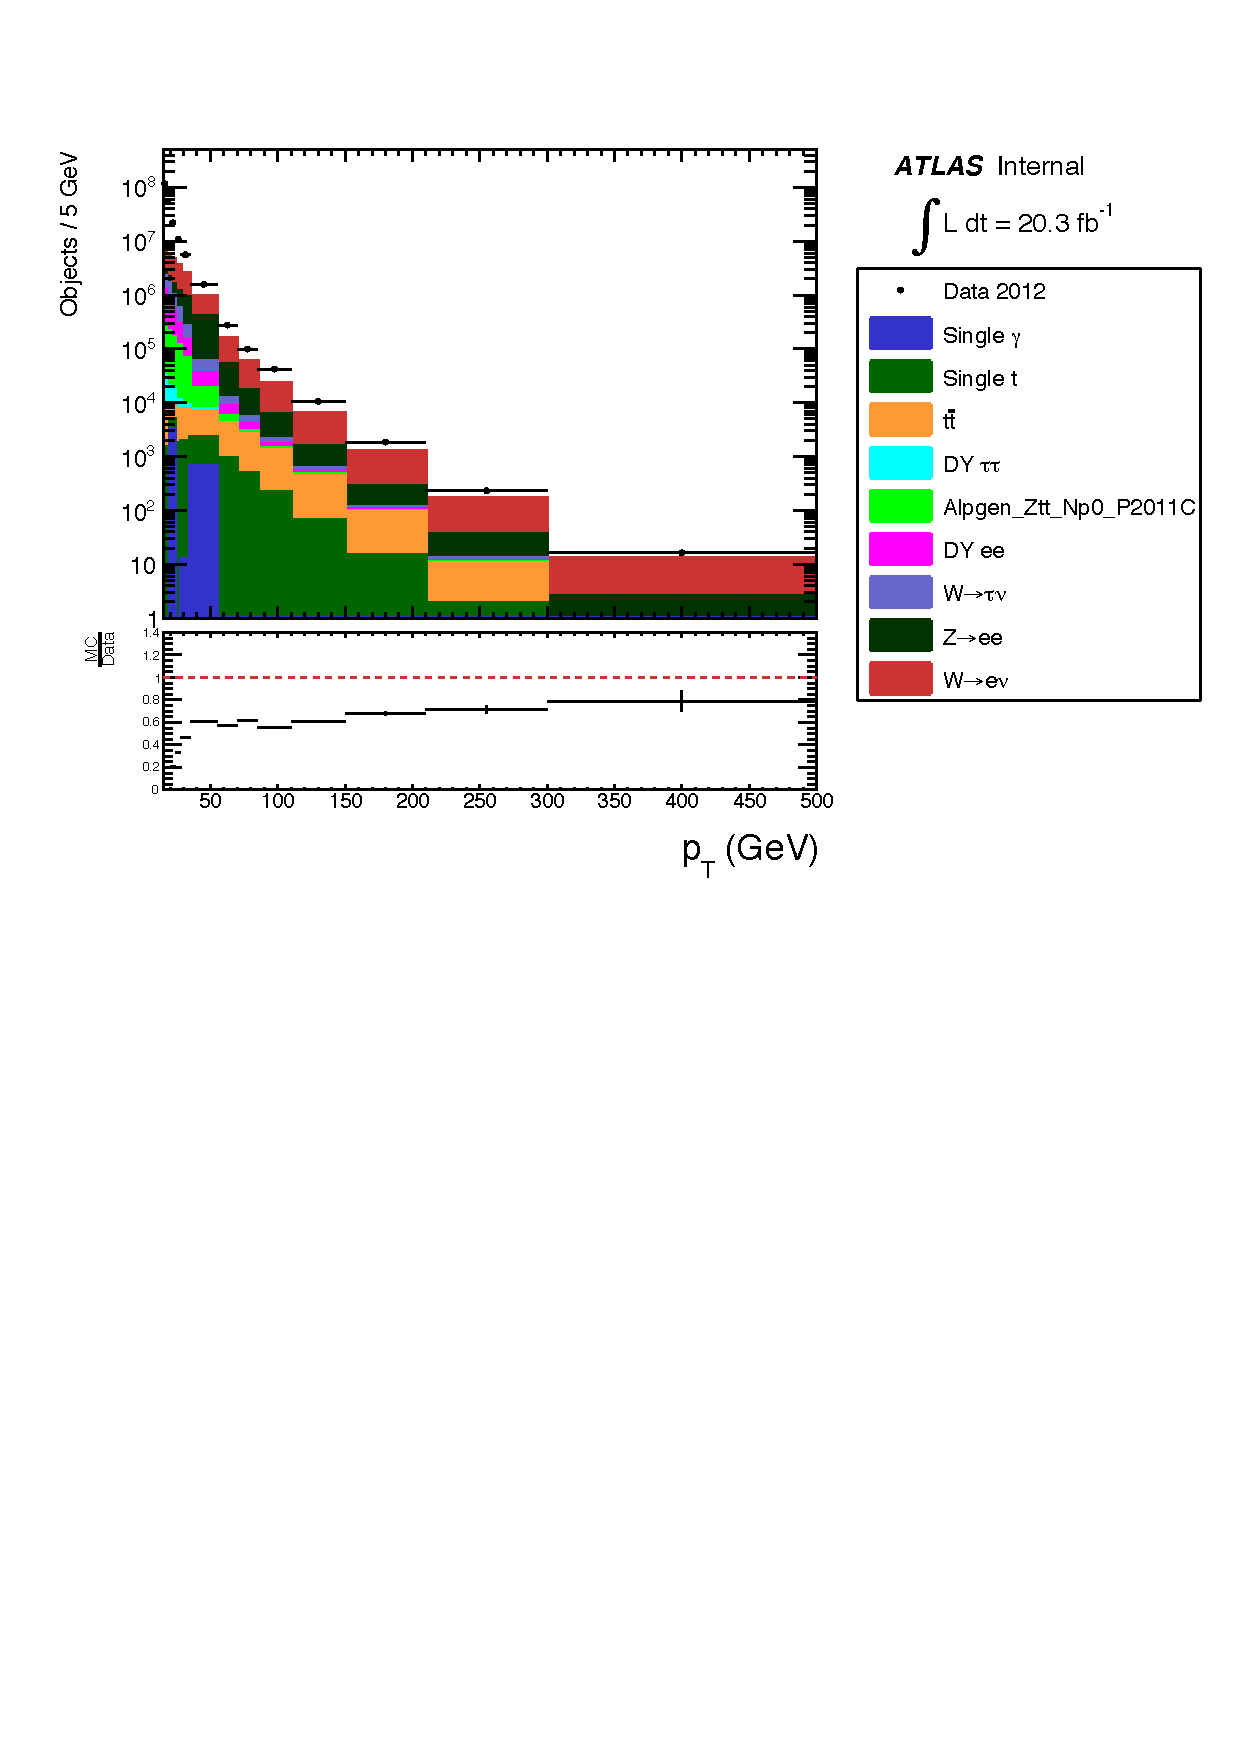
\includegraphics{figures/ch5-model-independent/c_ElectronNumerator_pt_log}}
	\label{f:numlogscale}
  }
  \subfloat[Denominators, log scale] {
	\resizebox{3in}{!}{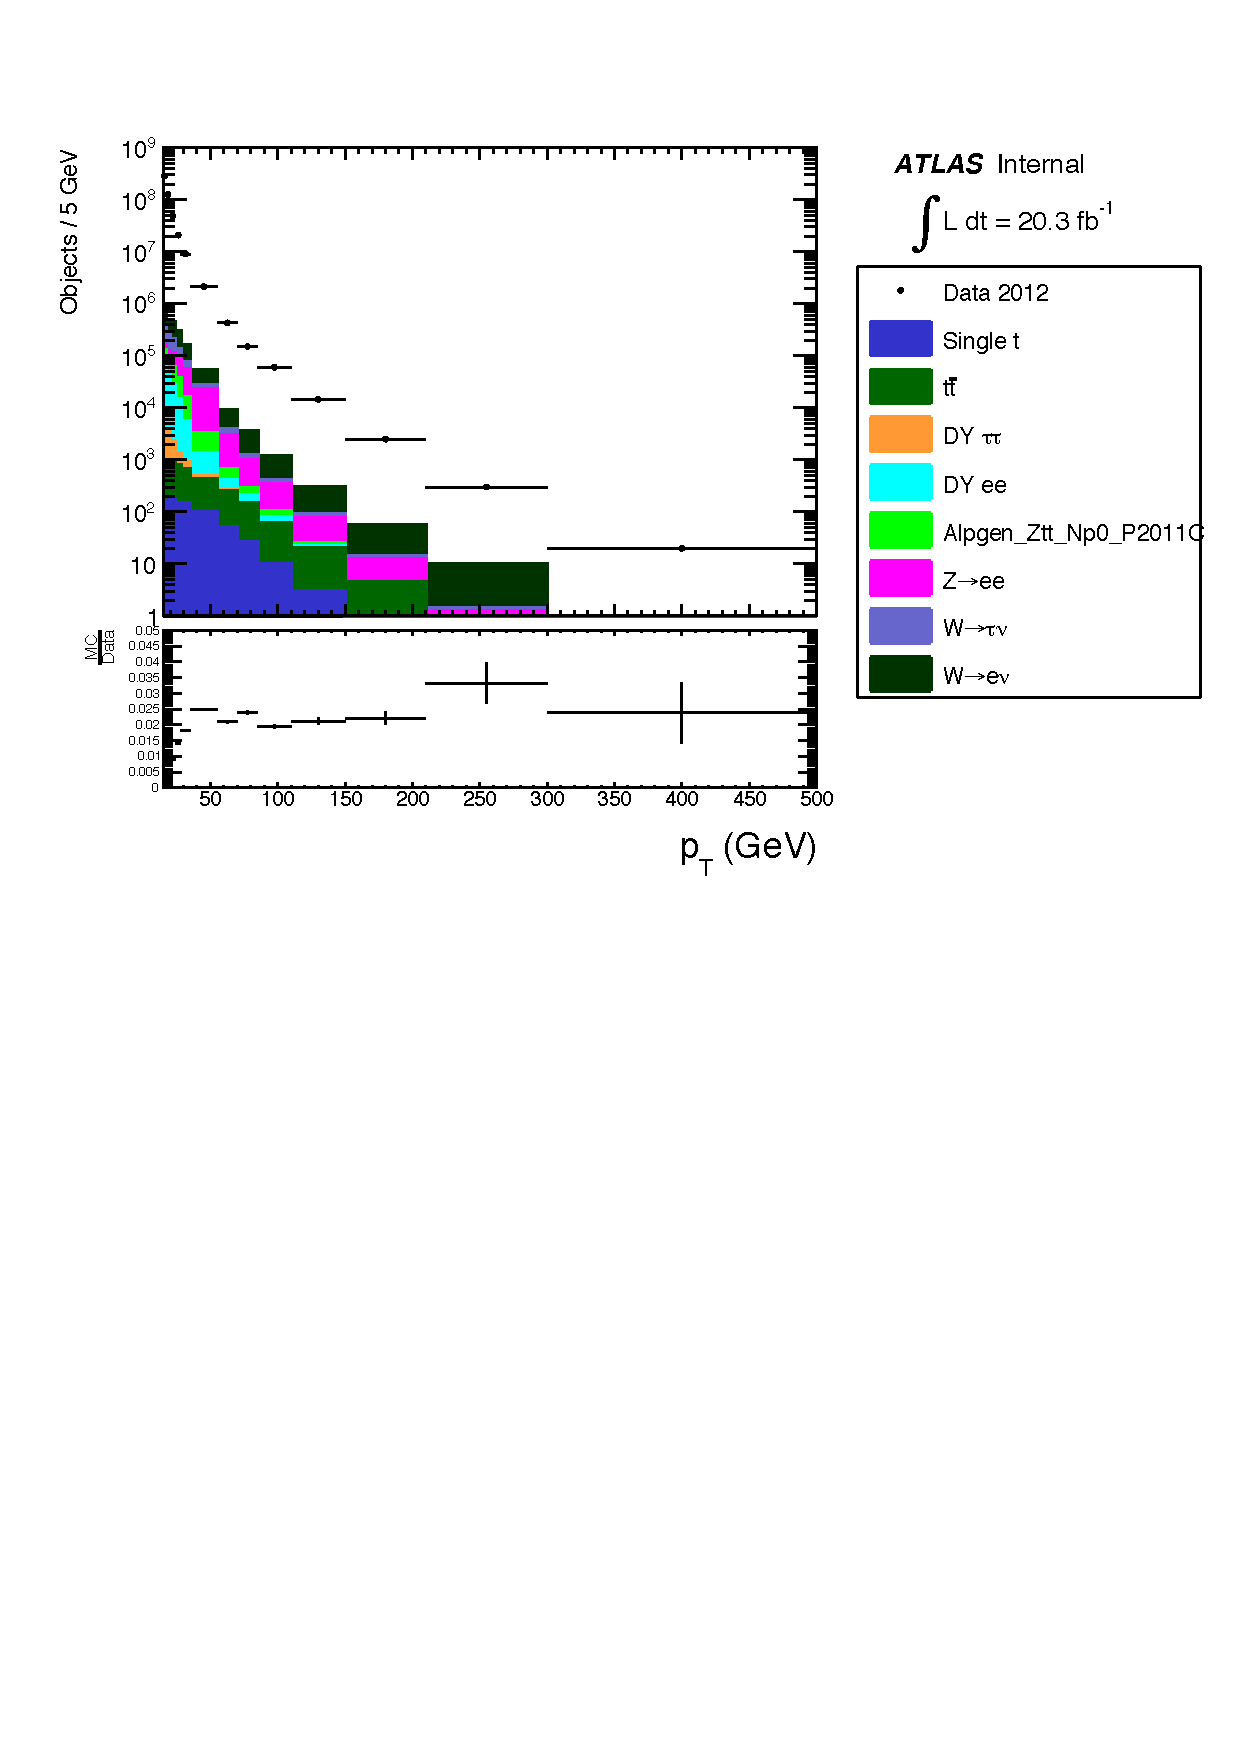
\includegraphics{figures/ch5-model-independent/c_ElectronDenominatorCombined_pt_log}}
	\label{f:denlogscale}
  } \\
  \subfloat[Numerators, linear scale] {
	\resizebox{3in}{!}{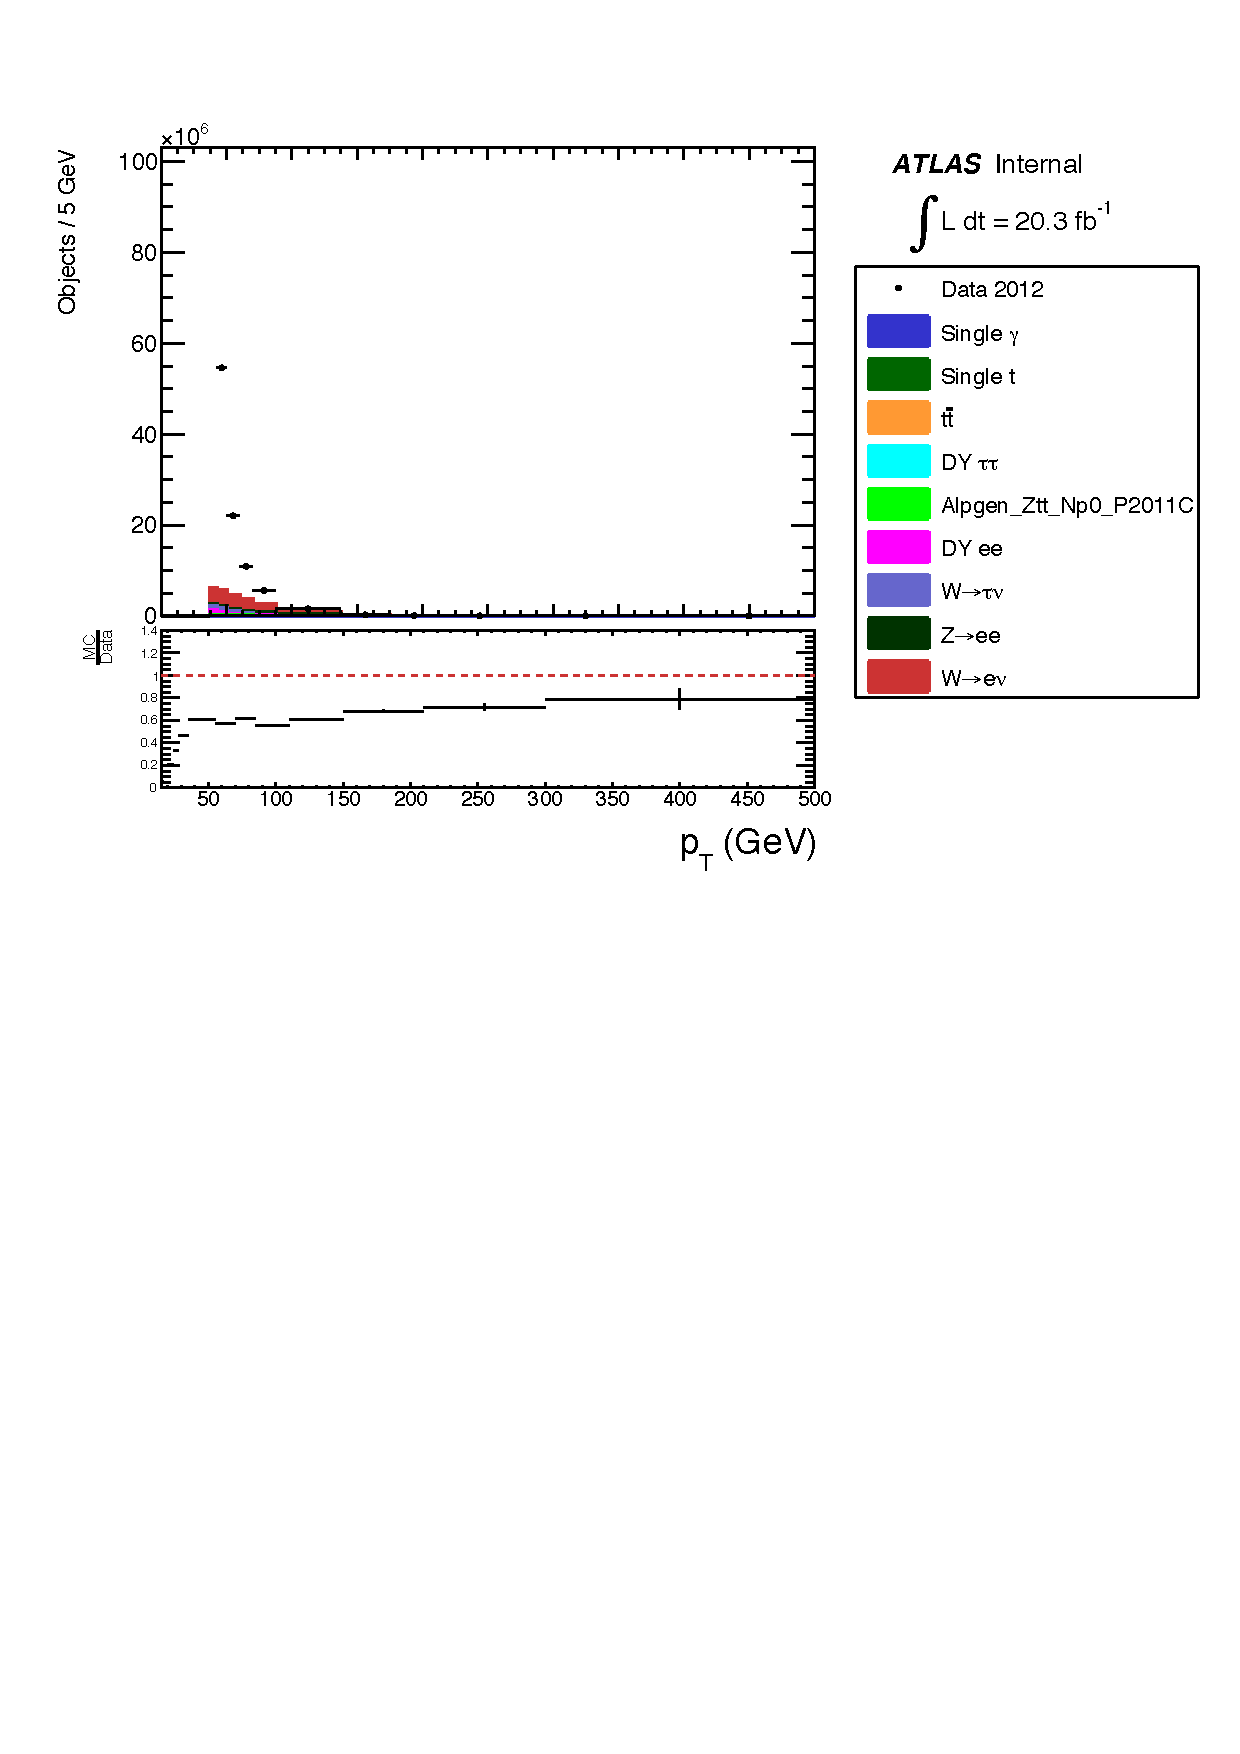
\includegraphics{figures/ch5-model-independent/c_ElectronNumerator_pt_linear}}
	\label{f:numlinscale}
  }
  \subfloat[Denominators, linear scale] {
	\resizebox{3in}{!}{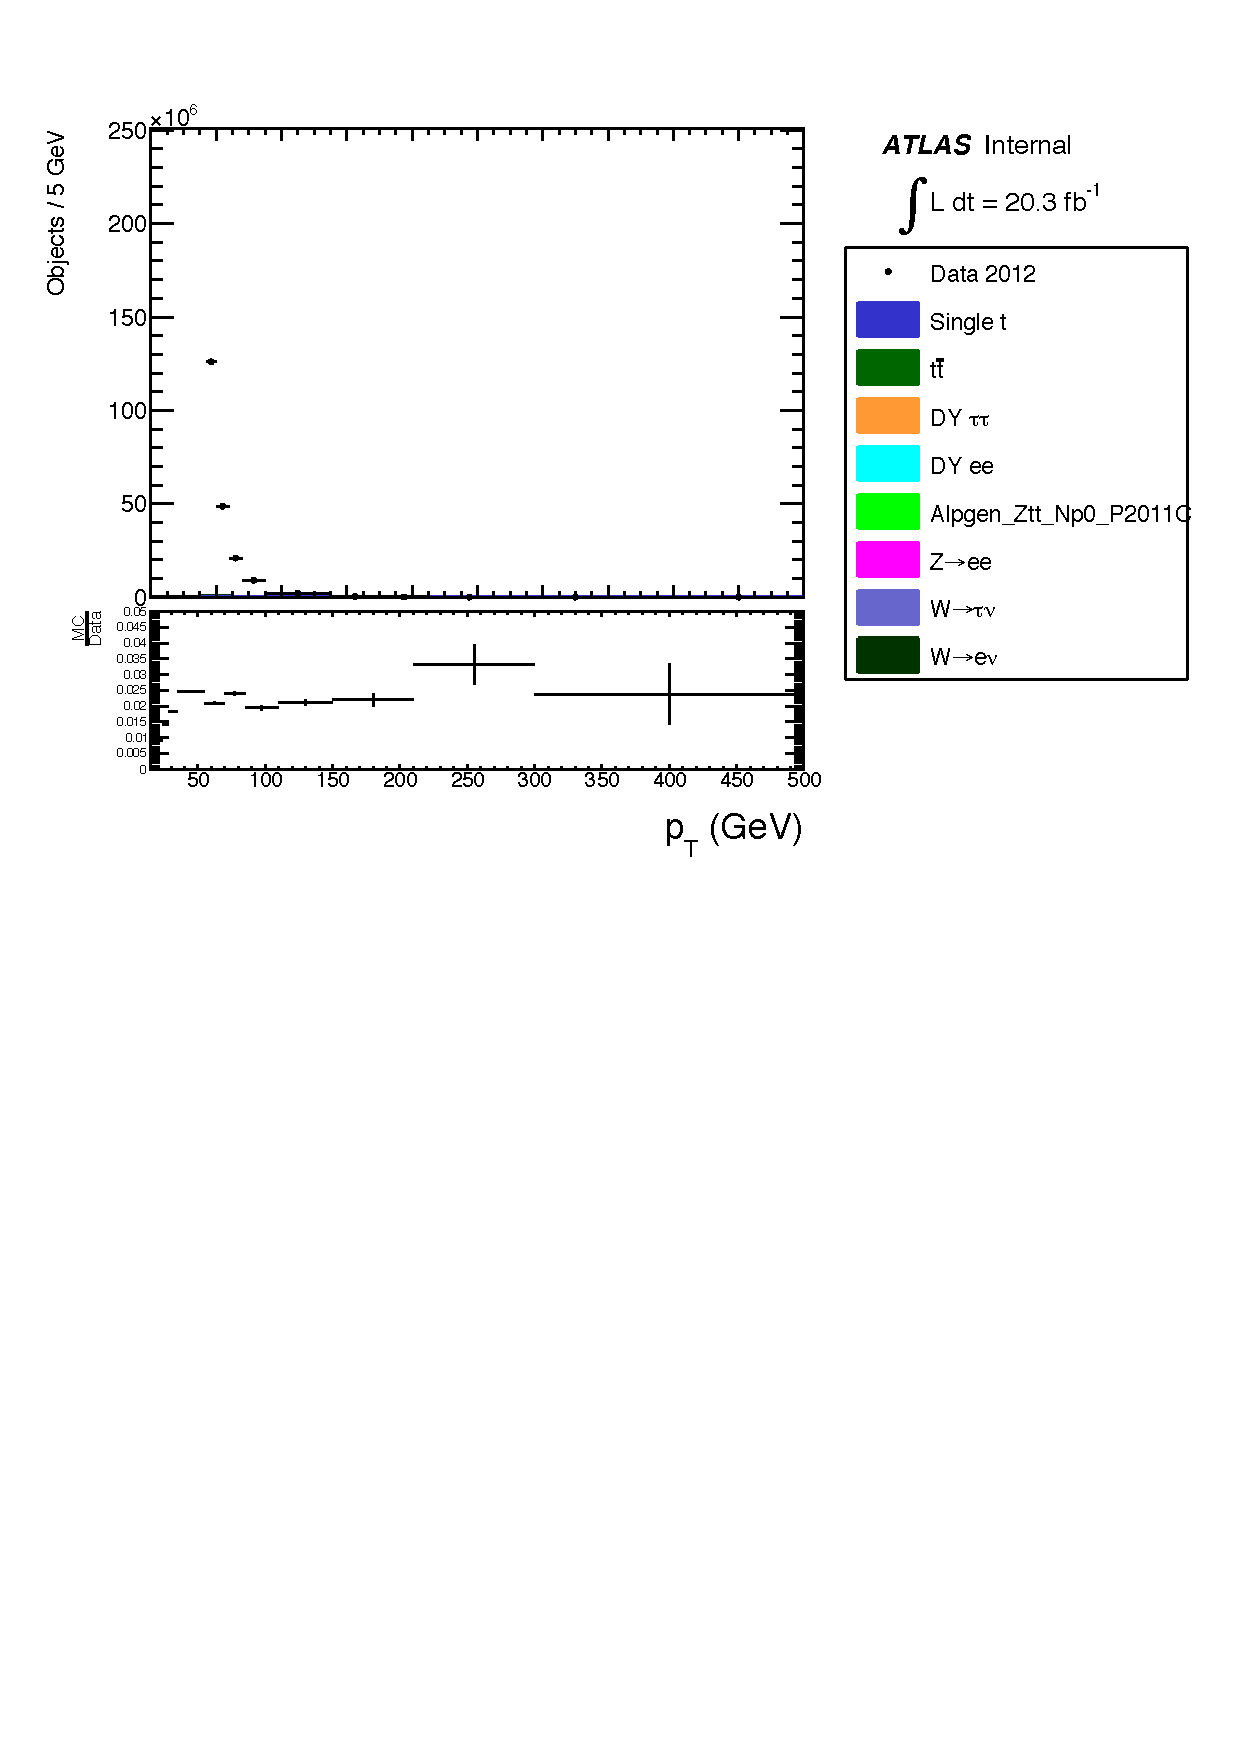
\includegraphics{figures/ch5-model-independent/c_ElectronDenominatorCombined_pt_linear}}
	\label{f:denlinscale}
  } \\
  \caption{Numerator and denominator electron object counts. The data sample consists of all single-electron events in the 2012 dataset, with cuts to reduce prompt contamination as described in the text. The markers represent object counts from 2012 data, and the colored histograms indicate the prompt subtractions estimated from Monte Carlo.}
  \label{fig:el-ff-data-prompt-subtractions}
\end{figure}

\begin{figure}[h]
  \centering
  \subfloat[Central values] {
	\resizebox{3in}{!}{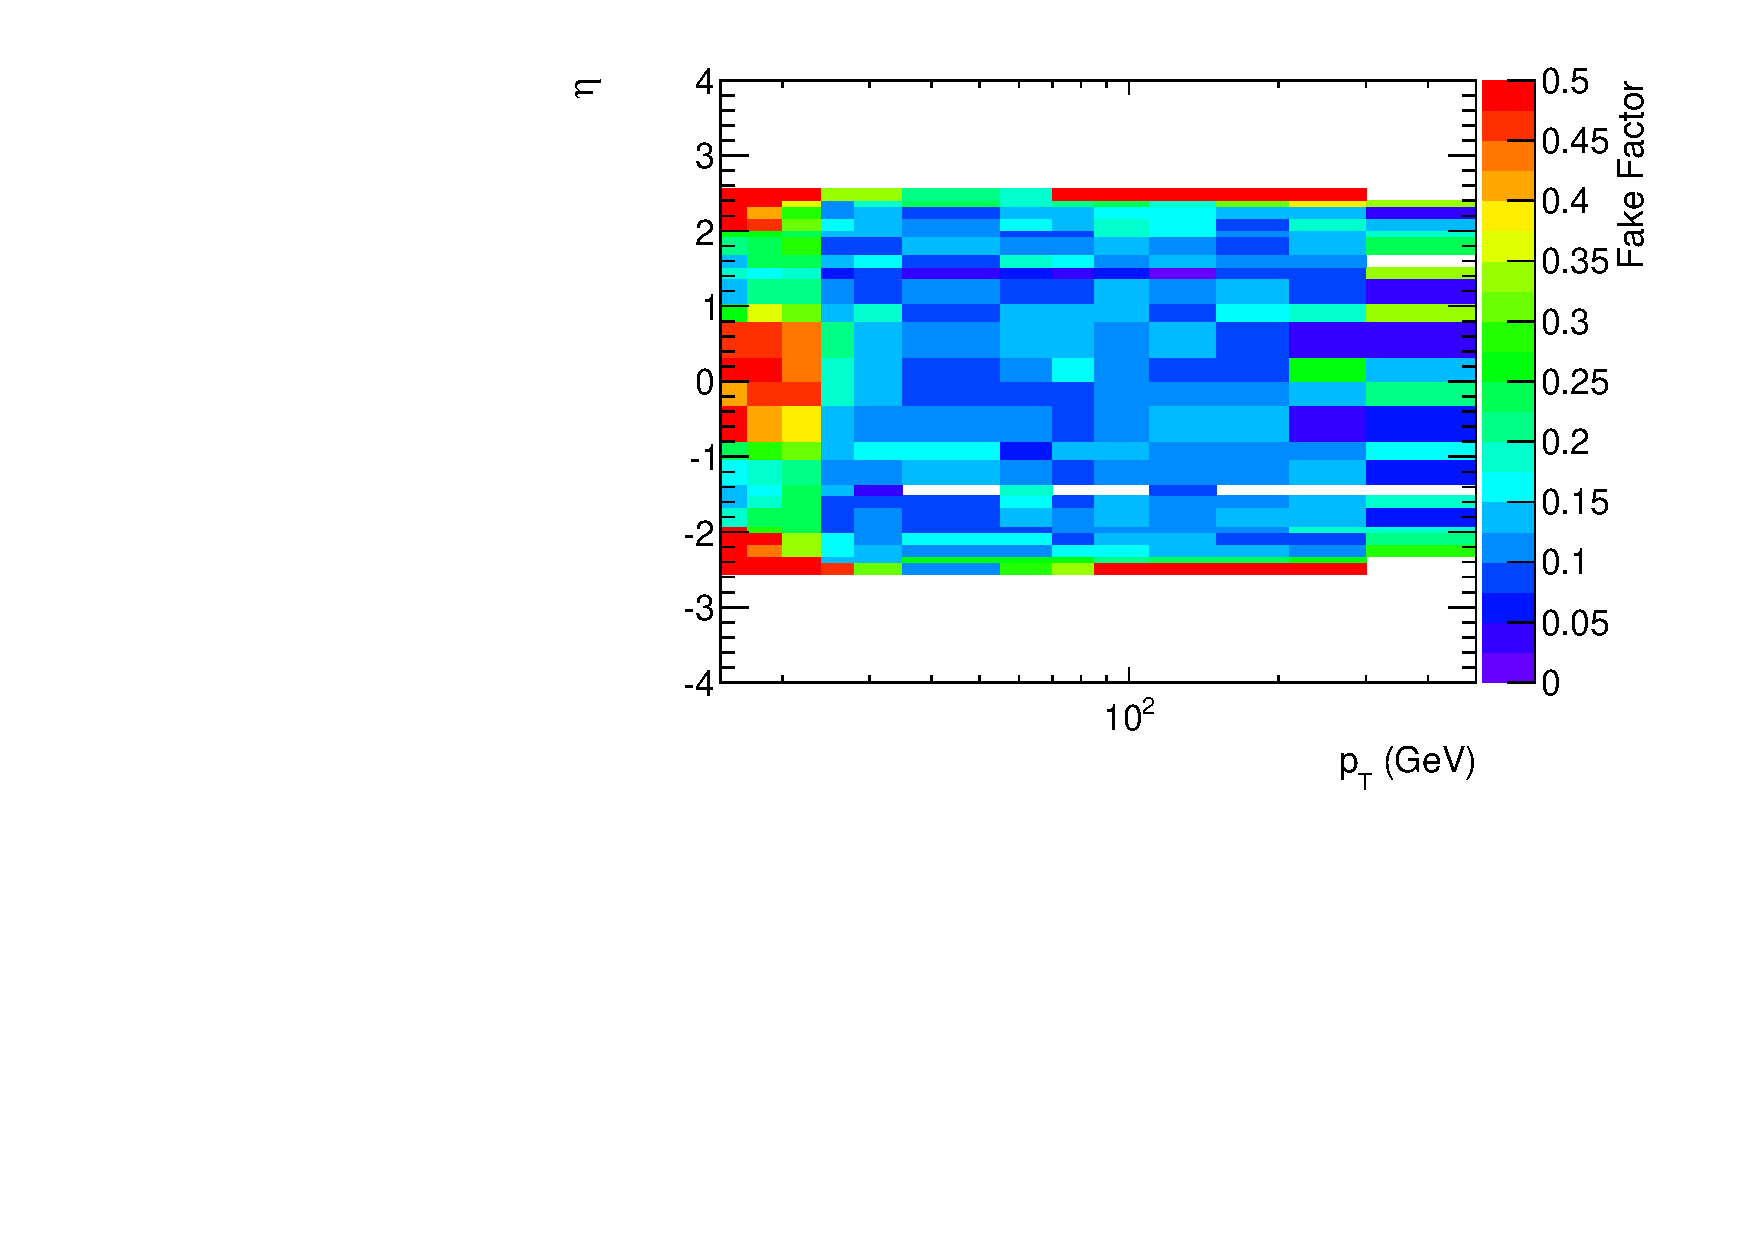
\includegraphics{figures/ch5-model-independent/c_FinalFF_2D}}
  }
  \subfloat[Statistical uncertainty over value] {
	\resizebox{3in}{!}{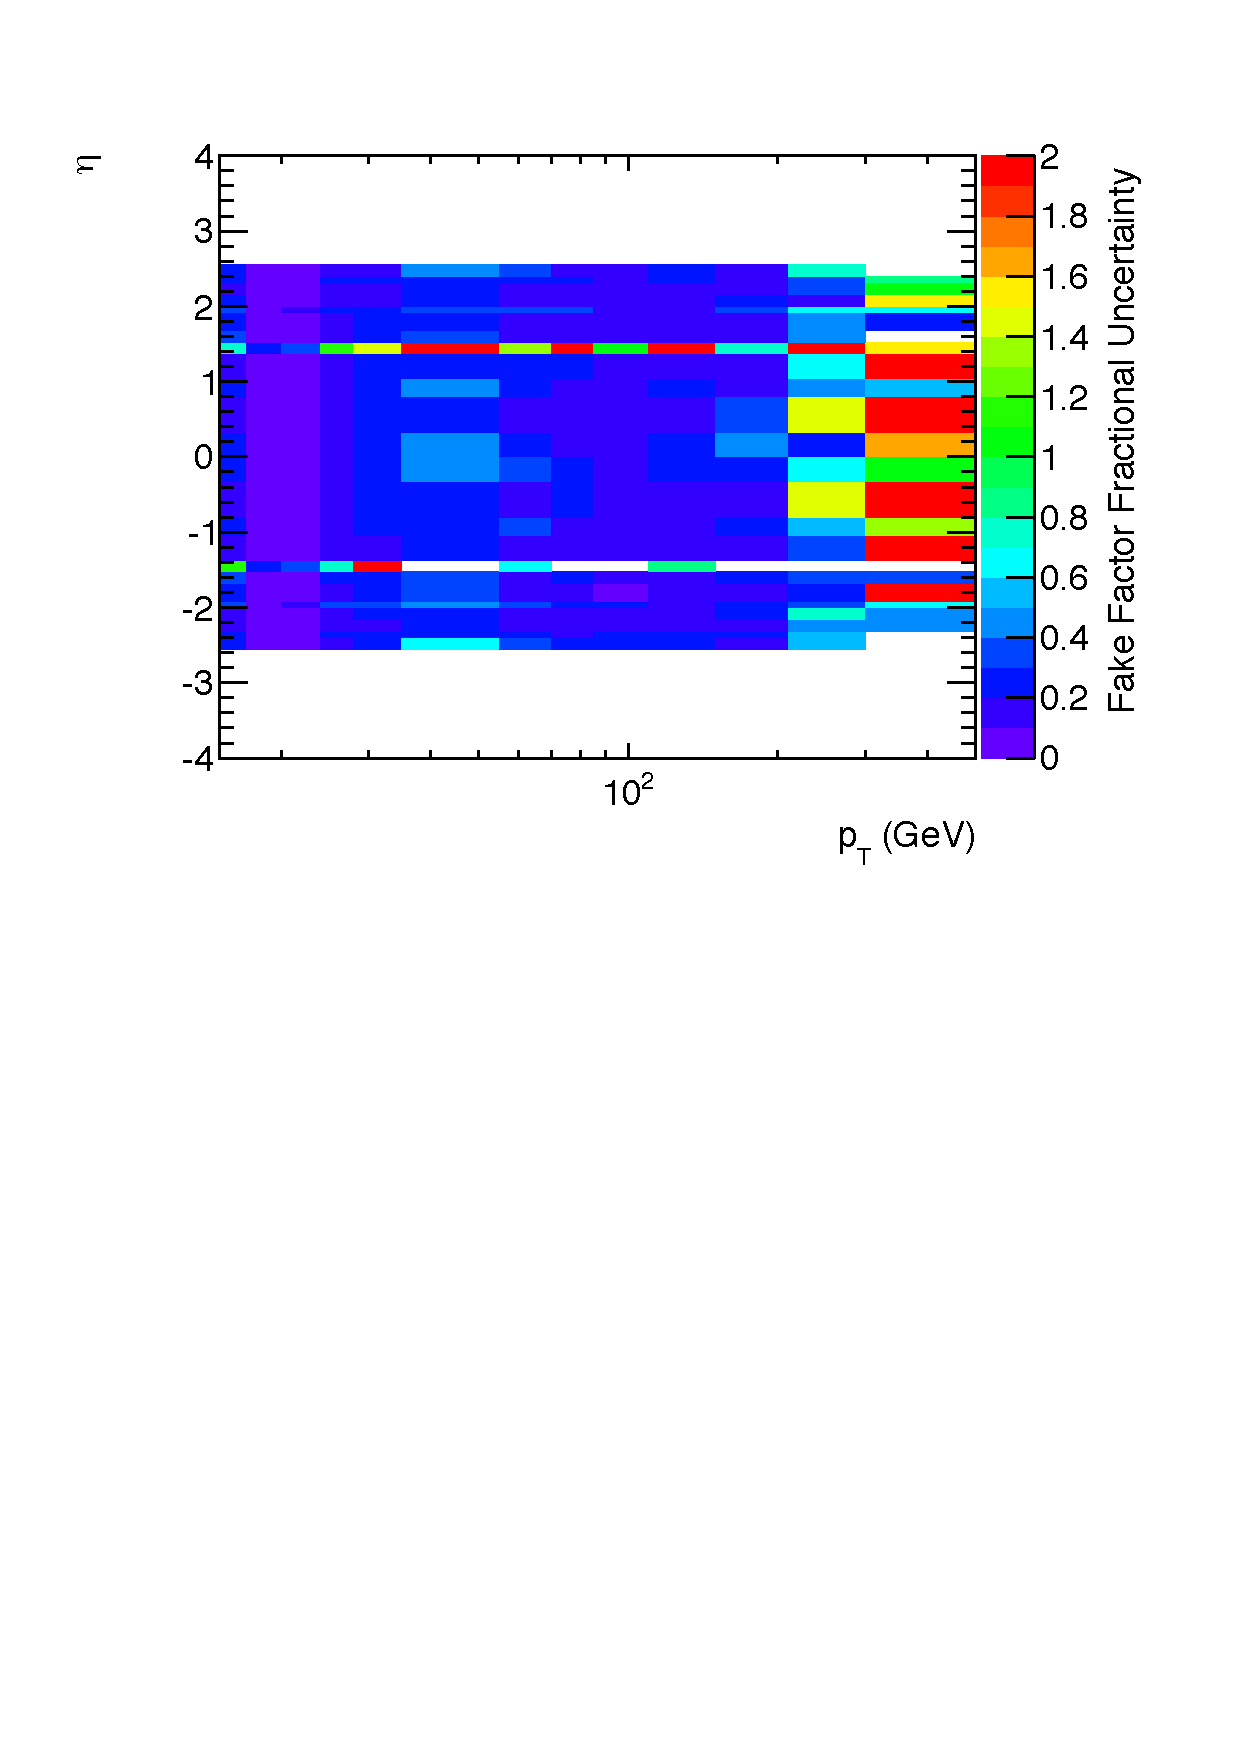
\includegraphics{figures/ch5-model-independent/c_FinalFF_2D_ErrorOverValue_corr}}
  }
  \caption{Electron fake factors parametrized in $p_T$ and $\eta$.}
  \label{fig:electron-fake-factor-values}
\end{figure}

\begin{figure}[h] 
  \centering
  \subfloat[Average fake factor vs. $p_{\mathrm{T}}$] {
	\resizebox{3in}{!}{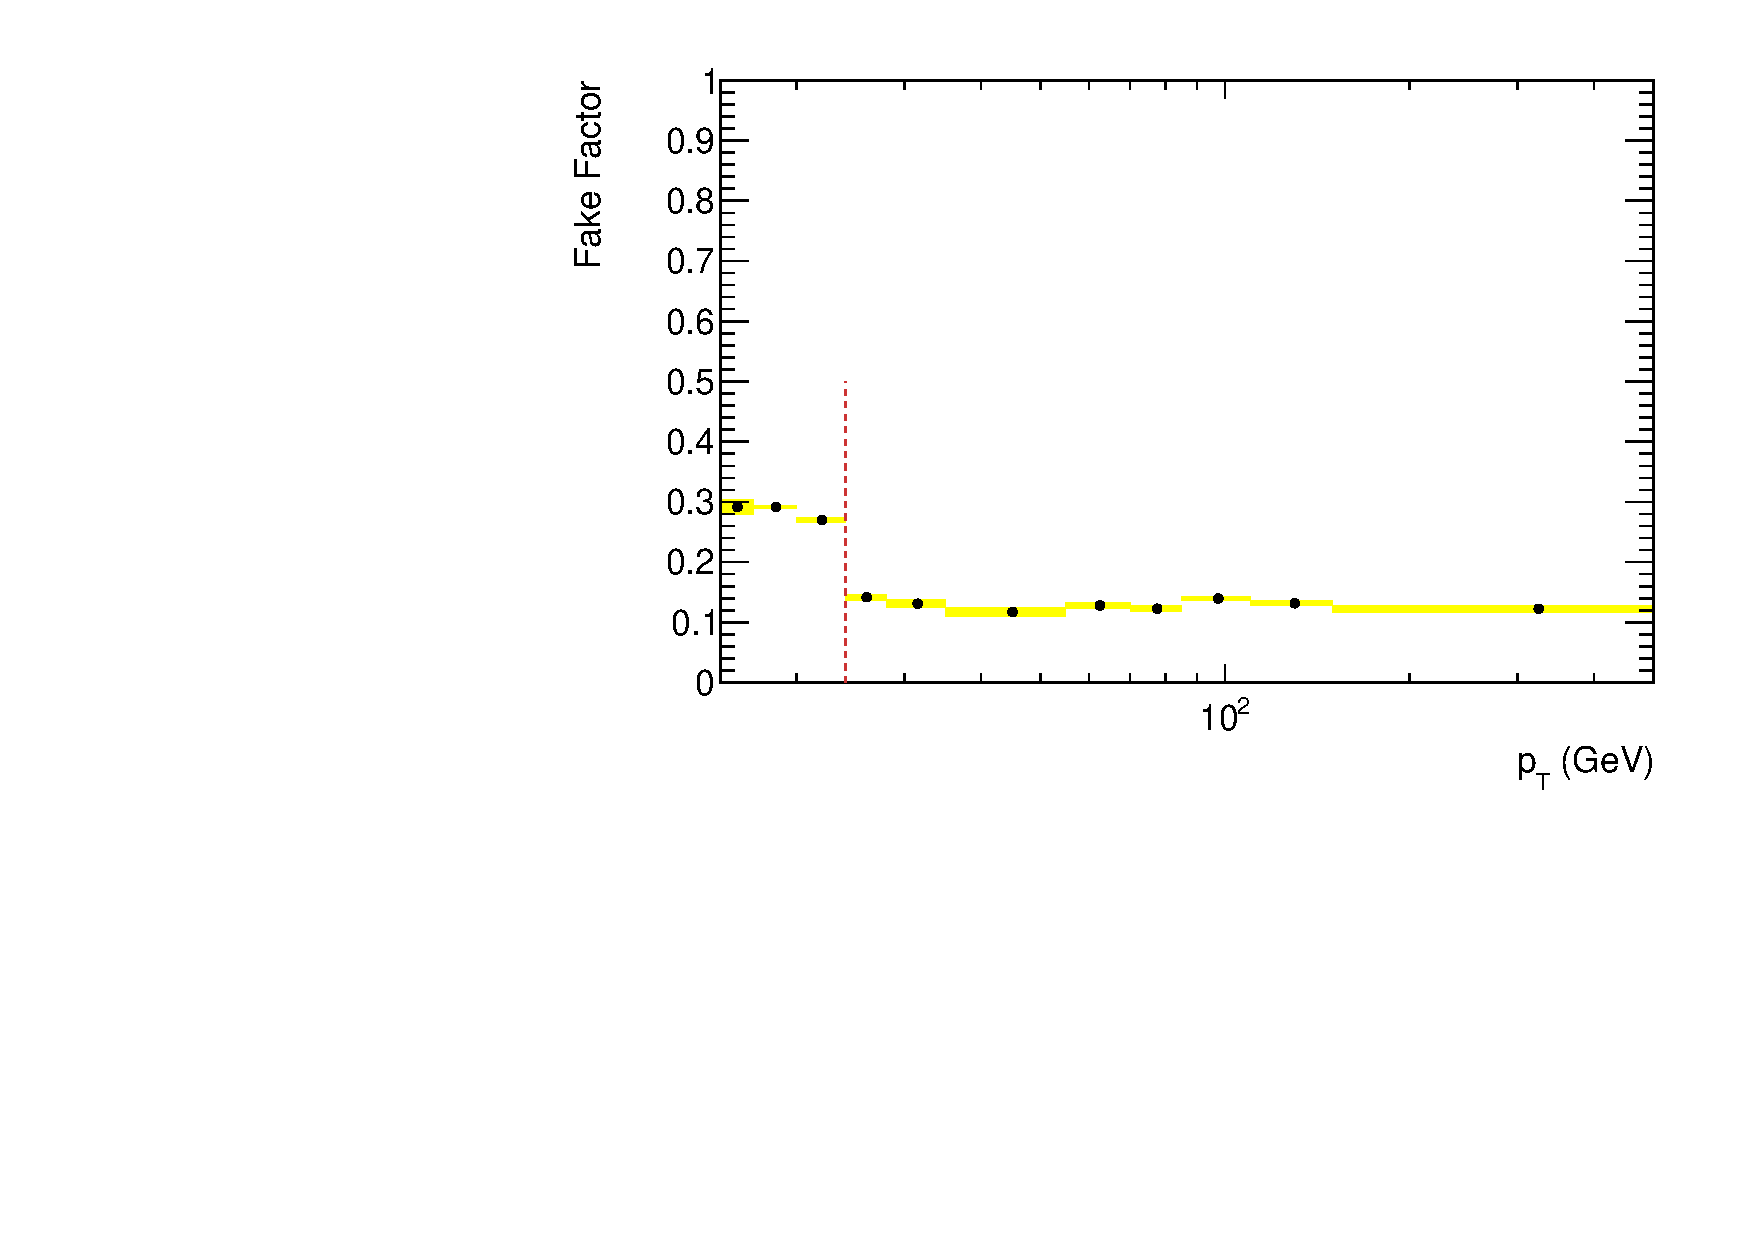
\includegraphics{figures/ch5-model-independent/c_FinalFF_1D_pt}}
  }
  \subfloat[Fake factors vs. $p_{\mathrm{T}}$ for different value of electron $|\eta|$] {
	\resizebox{3in}{!}{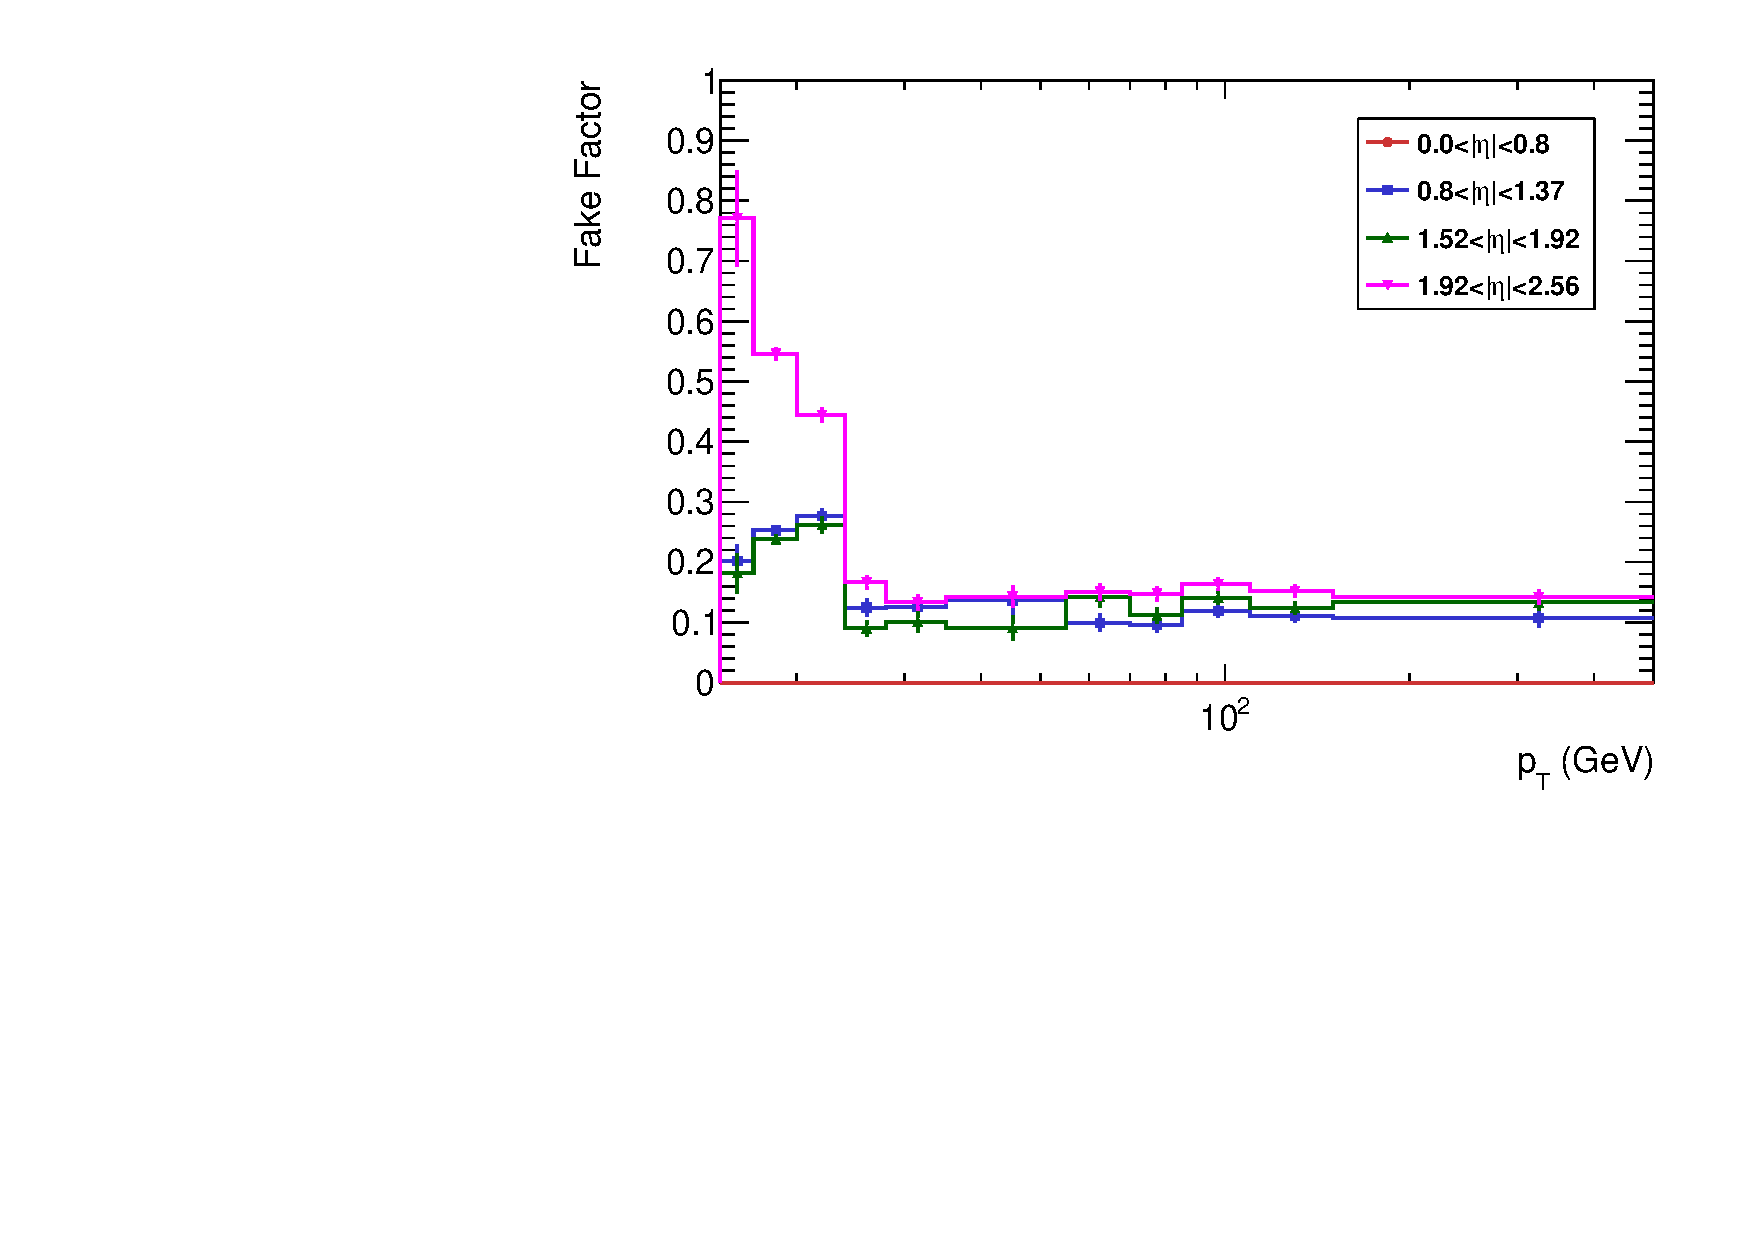
\includegraphics{figures/ch5-model-independent/c_FinalFF_1D_etaslices}}
  }
  \caption{Electron fake factors projected in $p_{\mathrm{T}}$. The denominator requirements are different below and above $24~\GeV$, where the triggers switch from EF\_eXX to EF\_gXX; below, the additional requirements on $\Delta\eta_1$ and $\Delta\phi_2$ cause a large drop in the denominators, and a large increase in the fake factor values.}
  \label{fig:electron-fake-factors-1D-pt}
\end{figure}

To help clarify the origin of the structure in $\eta$ observed at low $\pt$, the numerator and denominator counts are also shown versus $\eta$ for $\pt<24~\mbox{GeV}$ in figure~\ref{fig:electron-num-den-eta-lowpt}. The numerator counts are relative flat versus $\eta$ in the central region, and grow for $|\eta|\gtrsim 2$. Conversely, the denominators exhibit a significant increase near the barrel-endcap overlap region, and also for $|\eta|\gtrsim 2$. 

\begin{figure}[h]
  \centering
  \resizebox{5in}{!}{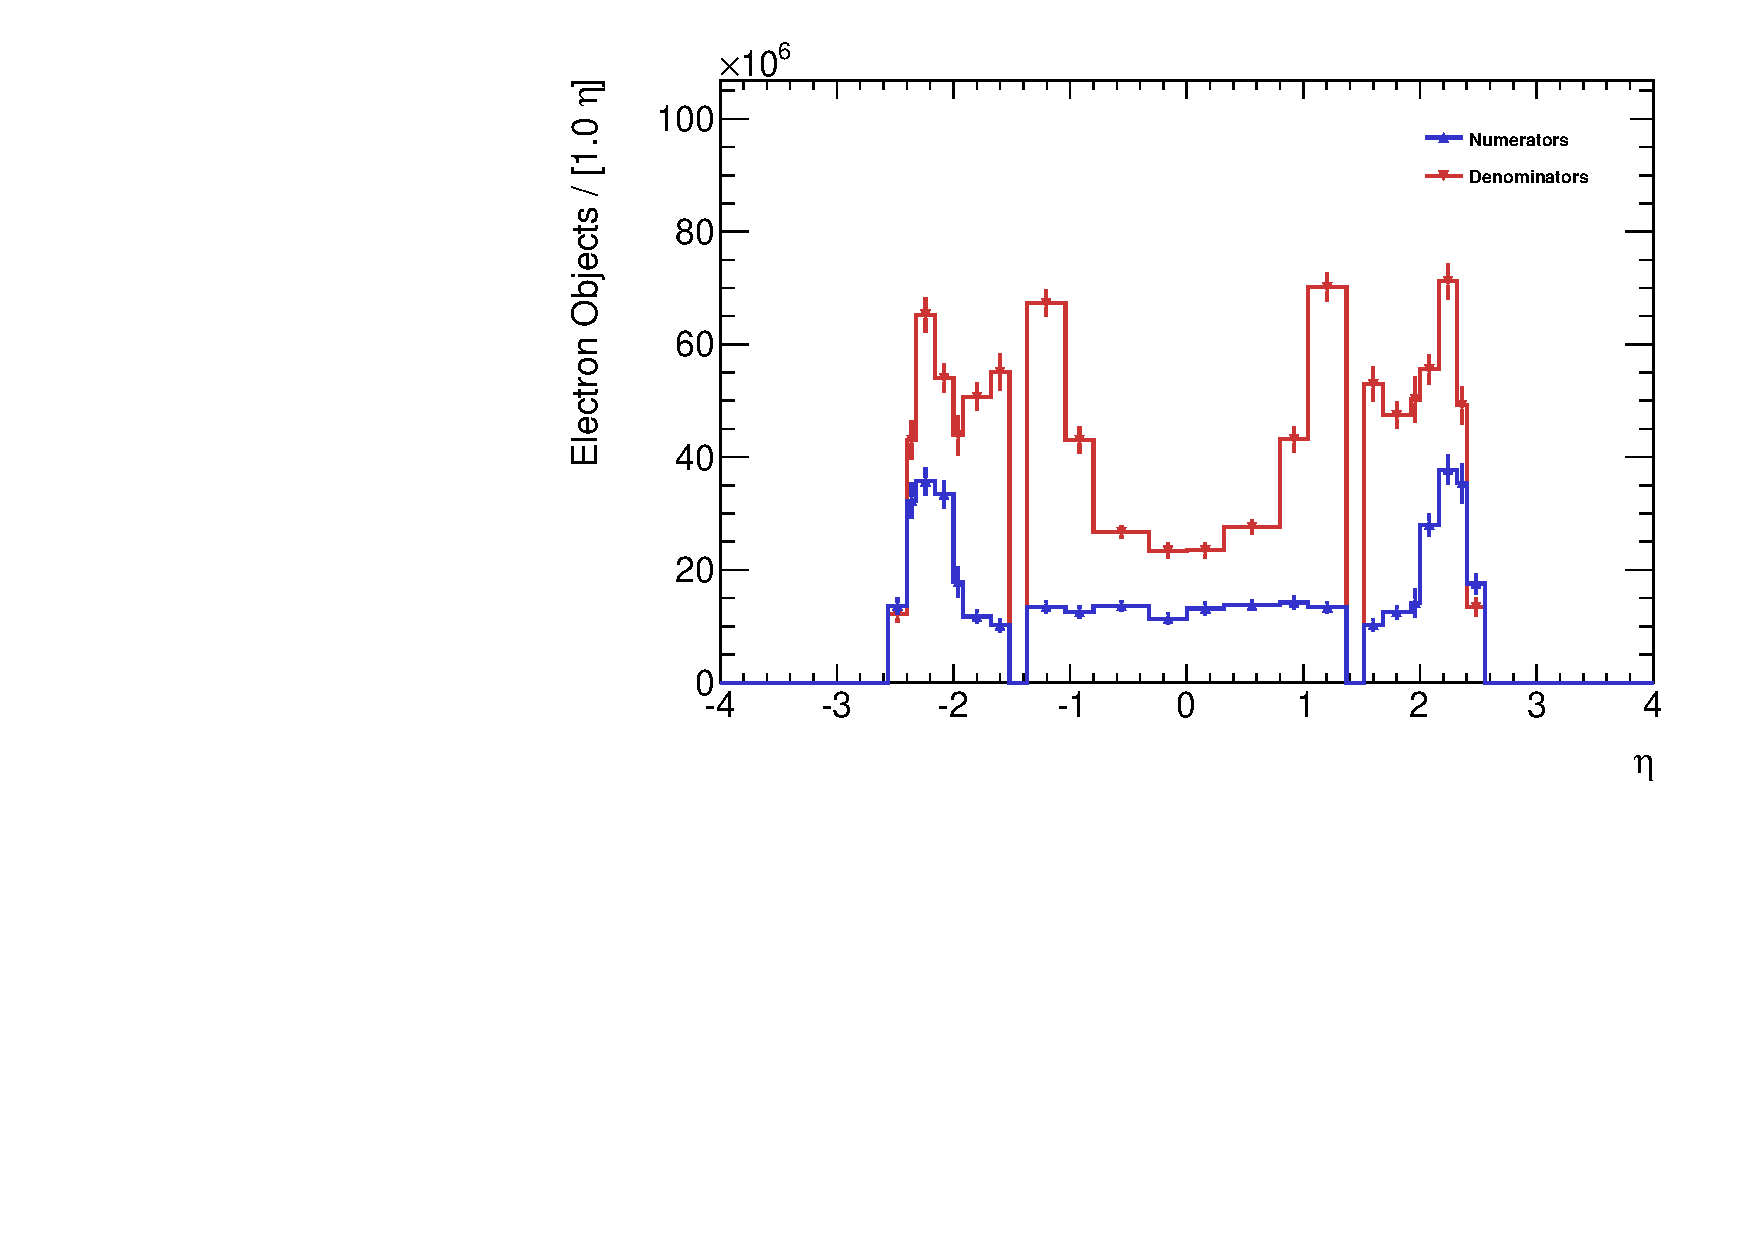
\includegraphics{figures/ch5-model-independent/c_NumDen_lowPt_eta}}
  \caption{Electron numerator and denominator object counts versus $\eta$ for $\pt<24~\mbox{GeV}$.}
  \label{fig:electron-num-den-eta-lowpt}
\end{figure}


The following sources of systematic uncertainty are considered. Again, we refer to~\cite{DeViveiros:1670929} for more details.
\begin{itemize}
  \item \textbf{Prompt subtraction}: The presence of real, prompt leptons from Standard Model processes in the sample used to measure the fake factors is accounted for using Monte Carlo simulation. Uncertainties on the simulated samples include luminosity; cross section uncertainties; and reconstruction, trigger, and identification efficiency scale factors. These lead to a maximum uncertainty of about $20\%$ where the prompt subtraction is largest. 
  \item \textbf{Trigger efficiency correction}: As mentioned previously, an inefficiency is observed in the loose electron triggers for offline \verb.loose++. electrons. This is due to the lack of GSF tracking in the trigger. For the fake factor derivation, this affects electrons in the range $15~\mbox{GeV}<\pt<24~\mbox{GeV}$, where photon triggers are not available. Imposing the \verb.tight++. cut on the track-cluster matching (the $\Delta \eta$ and $\Delta \phi$ between the electron track and calorimeter cluster) mitigates most, but not all, of the inefficiency, by cutting out electrons with large amounts of bremsstrahlung whose track are not reconstructed in the trigger. Based on a comparison of loose electron and photon triggers in the range $24~\mbox{GeV}<\pt<85~\mbox{GeV}$, a correction of about $8\%$ is applied to loose electron-triggererd events, and the same value is taken as systematic uncertainty.
  \item \textbf{Extrapolation to signal region}: Two systematic uncertainties are assigned to account for bias due to the extrapolation of fake factors from the control region to the signal region. First, the cuts on $m_{\mathrm{T}}$ and $\Etmiss$ are varied from $<40~\mbox{GeV}$ to $<25~\mbox{GeV}$ and $<55~\mbox{GeV}$. A $\pt$-dependent systematic uncertainty of up to $15\%$ is assigned. Second, Monte Carlo-based truth studies indicate that the fake factor values are quite different for heavy- and light-flavor jets, so a difference in heavy flavor fraction between the control and signal regions will bias the fake factors. The effect of this is estimated using a $t\overline{t}$ Monte Carlo sample, and a flat systematic uncertainty of $20\%$ is assigned. See appendix~\ref{sec:appendix-el-ff-hflf-syst} for more information.
\end{itemize}
The systematic and total uncertainties on the fake factors are shown as a function of $\pt$ in figure~\ref{fig:electron-fake-factor-uncertainties}.

\begin{figure}[h] 
  \centering
  \subfloat[Linear scale] {
	\resizebox{3in}{!}{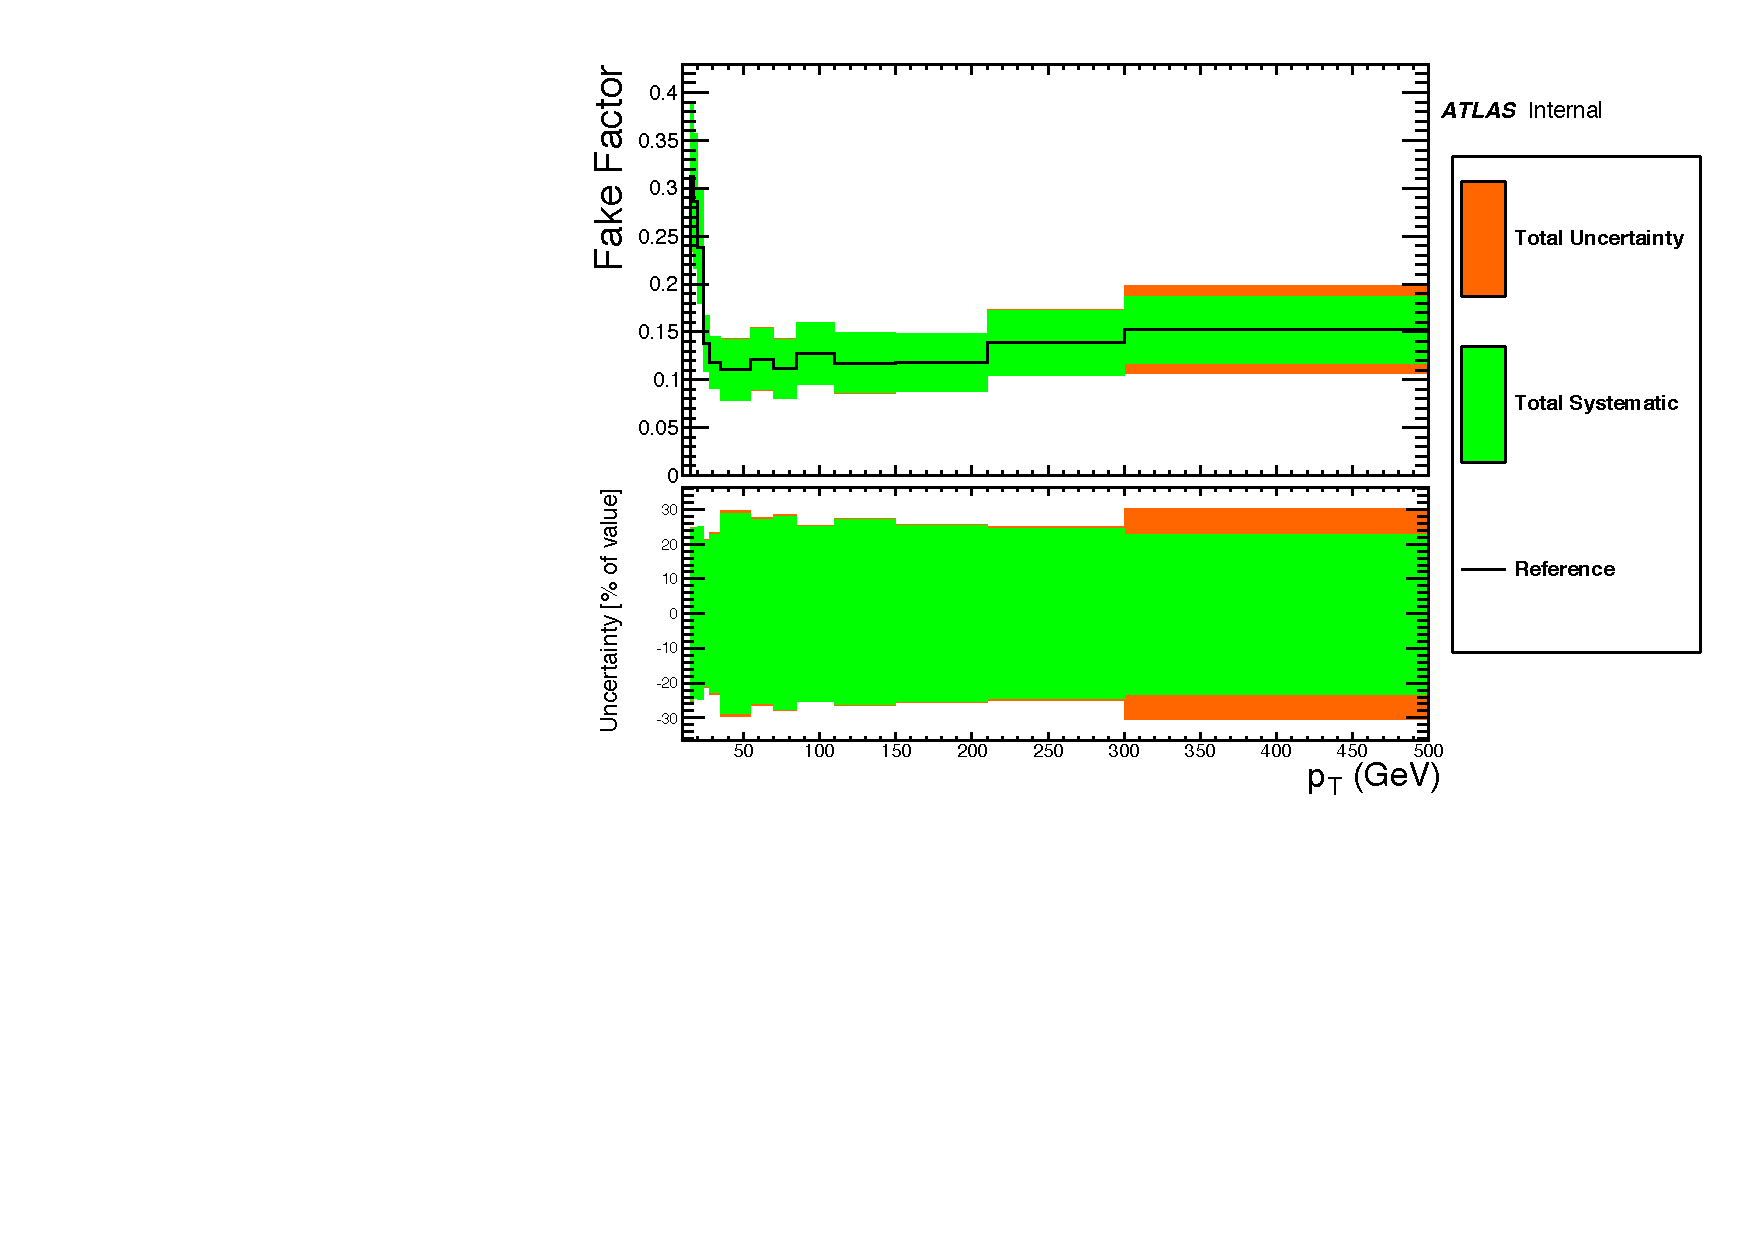
\includegraphics{figures/ch5-model-independent/c_FinalFF_systematics_linearx_biggerlabels}}
  }
  \subfloat[Log scale] {
	\resizebox{3in}{!}{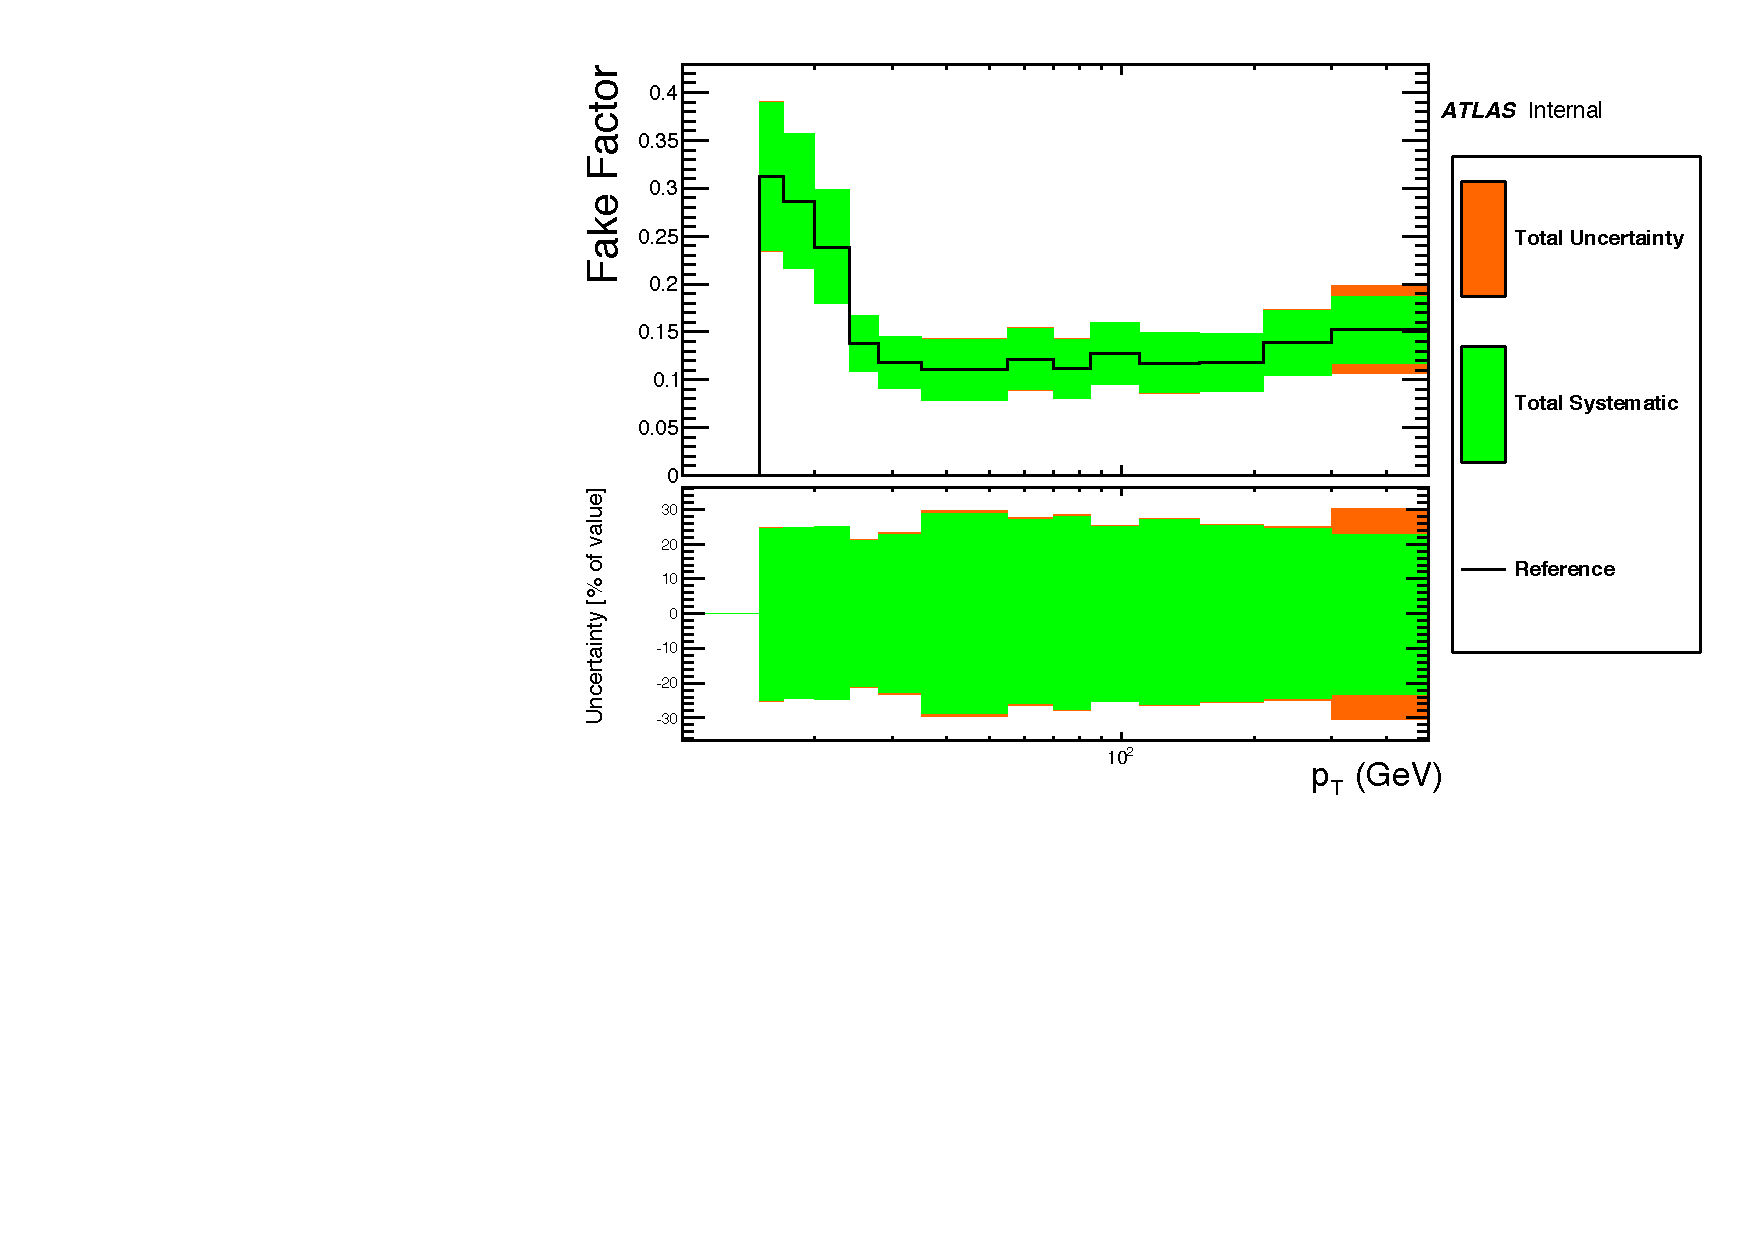
\includegraphics{figures/ch5-model-independent/c_FinalFF_systematics_logx_biggerlabels}}
  }
  \caption{Electron fake factors vs. $\pt$ with systematic and total uncertainties. The statistical uncertainty includes both the data and prompt subtraction Monte Carlo statistics.}
  \label{fig:electron-fake-factor-uncertainties}
\end{figure}

\clearpage

\subsubsection{Muon Fake Factors}\label{sec:muon-fake-factors}
The muon fake factor method follows that used in the same-sign dilepton search in 2011~\cite{LouiseThesis, 
SSInternal}. The method targets non-prompt muons from semileptonic heavy flavor decays, punch-through, and decays-in-flight of long-lived mesons by inverting the isolation requirements. Specifically, the denominator muons are defined as follows:
\begin{itemize}
  \item Pass all numerator muon requirements in table~\ref{table:lepton-selections}, except the requirements on \verb.Etcone30., \verb.ptcone30., and $\frac{d_0}{\sigma_{d_0}}$. 
  \item Loosen impact parameter cut:
  \begin{equation}
	|\frac{d_0}{\sigma_{d_0}}|<10
  \end{equation}
  \item Invert isolation:
  \begin{align}
	\etcones{30},\ \ptcones{30} &> \left\{\begin{array}{ccc} 0.15 \pt & : & \pt<100~\mbox{GeV} \\ 15+0.01 \pt~\mbox{GeV} & : & \pt>100~\mbox{GeV} \end{array} \right. \\
	\etcone{30} &< 2.0 \\
	\ptcone{30} &< 2.0 \\
  \end{align}
  \item If $\pt<40~\mbox{GeV}$, apply the same overlap requirement as the signal regions, removing the muon if $\Delta R (\mu,\ \mbox{jet})<0.3$. This overlap requirement is not applied for muons with $\pt>40~\mbox{GeV}$, which increases the statistical precision at the expense of additional systematic uncertainty. This is denoted by ``dR'' or ``non-dR'' below, for example in figure~\ref{fig:MuFake_ff_1D}.
\end{itemize}

The muon fake factors are measured in a same-sign dimuon sample, triggered by the \verb.EF_2mu13. trigger. The use of same-sign muons suppresses the prompt contamination from $Z/\gamma^{*}$ events. The measurement uses only muons with large track impact parameter significance, $|\frac{d_0}{\sigma_{d_0}}|>3$, to obtain a sample enriched in non-prompt muons (if both muons satisfy this requirement, then both are counted in the measurement). An extrapolation factor is derived from Monte Carlo to account for the fact that the signal region requires $|\frac{d_0}{\sigma_{d_0}}|<3$, as detailed below.

Two sets of fake factors are measured, depending on the jet activity in the event. In the following, jets are required to have $\pt>30~\mbox{GeV}$, and be separated from muons with $\Delta R(\mu,\ \mbox{jet})>0.3$. 
\begin{itemize}
  \item \textbf{Inclusive}: Applied to events with zero jets. The measurement uses the entire same-sign dimuon sample.
  \item \textbf{Two-Jet}: Applied to events with one or more jet. The measurement uses same-sign dimuon events with at least two jets with $\pt>30~\mbox{GeV}$. 
\end{itemize}
Fake muons from the two-jet sample are expected to come primarily from $W+\mbox{jets}$ and $t\overline{t}$ processes, while the inclusive sample also includes contributions from $b\overline{b}$. Figure~\ref{fig:MuFake_stacks} shows the $\pt$ distributions of numerator and denominator muons in the measurement sample along with the expected prompt
contributions. 
\begin{figure}[h]
  \subfloat[Numerators, 0-jet]{
	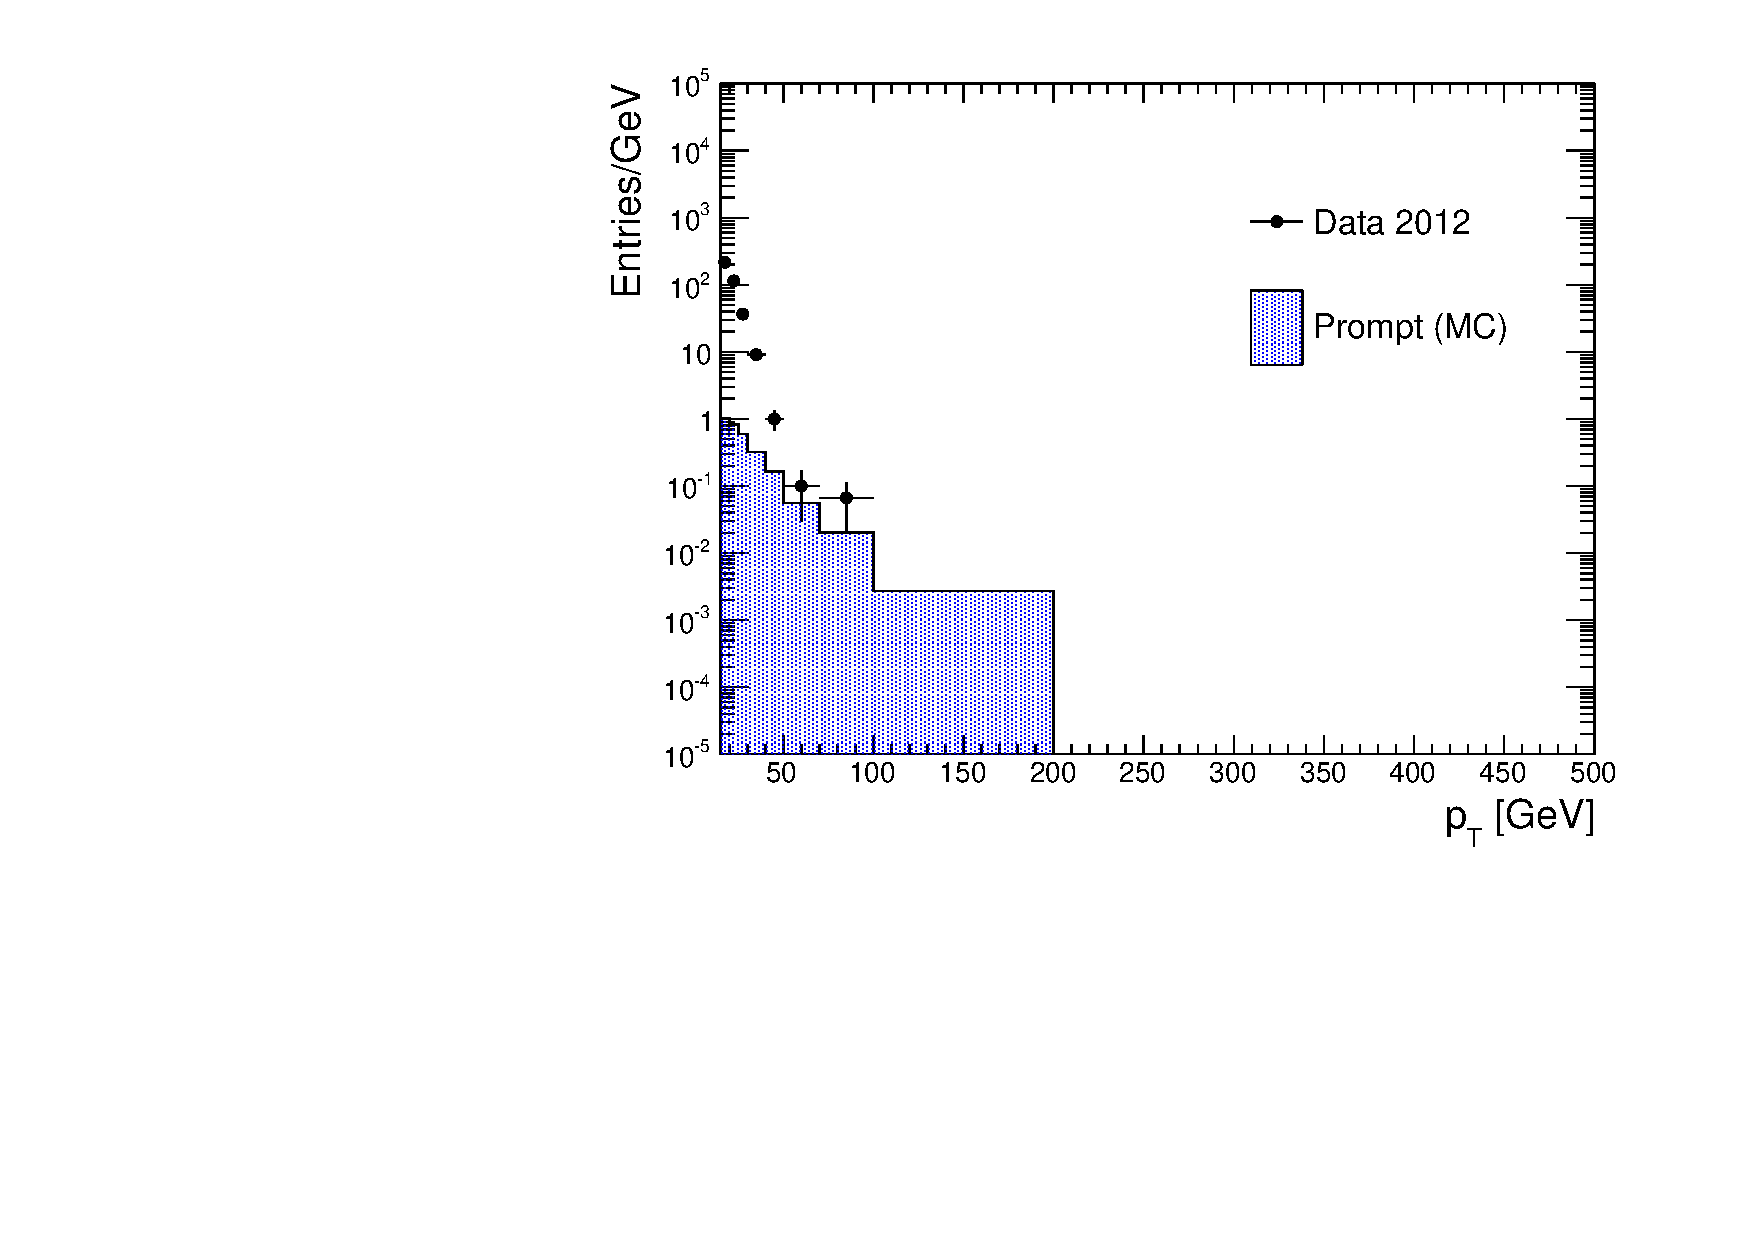
\includegraphics[width=0.3\columnwidth]{figures/ch5-model-independent/num__0jet__nodr}
  }
  \subfloat[Numerators, 1-jet]{
	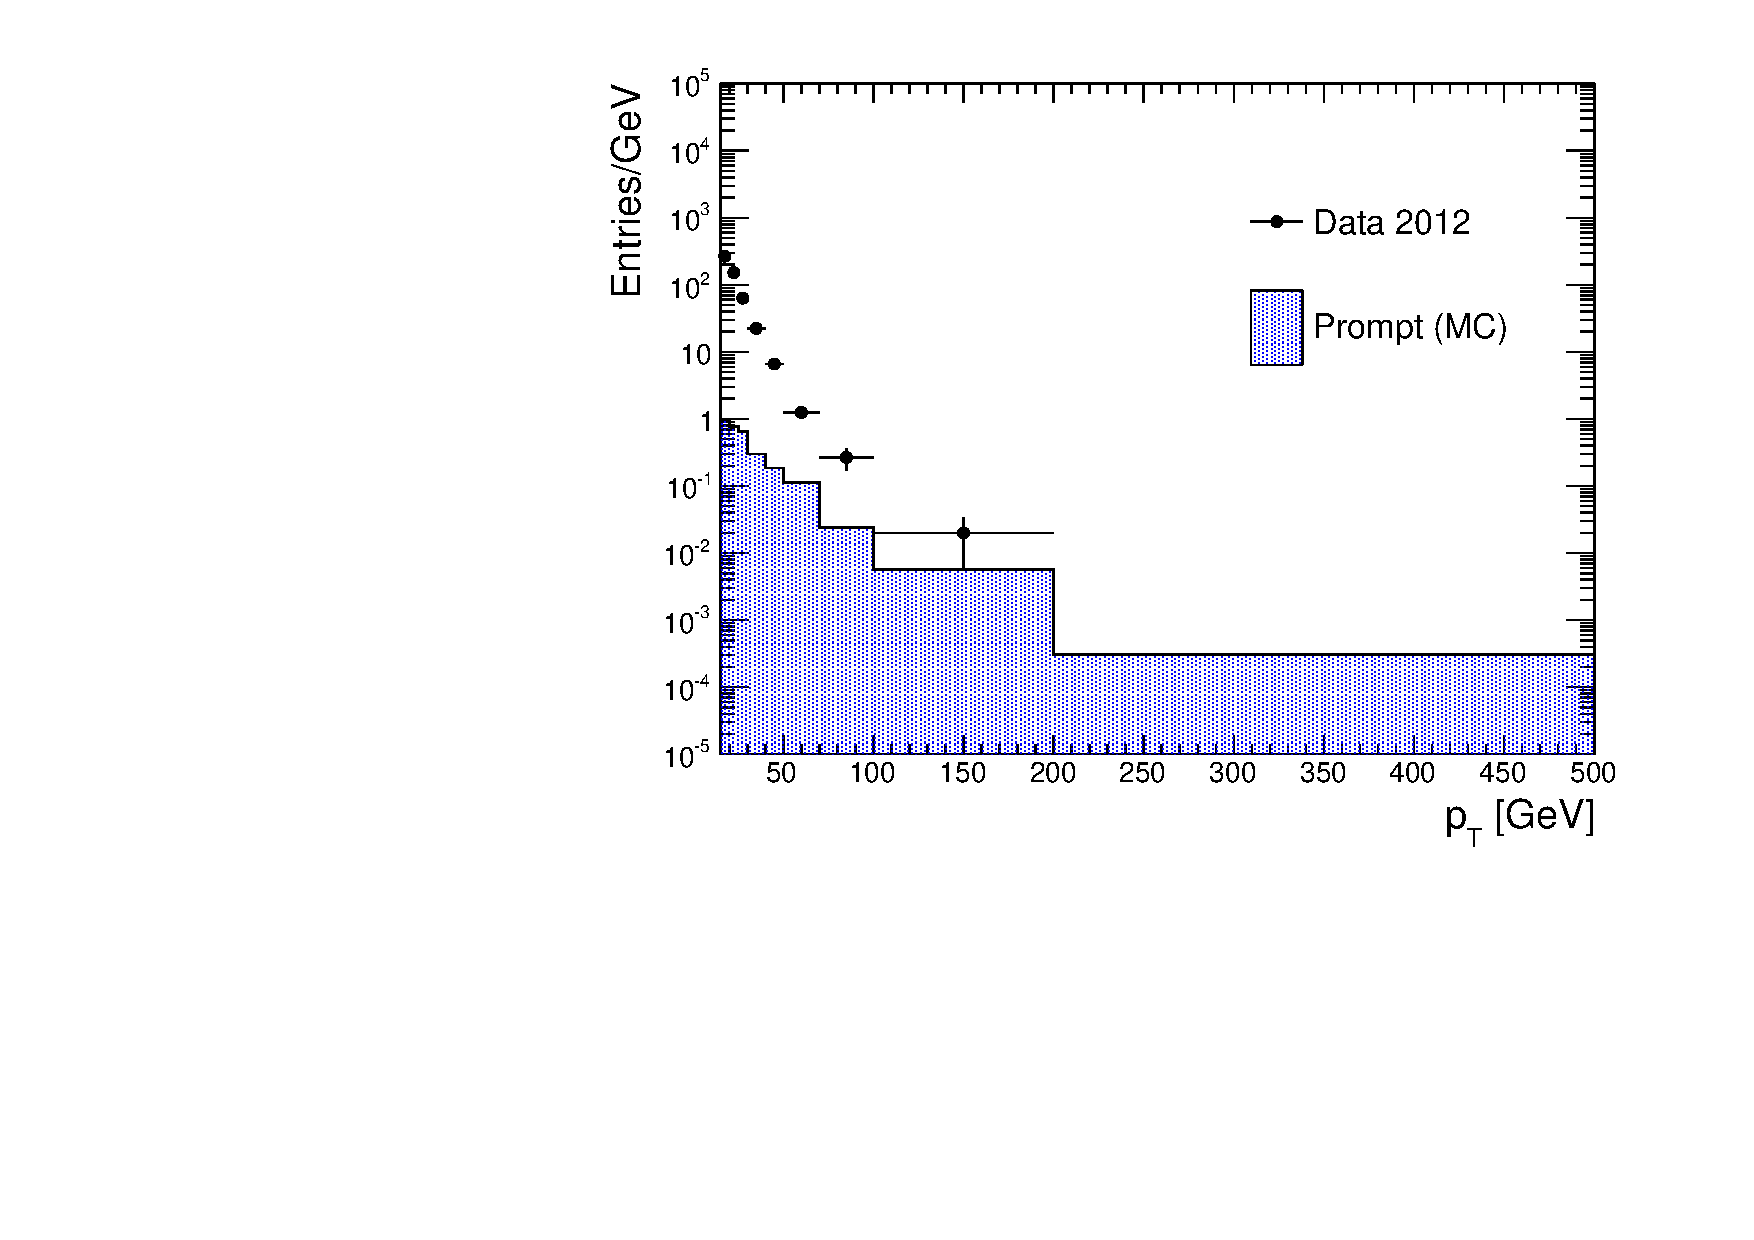
\includegraphics[width=0.3\columnwidth]{figures/ch5-model-independent/num__1jet__sldr}
  }
  \subfloat[Numerators, 2-jet]{
	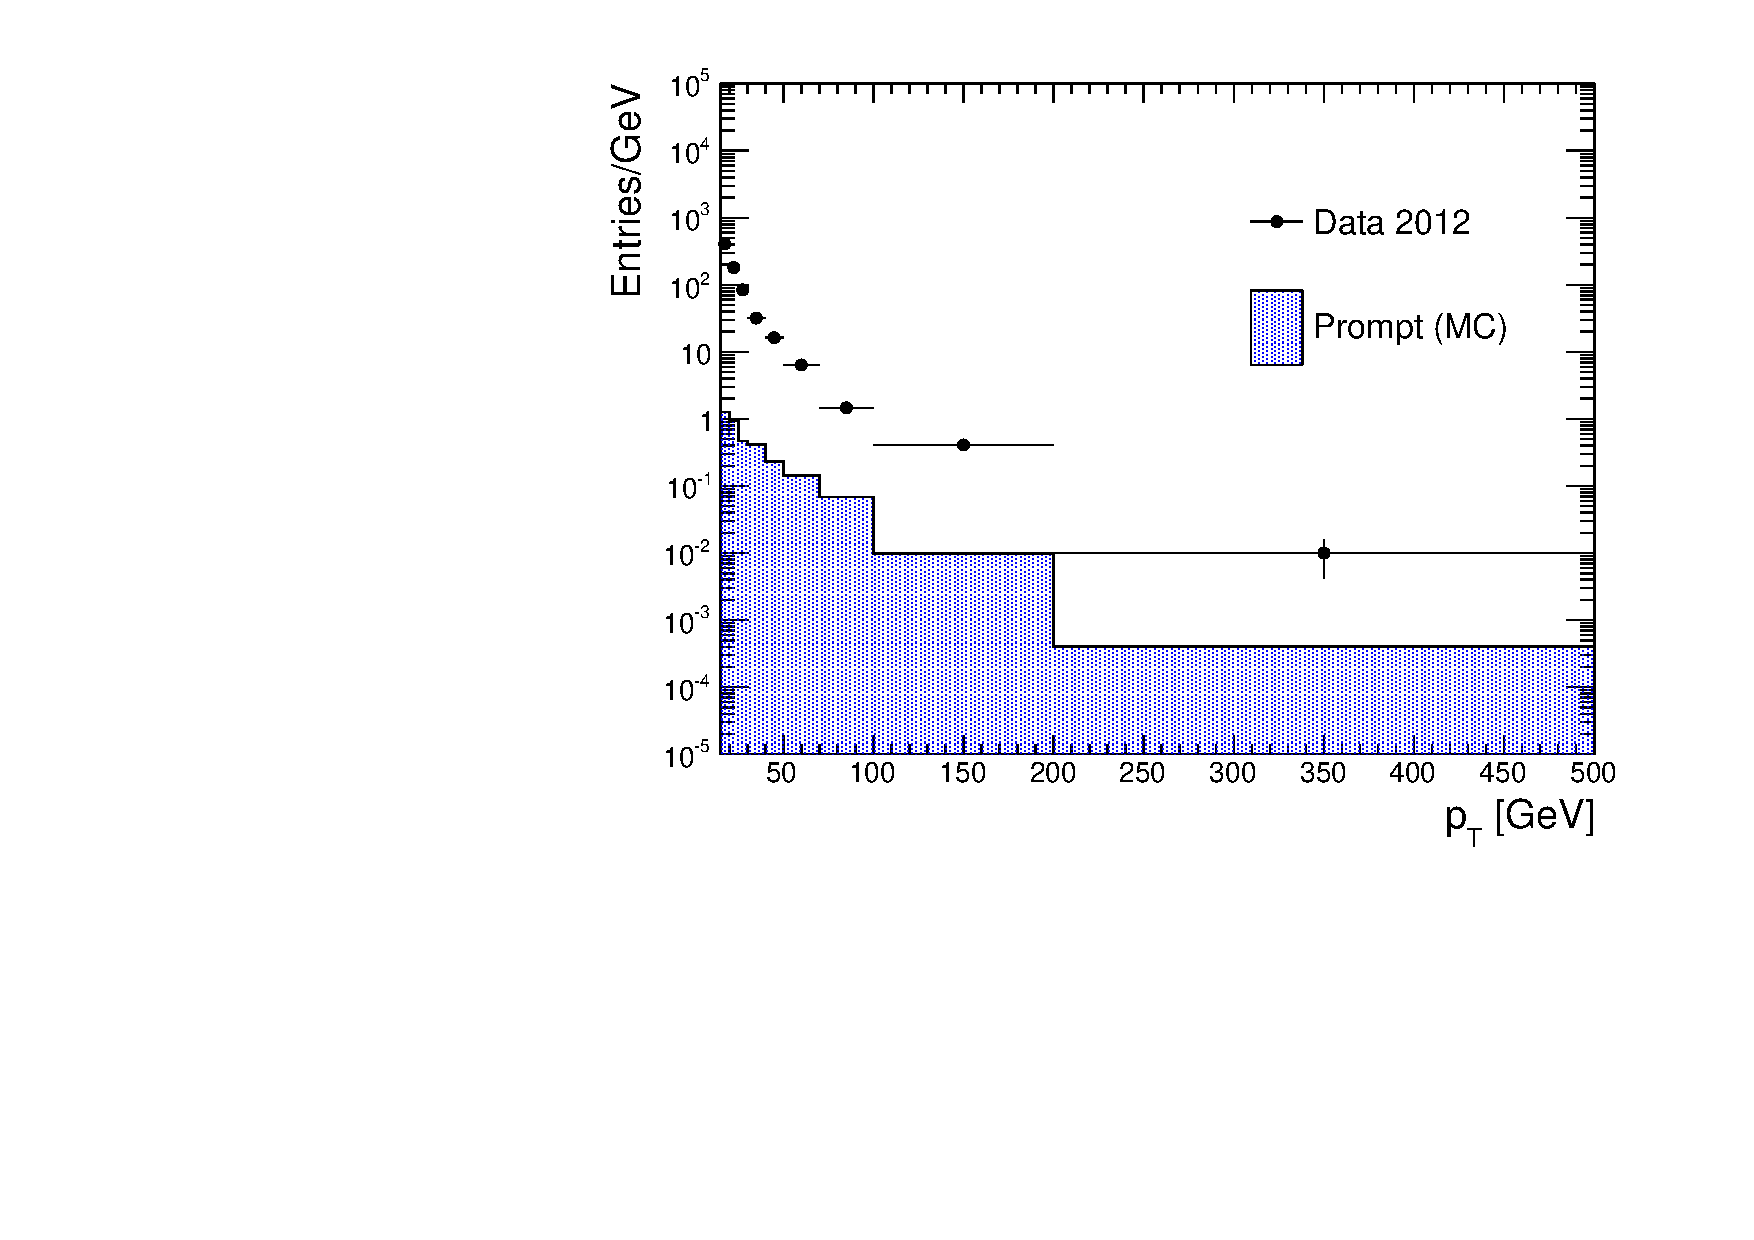
\includegraphics[width=0.3\columnwidth]{figures/ch5-model-independent/num__2jet__sldr}
  }\\
  \subfloat[Denominators, 0-jet]{
	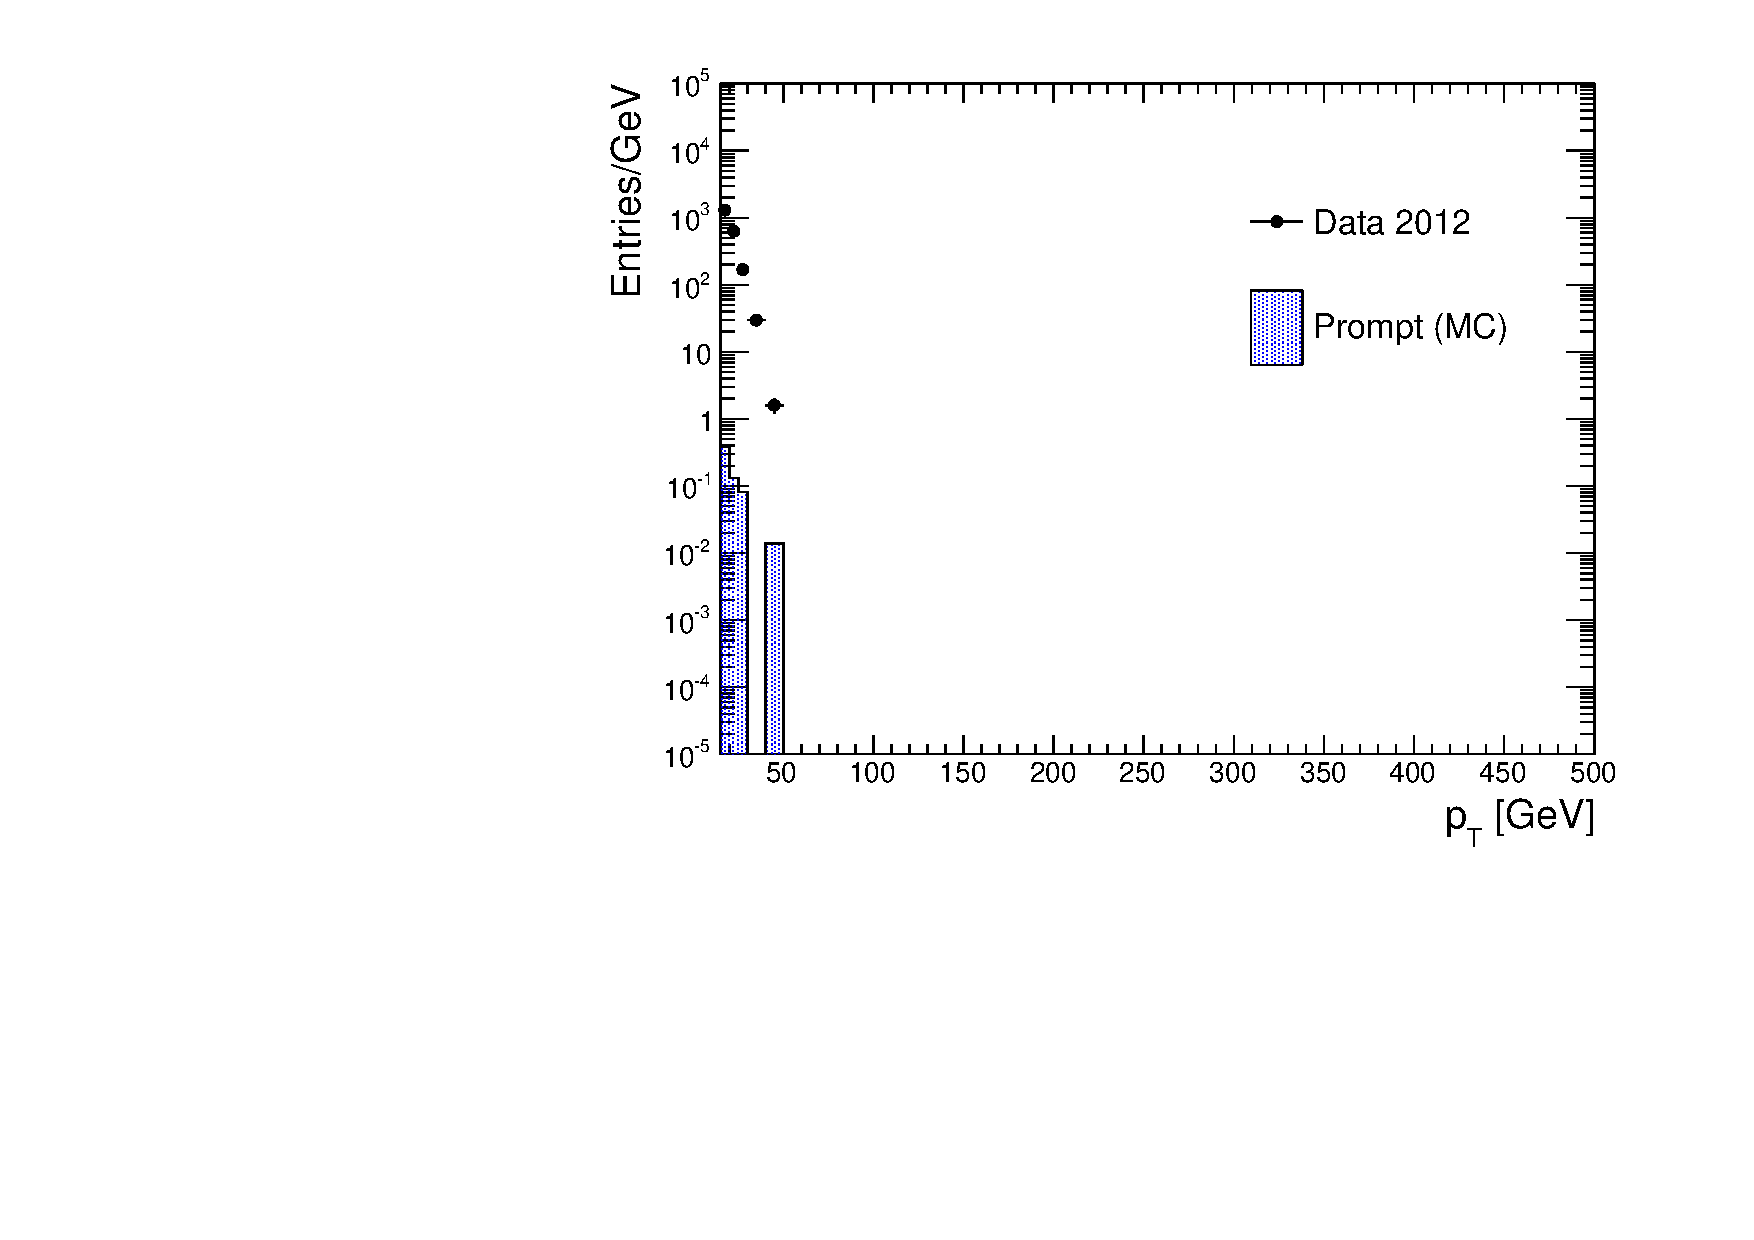
\includegraphics[width=0.3\columnwidth]{figures/ch5-model-independent/den__0jet__nodr}
  }
  \subfloat[Denominators, 1-jet]{
	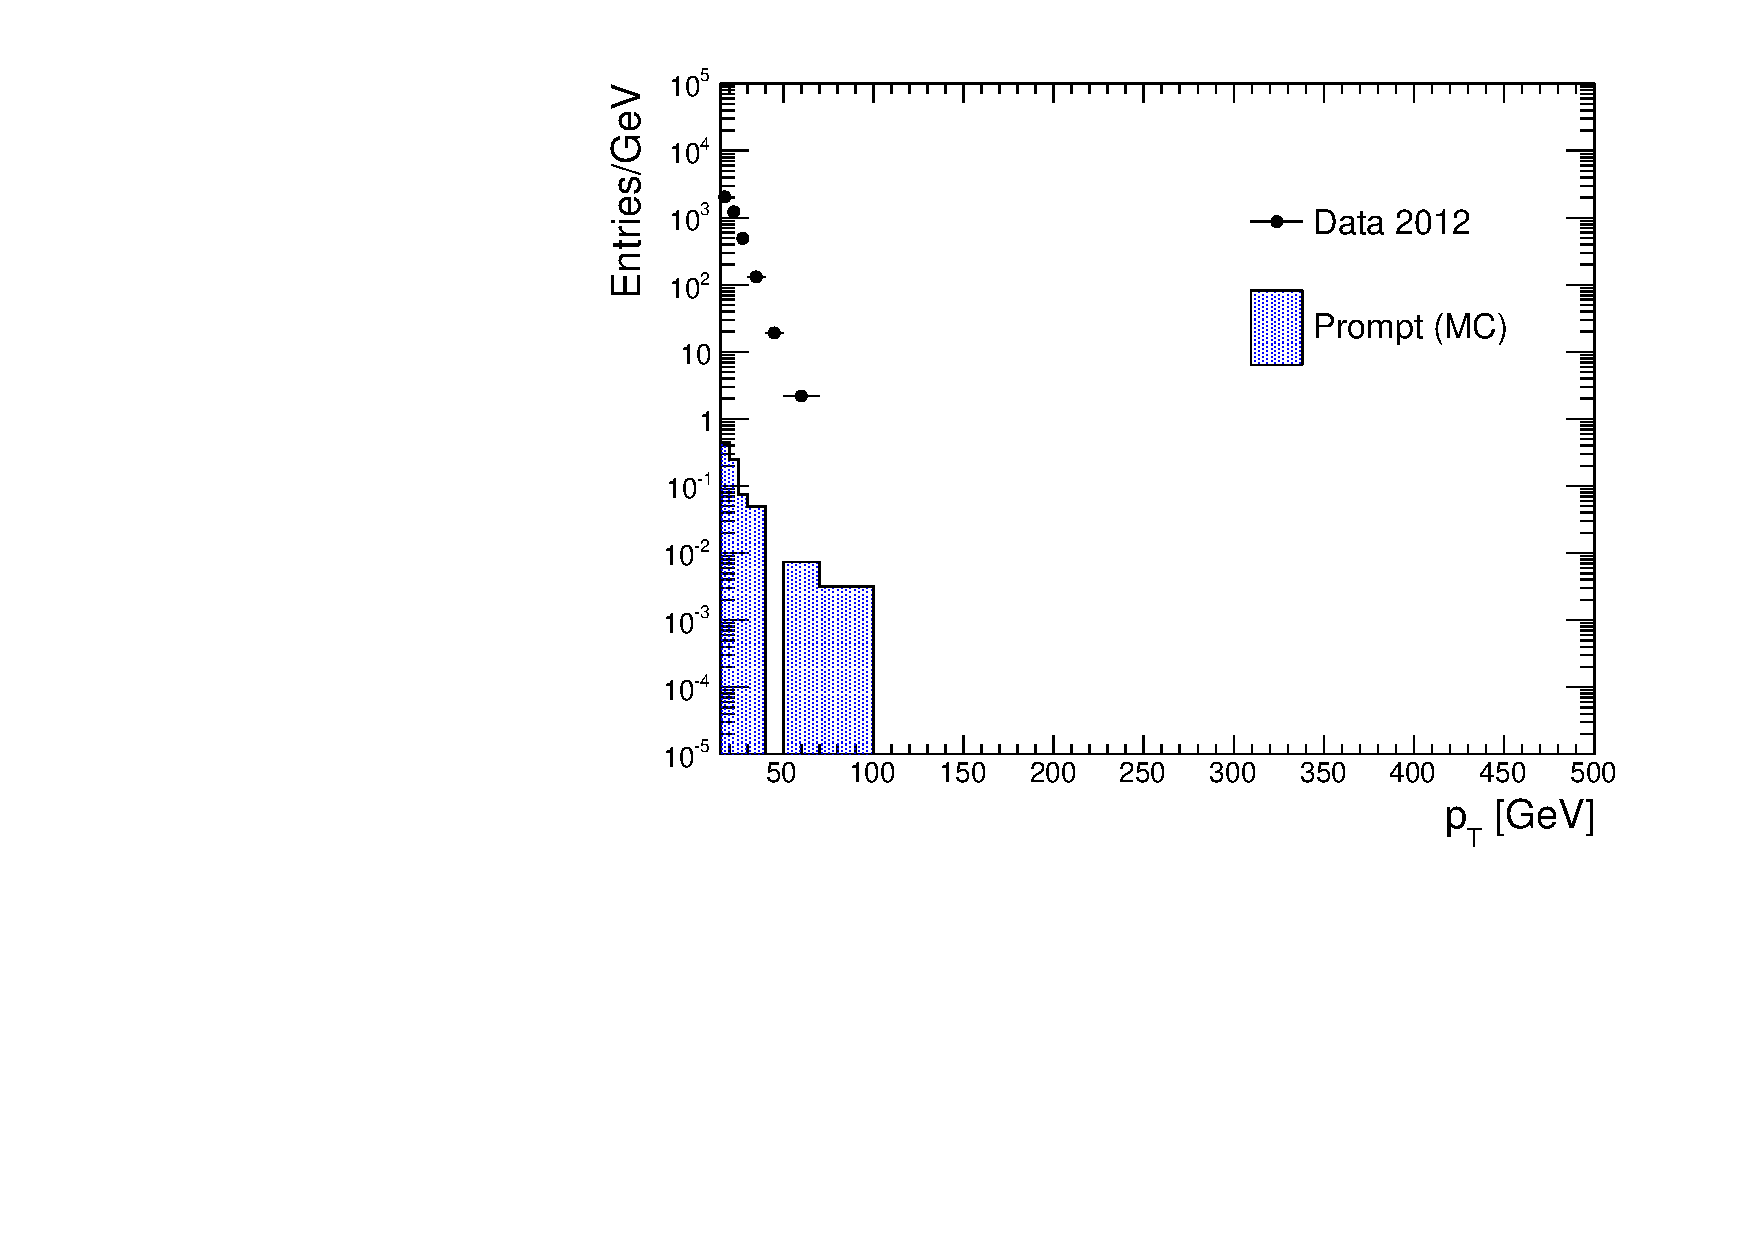
\includegraphics[width=0.3\columnwidth]{figures/ch5-model-independent/den__1jet__sldr}
  }
  \subfloat[Denoninators, 2-jet]{
	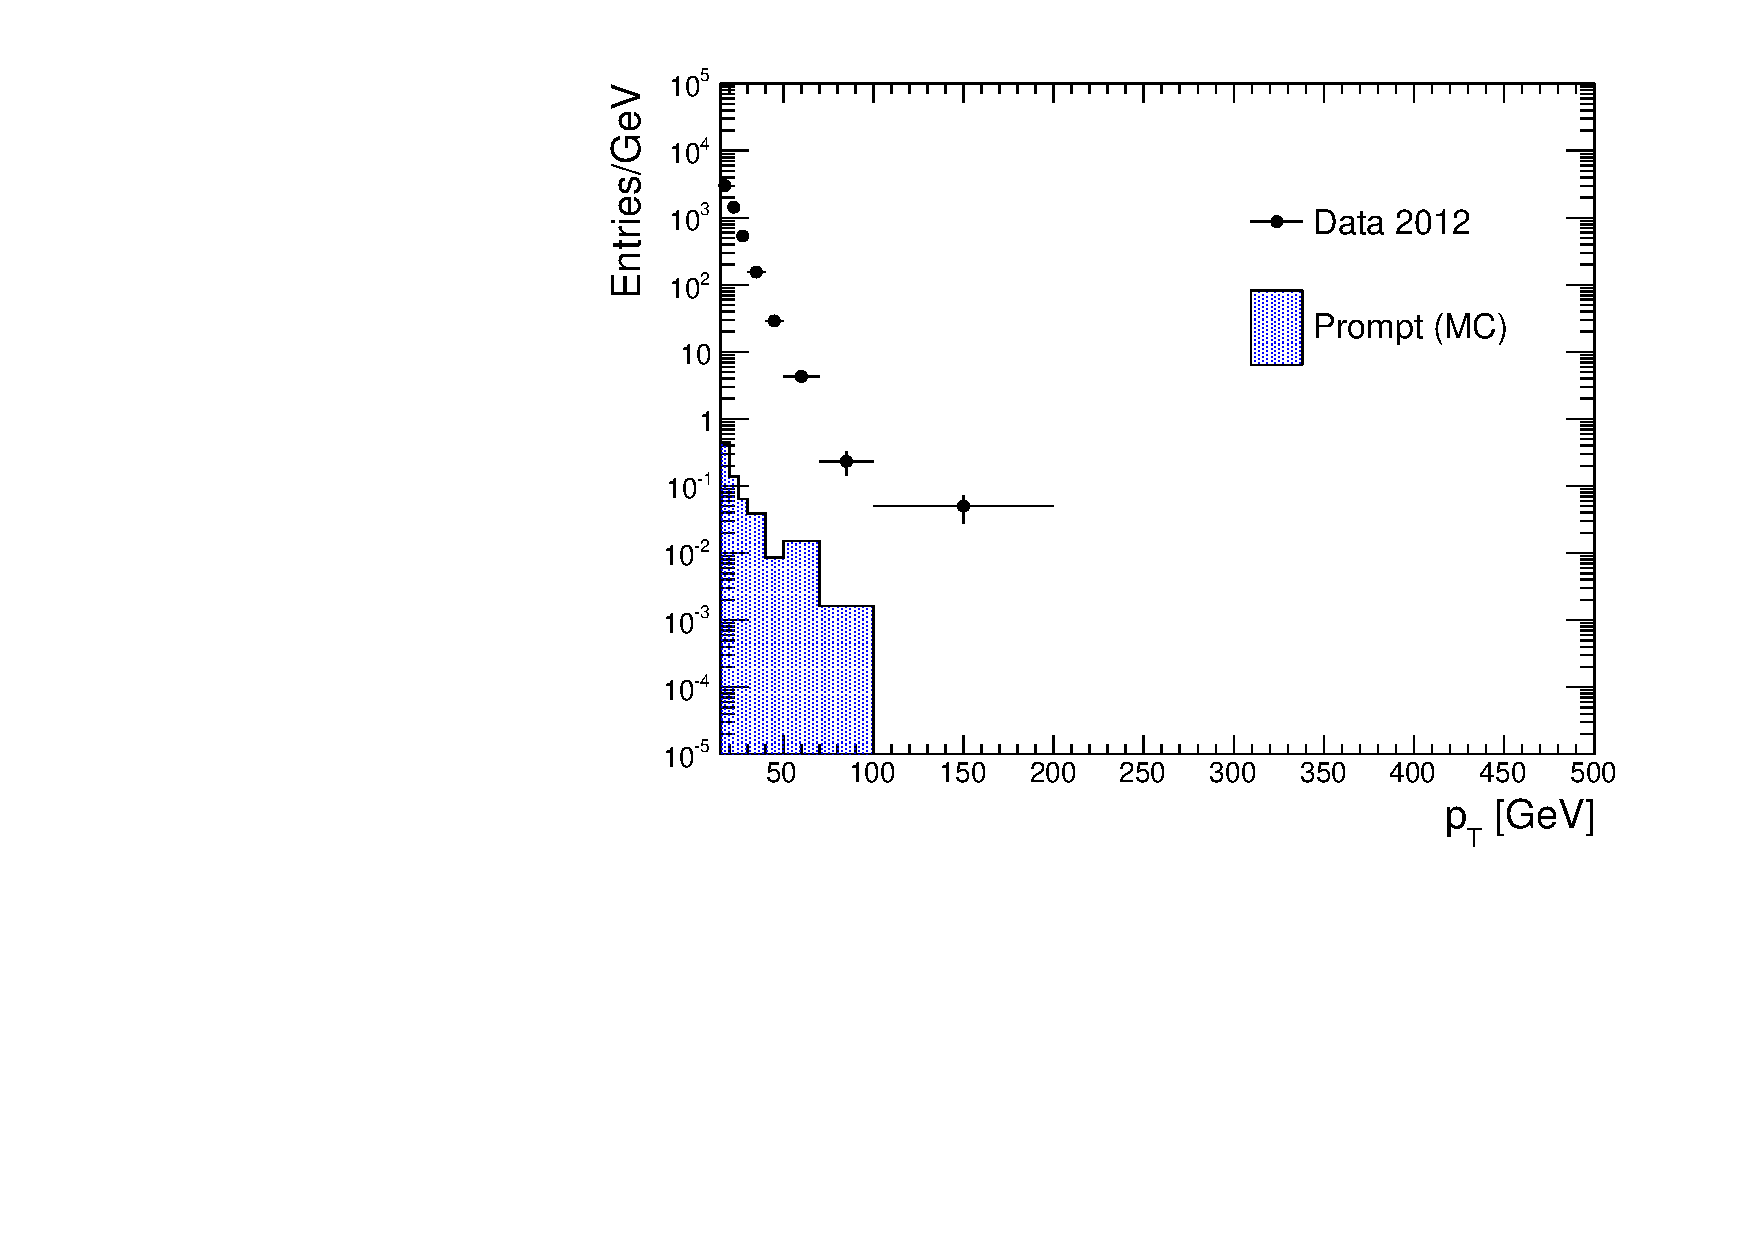
\includegraphics[width=0.3\columnwidth]{figures/ch5-model-independent/den__2jet__sldr}
  }\\
  \subfloat[Denominators, 0-jet]{
	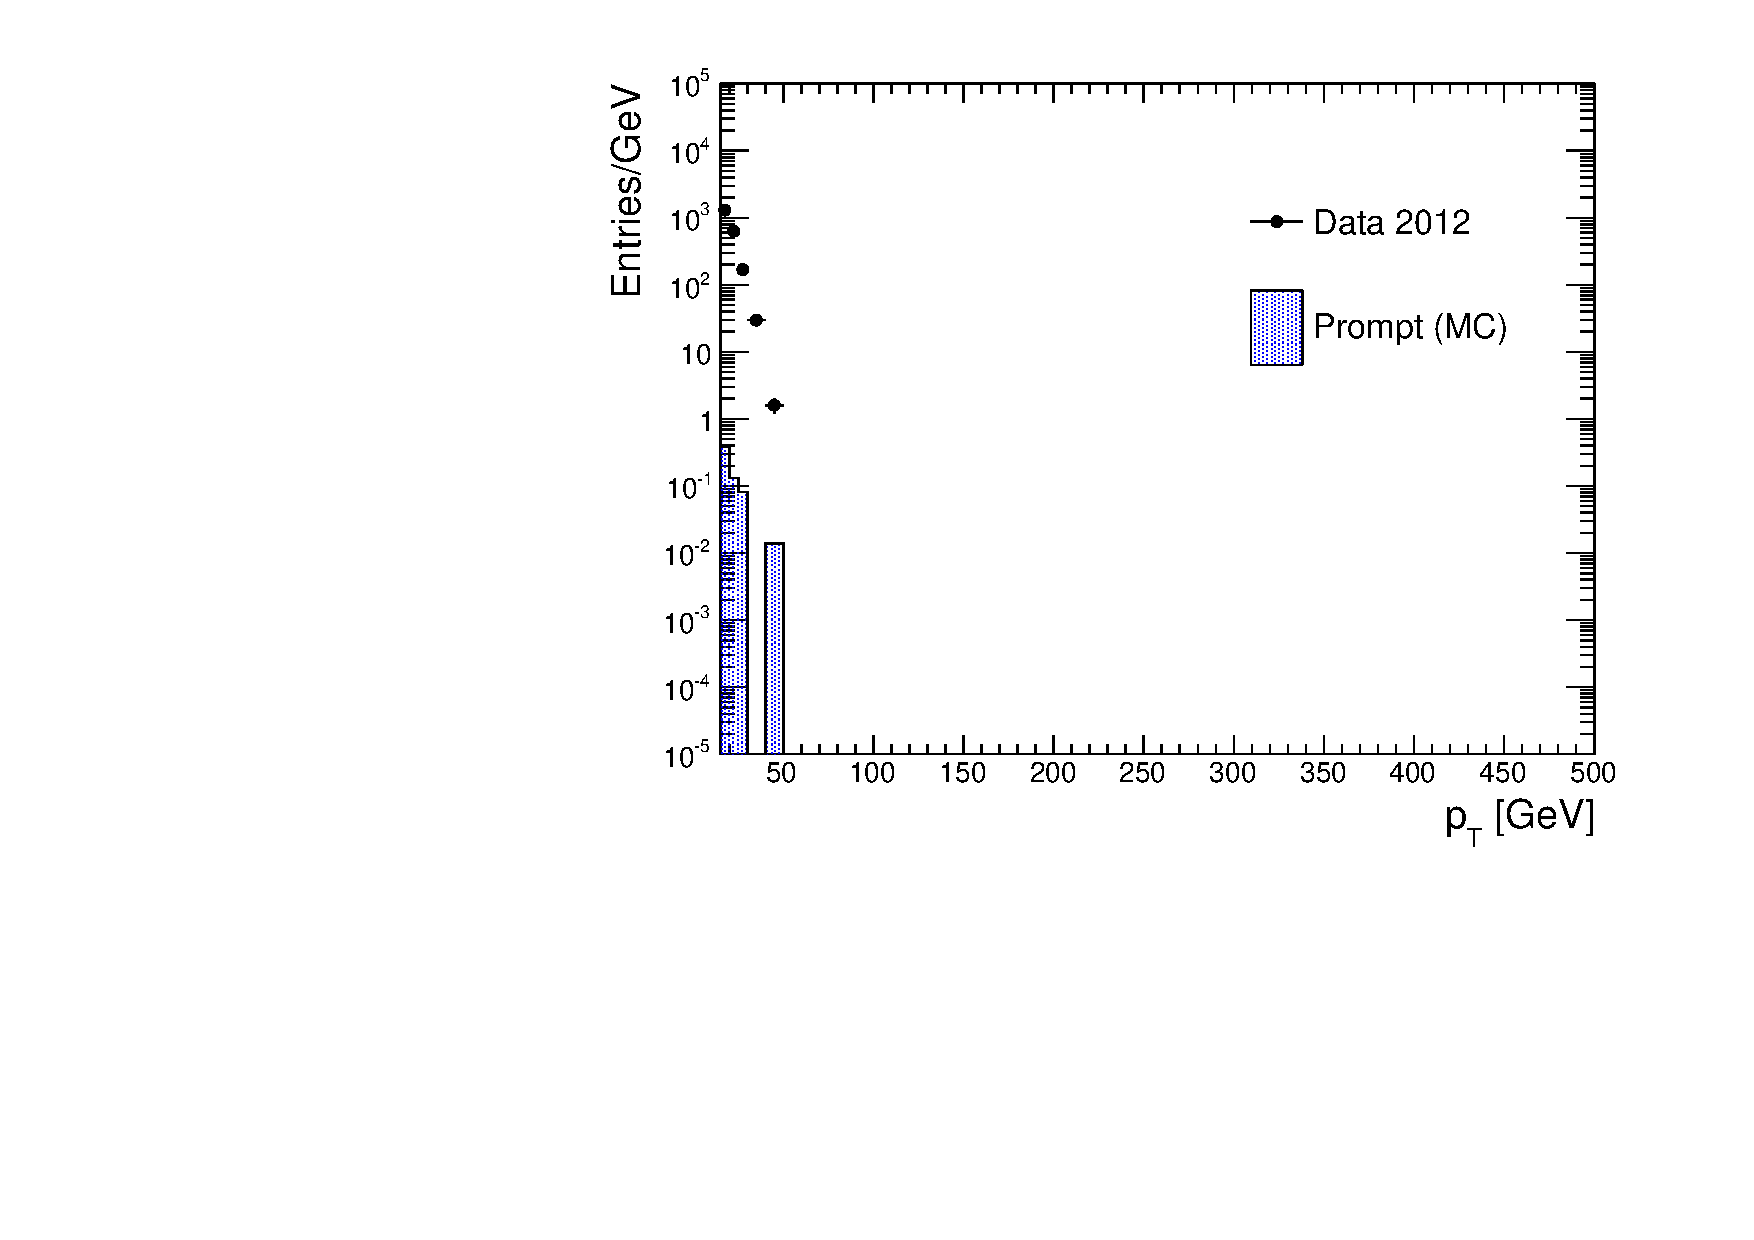
\includegraphics[width=0.3\columnwidth]{figures/ch5-model-independent/den__0jet__nodr}
  }
  \subfloat[Denominators, 1-jet]{
	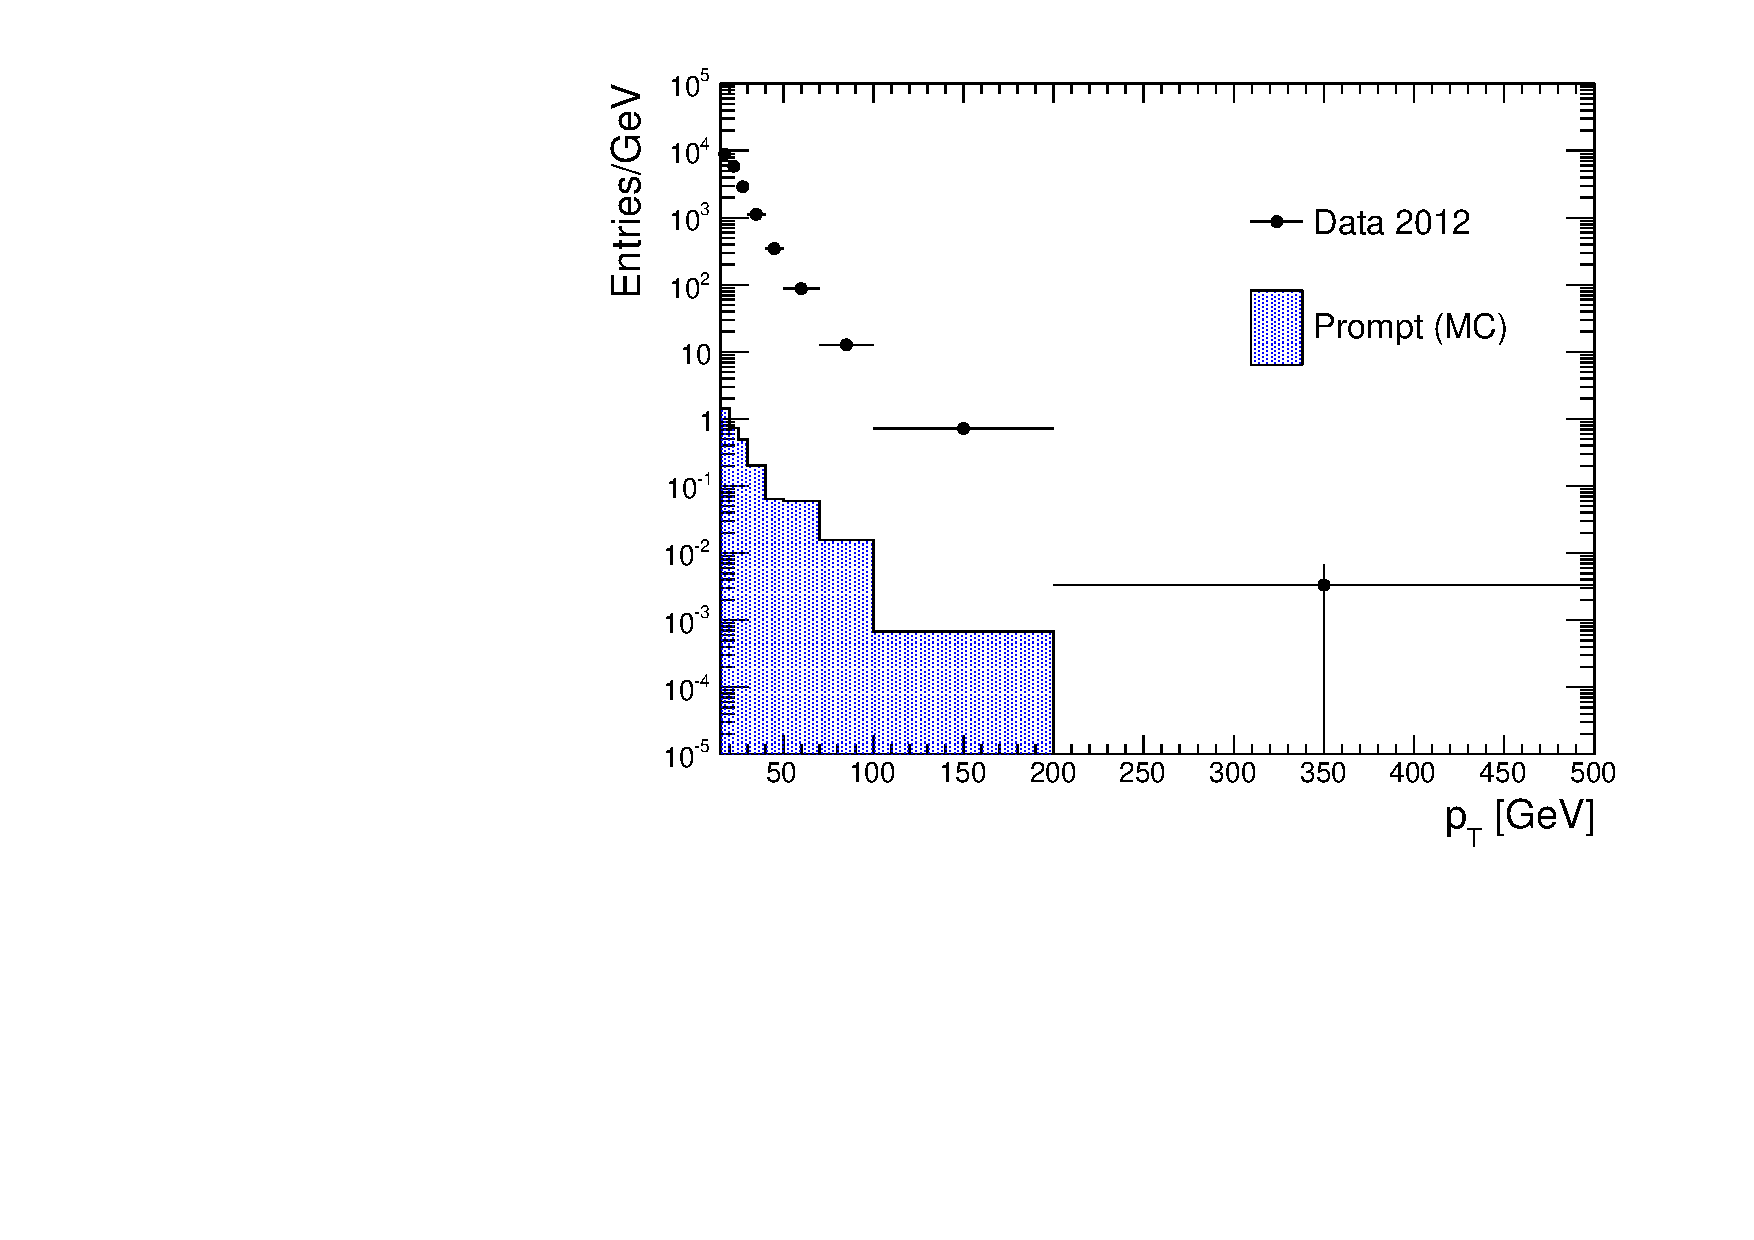
\includegraphics[width=0.3\columnwidth]{figures/ch5-model-independent/den__1jet__nodr}
  }
  \subfloat[Denominators, 2-jet]{
	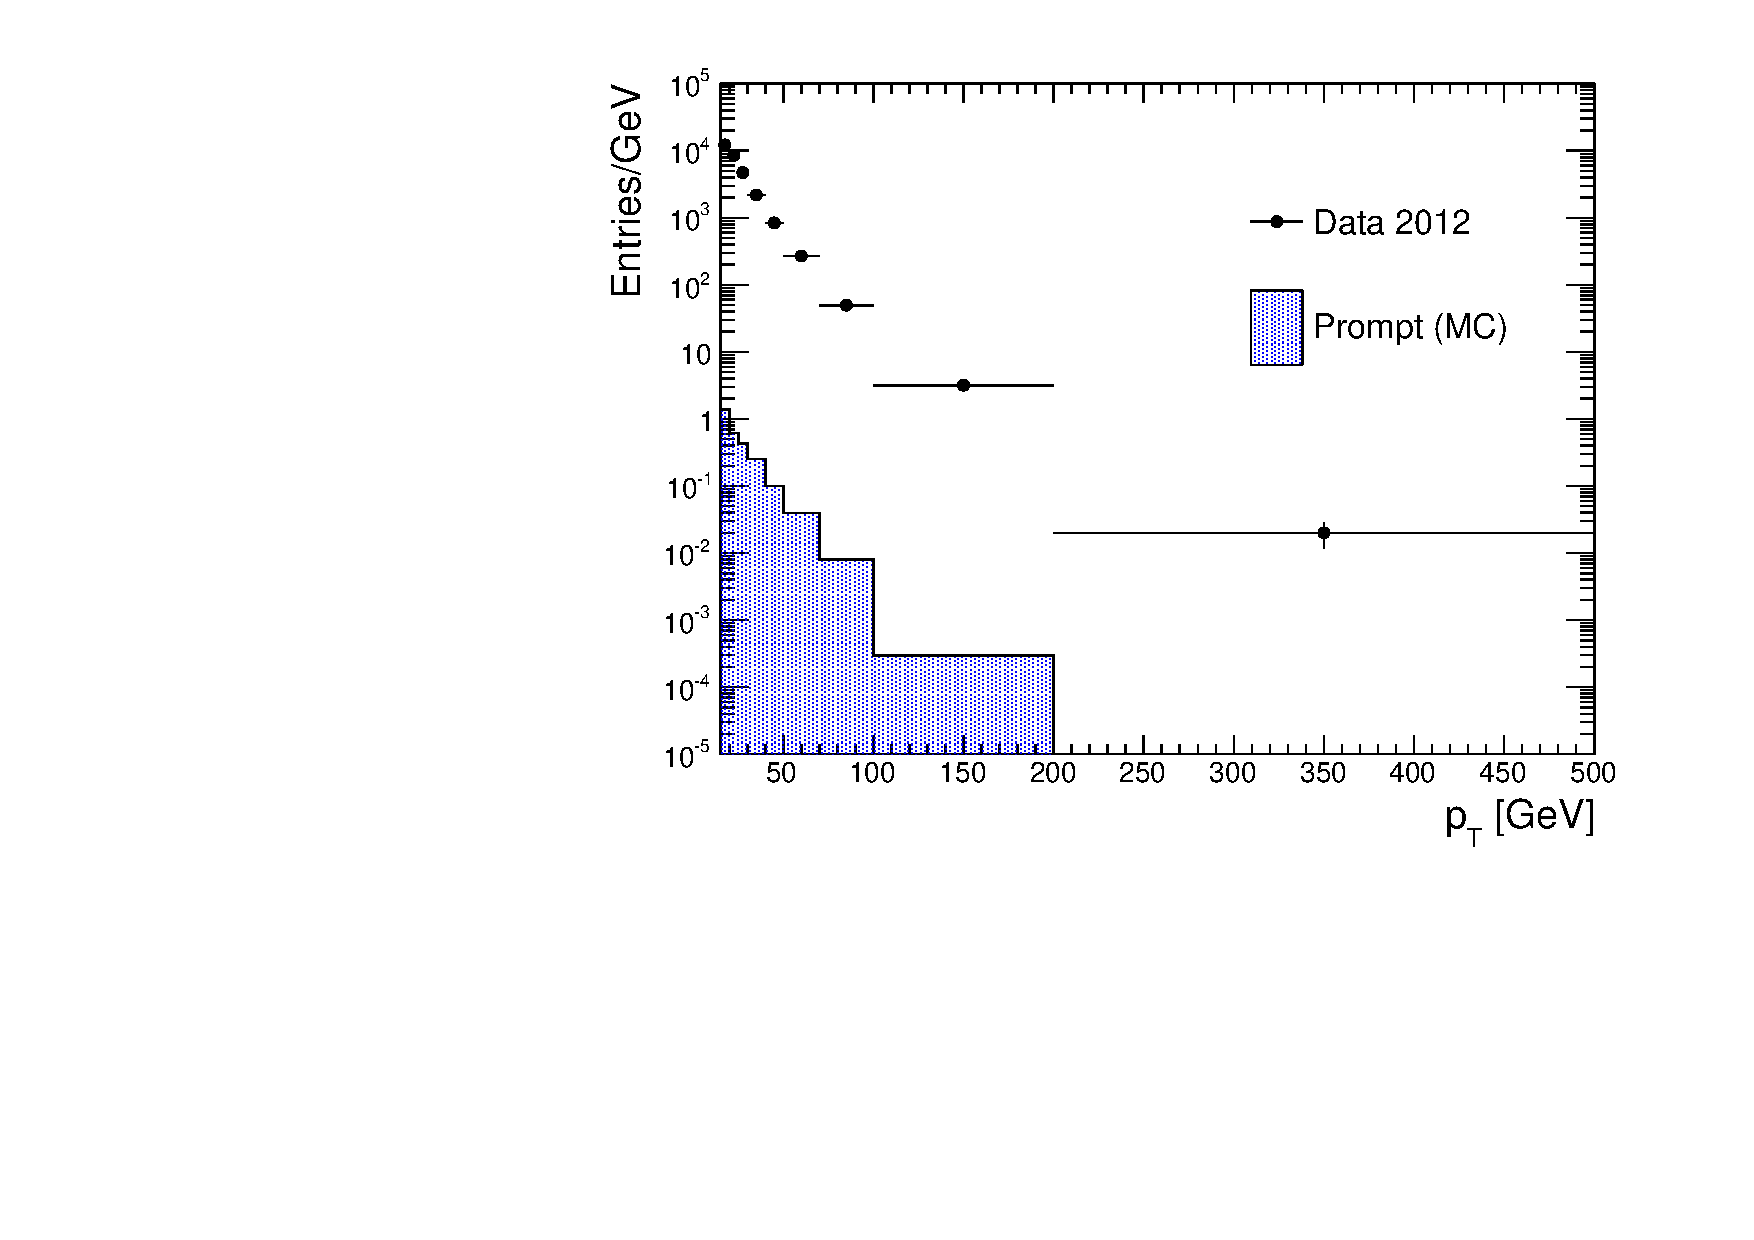
\includegraphics[width=0.3\columnwidth]{figures/ch5-model-independent/den__2jet__nodr}
  }

  \caption{\label{fig:MuFake_stacks}$\pt$ spectrum of muons used in fake factor measurement.  The left plots show events with zero jets, the middle
	plots show events with one jet, and the right plots show events with two or more jets.  All numerator events require both numerator and denominator be separated from a jet by $\Delta R > 0.3$; the same requirement is applied to denominators in the second row of plots, while the third row shows 
denominators that are not required to be isolated from nearby jets.}
\end{figure}


The extrapolation factor from the measurement control region, with $|\frac{d_0}{\sigma_{d_0}}|>3$, to the signal region, with $|\frac{d_0}{\sigma_{d_0}}|<3$, is derived from various Monte Carlo samples. The extrapolation factor is simply the ratio of fake factors derived in Monte Carlo using the control region cut ($|\frac{d_0}{\sigma_{d_0}}|>3$) to those using the signal region cut ($|\frac{d_0}{\sigma_{d_0}}|<3$). The central value is taken from the \powheg~$t\overline{t}$ sample, using all truth-level non-prompt muons, as shown in figure~\ref{fig:MuFake_extrap}. A systematic uncertainty is assigned by comparing with other samples (\mcatnlo $t\overline{t}$ and \pythiab $b\overline{b}$ and $c\overline{c}$), and using only same-sign dimuon events in these samples.  

\begin{figure}[h]
\centering 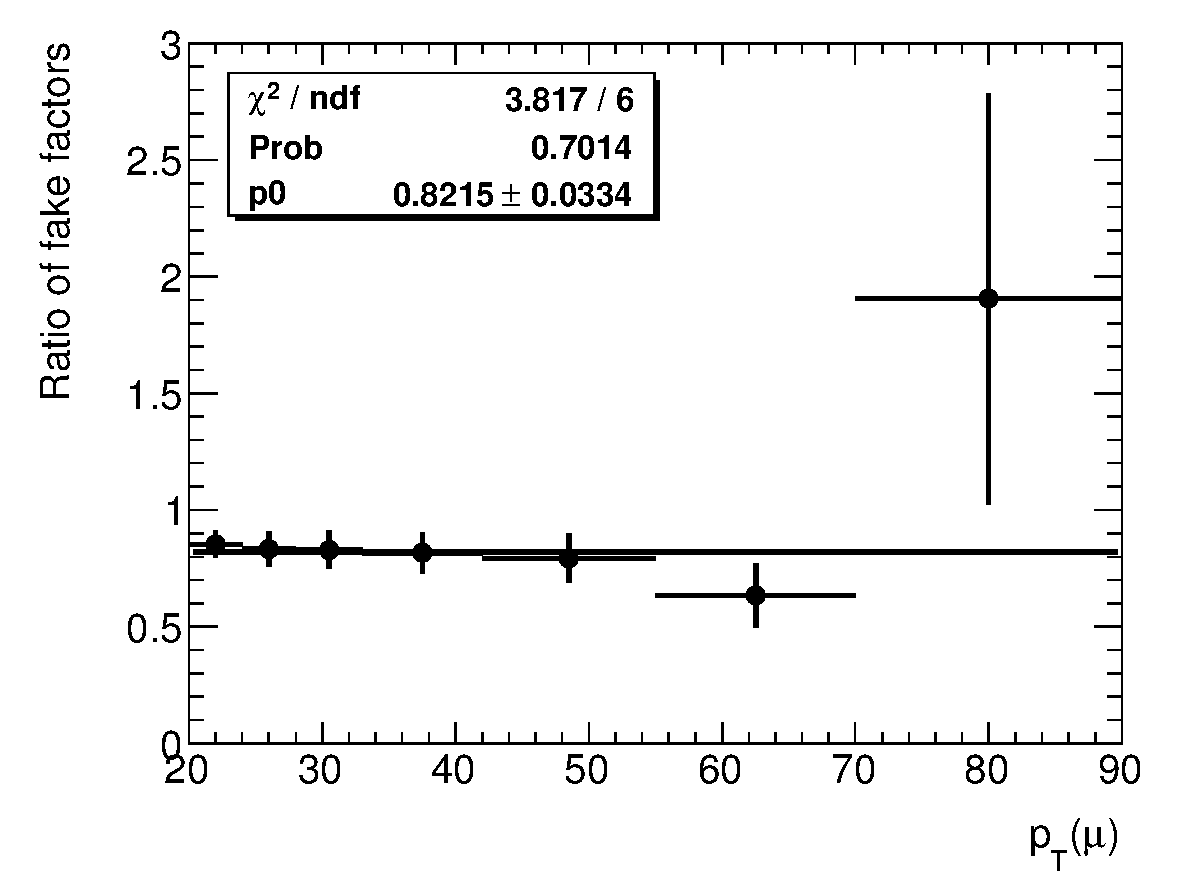
\includegraphics[width=0.48\textwidth]{figures/ch5-model-independent/MuFake_extrap_ratio}
\caption{\label{fig:MuFake_extrap}Ratio between the fake factors for muons with $|d_0|/\sigma(d_0)>3$ compared to fake factor with nominal numerator and denominator 
definitions.  These fake factors are derived from a \powheg $t\bar{t}$ sample.}
\end{figure}

The fake factors are parametrized one-dimensionally in $\pt$ and $\eta$, as there are insufficient statistics to do a full two-dimensional parametrization. The fake factor is computed as:
\begin{equation}
f(\pt,\ \eta) = \frac{f(\pt)\times f(\eta)}{\langle f \rangle}
\end{equation}
where $\langle f \rangle$ is the total average fake factor. The measured fake factors are shown in figures~\ref{fig:MuFake_ff_1D} and \ref{fig:MuFake_ff}. 

\begin{figure}
\centering 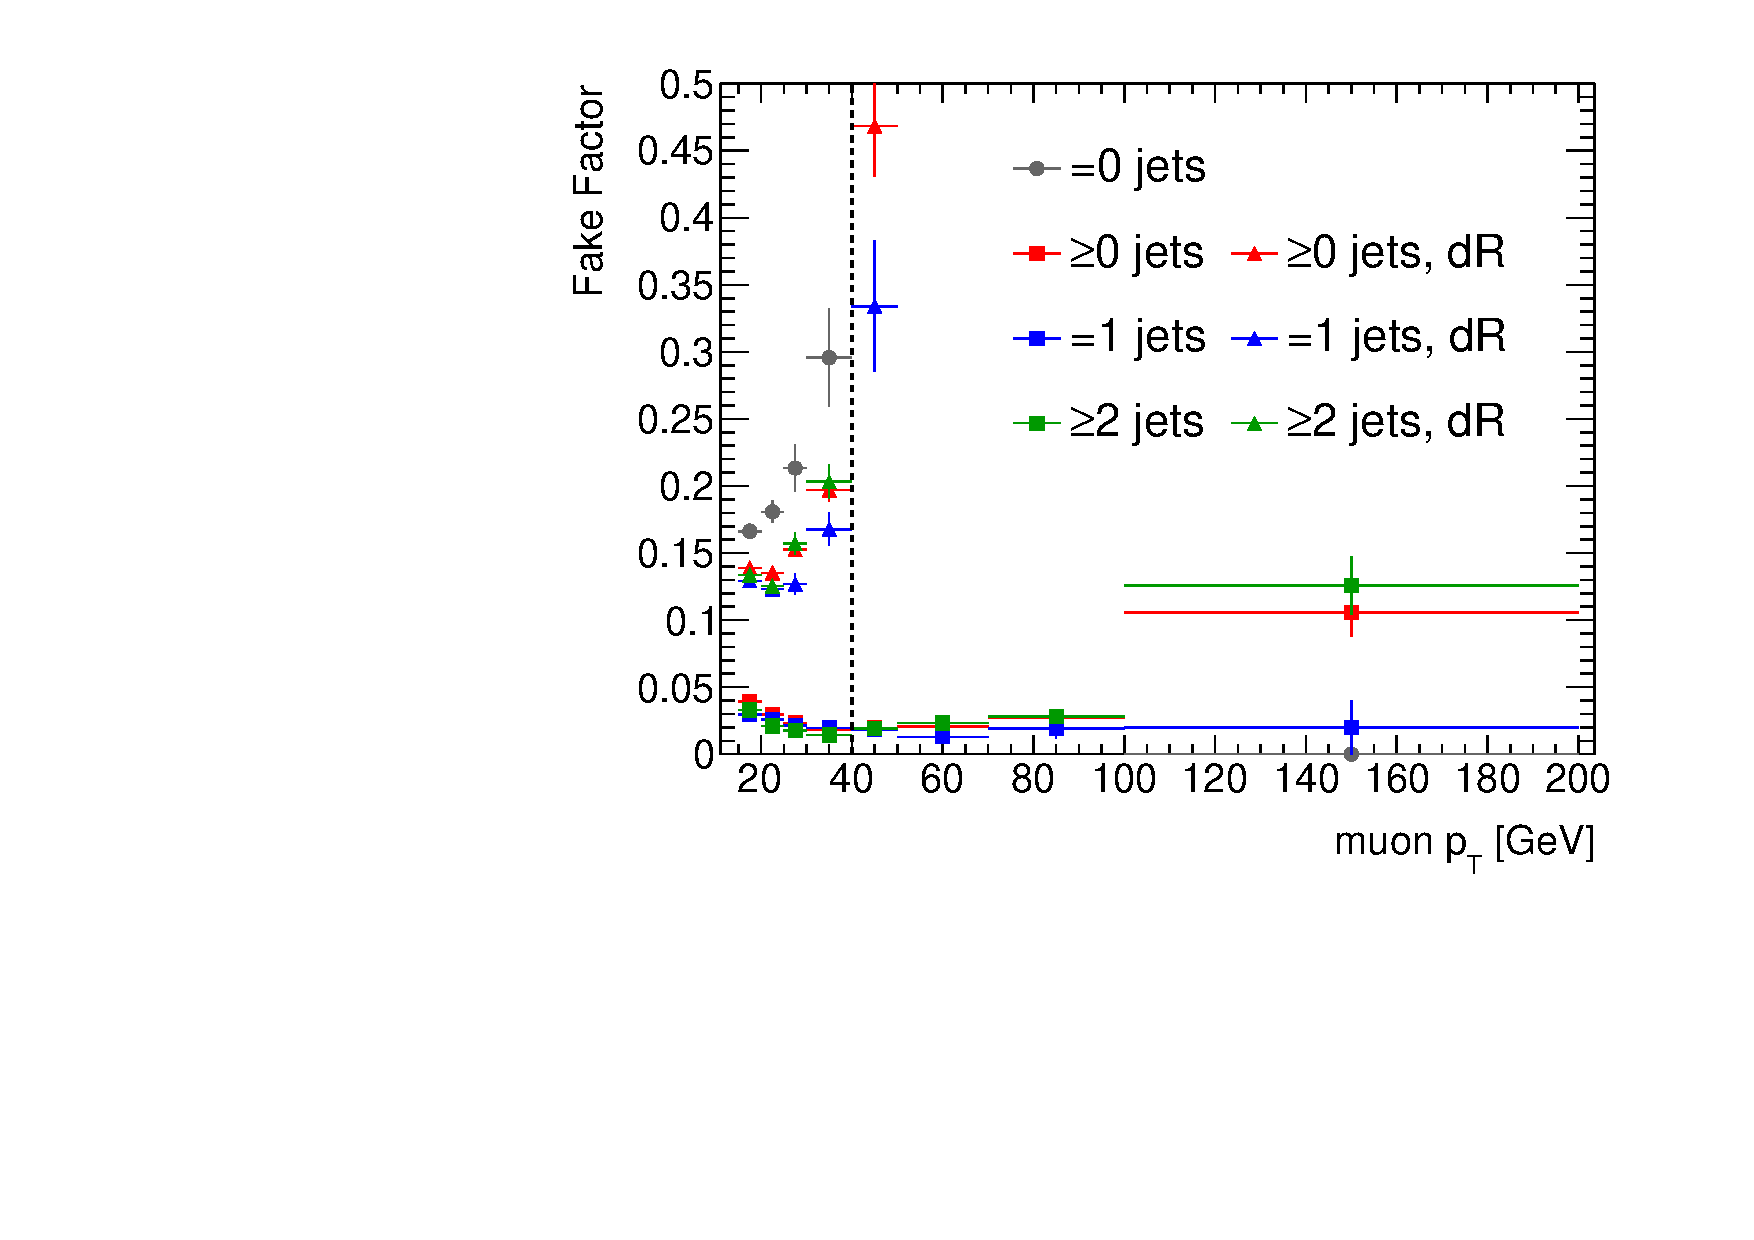
\includegraphics[width=0.48\textwidth]{figures/ch5-model-independent/all_1D_pt}
%\centering \includegraphics[width=0.48\textwidth]{figures/ch5-model-independent/MuFake_ff_vseta}
\caption{\label{fig:MuFake_ff_1D}Muon fake factors as a function of $\pt$. Two sets of fake factors are plotted, with and without the ``dR'' requirement. The vertical dashed line at 40 GeV indicates the point at which the fake factors switch from the ``dR'' points, where the denominators are required to be separated from nearby jets, to the lower, non-''dR'' points where the jet-isolation requirement is dropped to improve the statistics.}
\end{figure}

\begin{figure}
  \subfloat[Inclusive FF] {
	\resizebox{0.48\textwidth}{!}{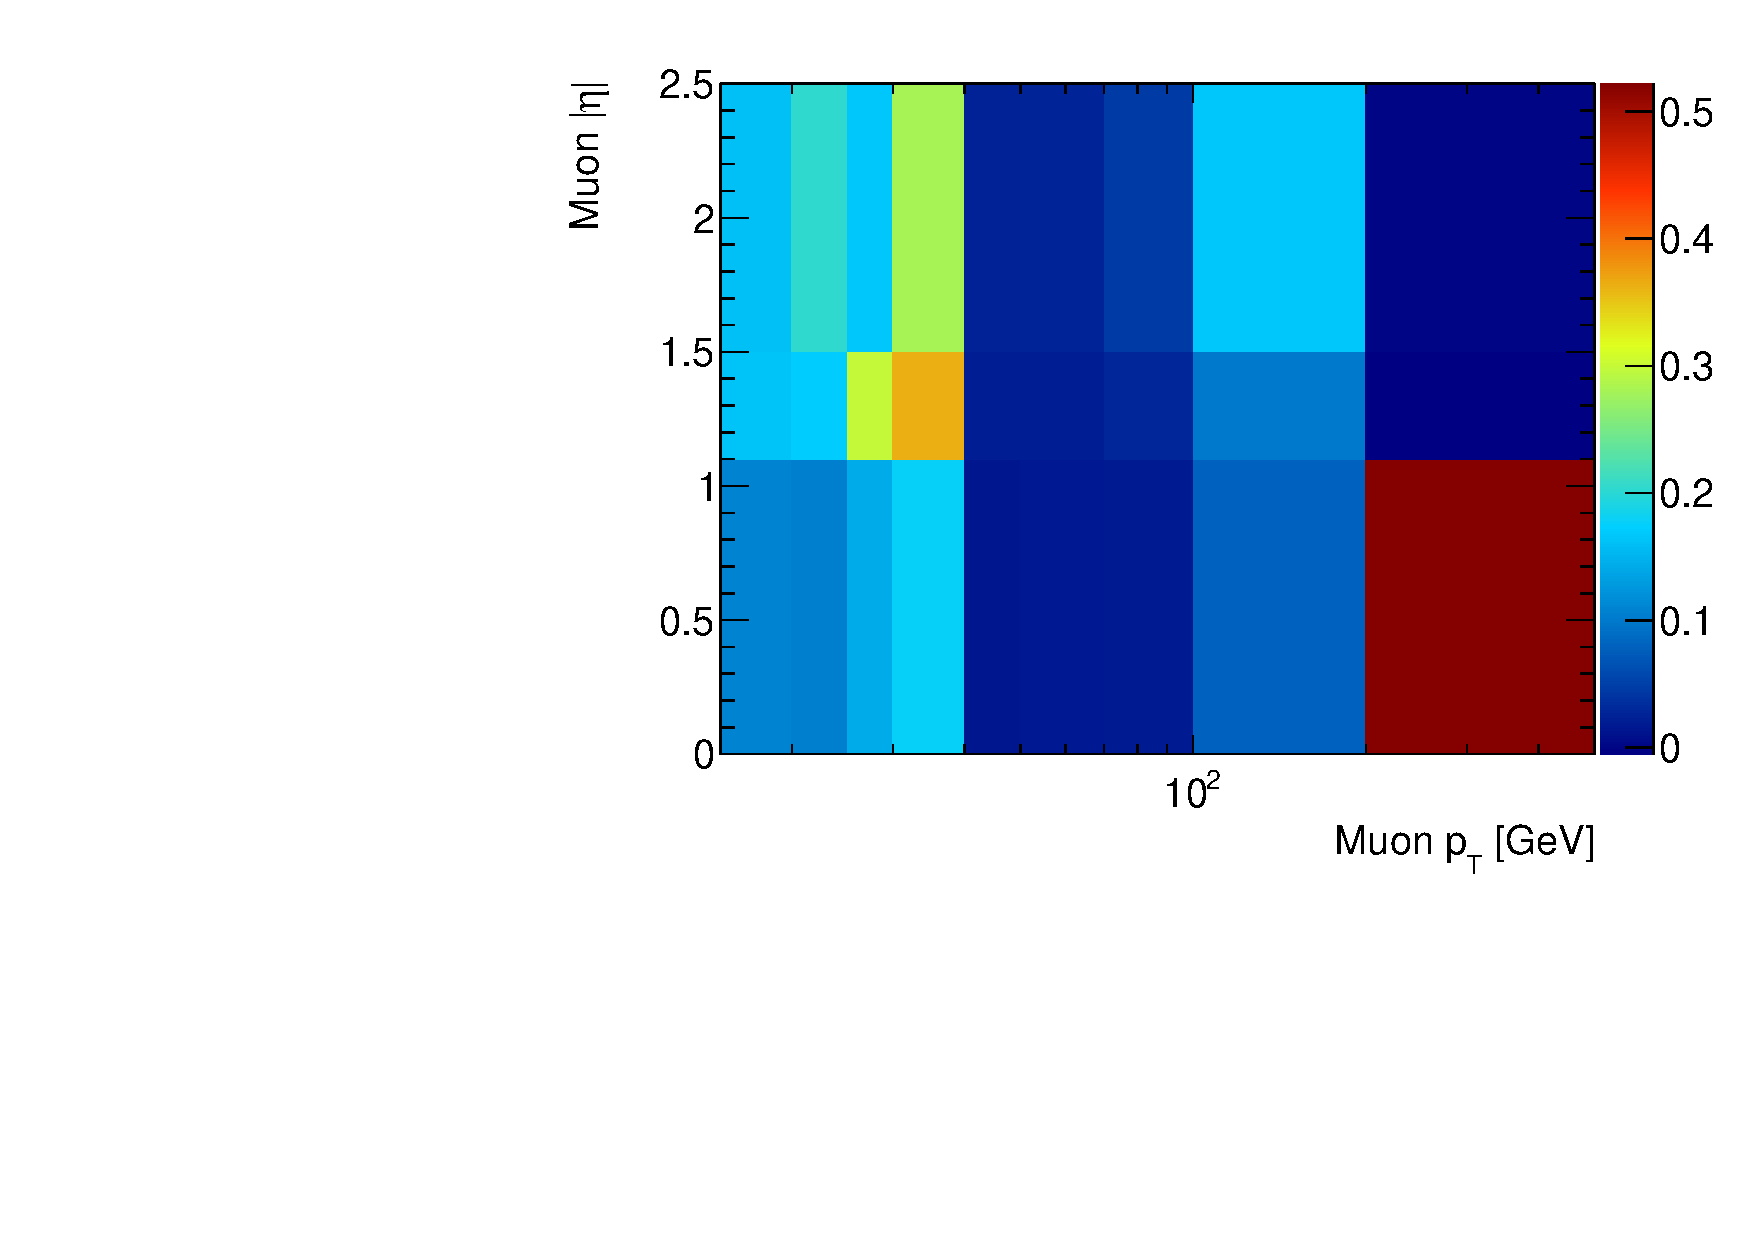
\includegraphics{figures/ch5-model-independent/ff_0jet_final}}
  }
  \subfloat[Two-jet FF] {
	\resizebox{0.48\textwidth}{!}{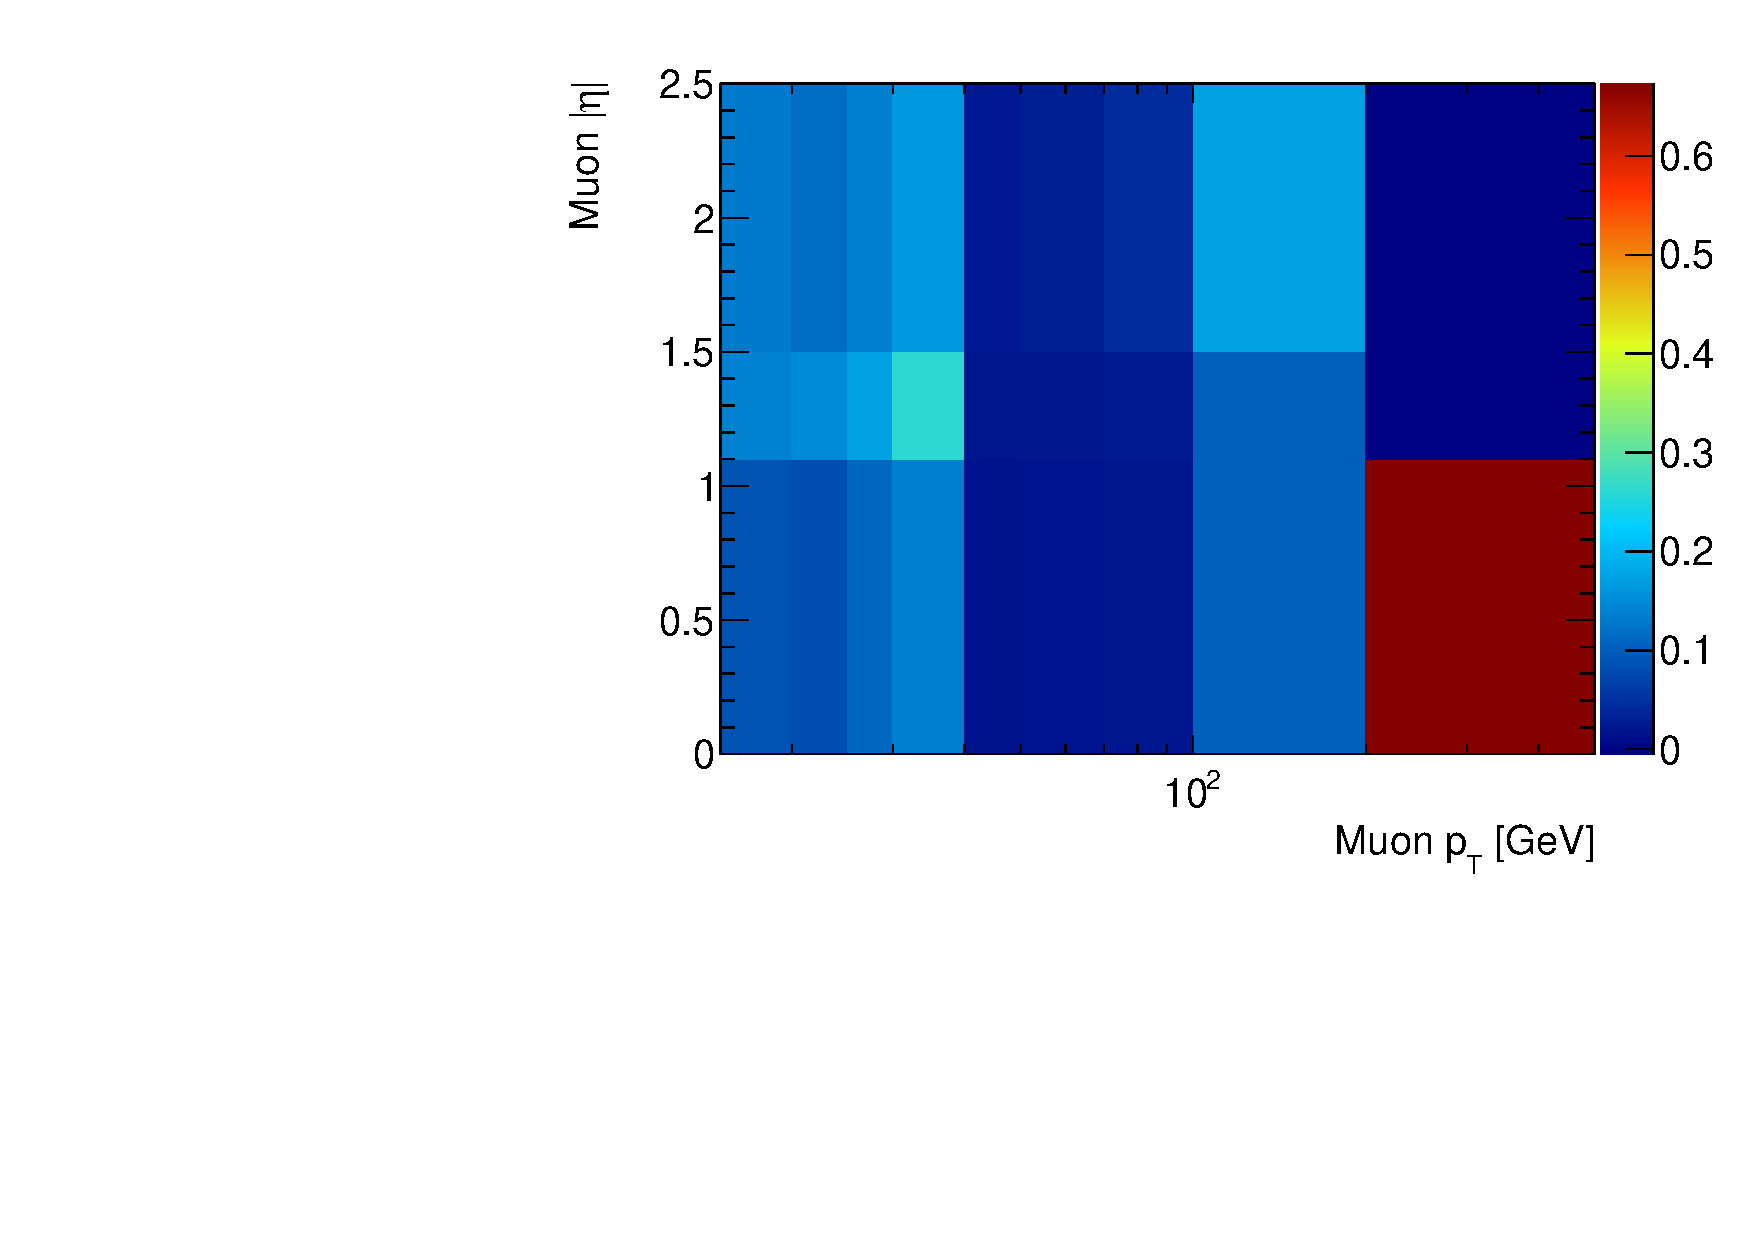
\includegraphics{figures/ch5-model-independent/ff_2jet_final}}
  }
  \caption{Muon fake factors as functions of $\pt$ and $|\eta|$.  The left plot shows fake factors measured in the inclusive control sample and applied to events with zero jets. The right plot shows fake factors measured in events with two jets, and applied to events with at least one jet.}
  \label{fig:MuFake_ff}
\end{figure}


The sources of systematic uncertainty considered are listed below, and the fractional systematic uncertainty is shown in figure~\ref{fig:MuFake_syst}.

\begin{itemize}
  \item \textbf{Prompt subtraction}: The normalization of the simulated prompt subtraction samples is varied by $\pm10\%$, leading to a systematic uncertainty of $1$-$6\%$.
  \item \textbf{Topological dependence}: The difference between the inclusive and two-jet fake factors is taken as a systematic uncertainty. The uncertainty is symmetrized, using the full difference as both upward and downward uncertainty, and ranges from $3\%$ to $36\%$. 
  \item \textbf{Dependence on $d_0$ significance}: As mentioned previously, the extrapolation factor is derived in a number of different Monte Carlo samples. The largest deviation of $24\%$ is taken as a systematic uncertainty.
  \item \textbf{Light flavor fraction}: As with the electron fake factors, the fake factor values are quite different for muons originating from light flavor (LF) sources ($\pi/K$ decay or punch-through) versus heavy flavor (HF) decays. The systematic uncertainty is described in detail in \cite{DeViveiros:1670929}; in brief, it uses the difference in momenta measured by the inner detector and muon spectrometer as a discriminant between HF and LF fakes, estimates the difference in HF/LF fraction between the control and signal regions, and finally uses HF and LF fake factors measured in Monte Carlo to estimate the effect of the discrepancy in HF/LF fraction. A systematic uncertainty of $2\%$ to $21\%$ is assigned. 
\end{itemize}

\begin{figure}
  \centering
  \subfloat[ Inclusive FF] {
	\resizebox{0.48\textwidth}{!}{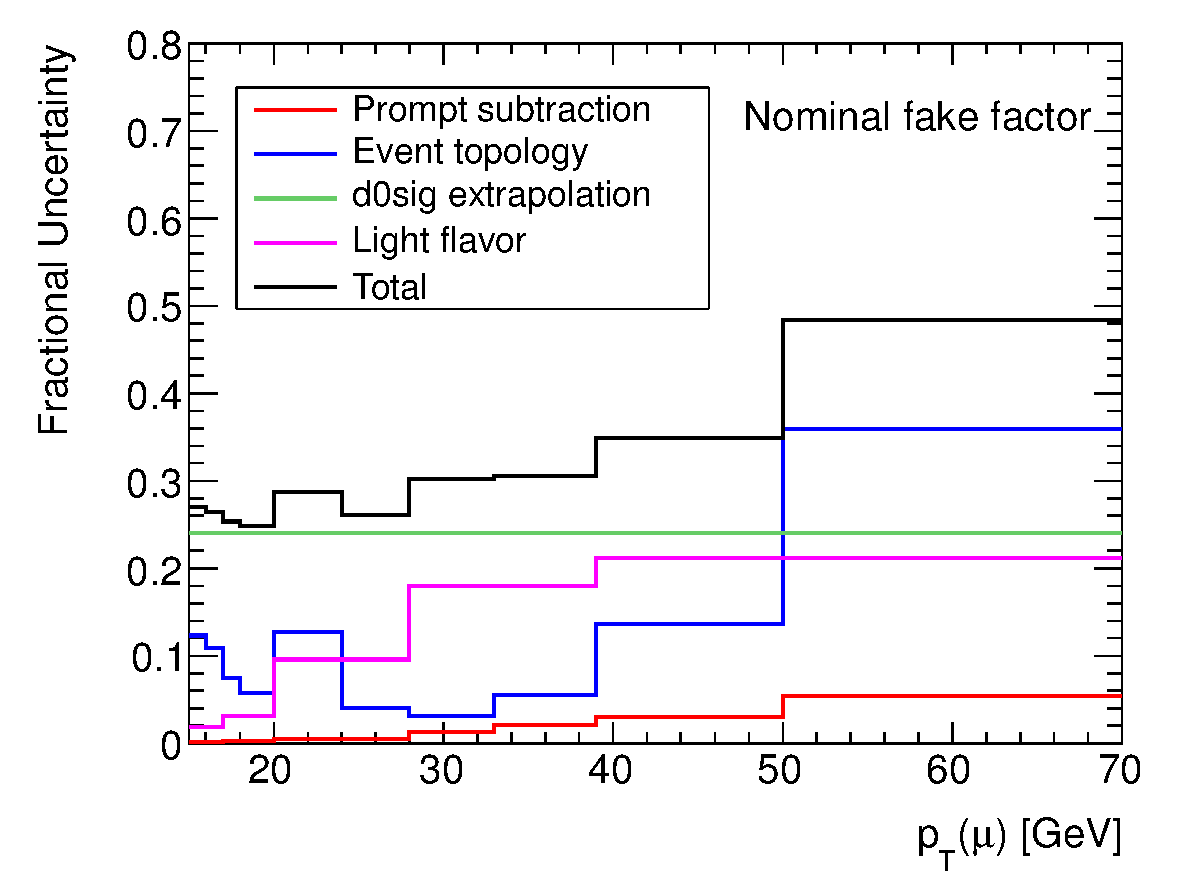
\includegraphics{figures/ch5-model-independent/MuFake_syst_nom}}
  }
  \subfloat[ Two-jet FF] {
	\resizebox{0.48\textwidth}{!}{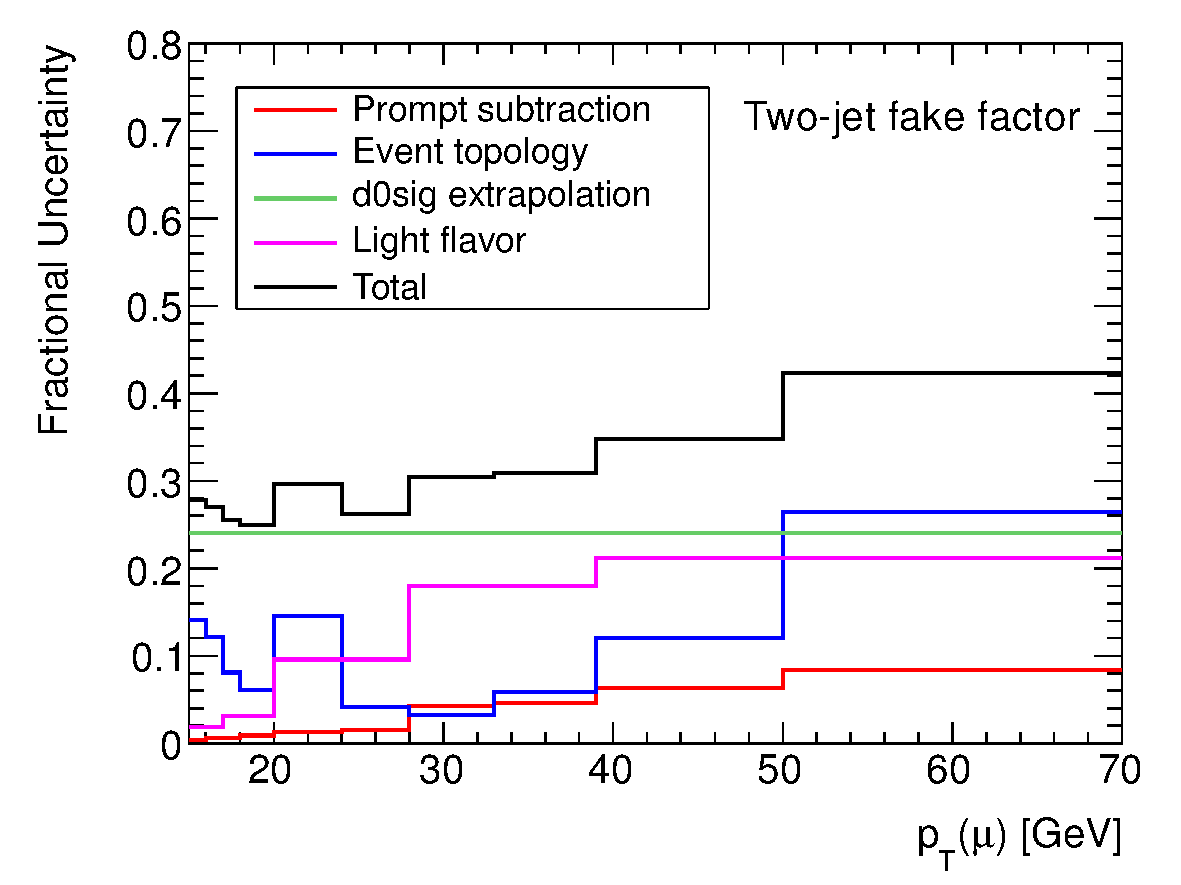
\includegraphics{figures/ch5-model-independent/MuFake_syst_2jet}}
  }
  \caption{Systematic uncertainties on muon fake factor as a function of $p_{T}(\mu)$.  The left plot shows the uncertainties for the inclusive fake factor, while the right shows the uncertainty for the two-jet fake factor.}
  \label{fig:MuFake_syst}
\end{figure}


\subsection{Application of Fake Factors}\label{sec:fake-factor-application}
Figure~\ref{fig:prompt-subtractions} shows the fake factor-weighted reducible events in the signal regions, as given by equation~\ref{eq:fake-factor-master-formula}. The estimated prompt subtractions due to $Z+\gamma$, $WZ$, $ZZ$, $t\overline{t}+V$, and $VVV^{(*)}$ events (i.e. the contributions to events with denominator objects due these irreducible background sources, rather than the intended sources of reducible background) are shown in the colored histograms. The reducible background prediction is the difference between the data points and the prompt subtraction histograms. In cases where a bin is negative after applying the prompt subtraction, the contents of that bin are set to zero, and the histogram is scaled to preserve the overall normalization. For the 4L, $Z+e$ signal region, the overall normalization is negative and consistent with zero, so the background is neglected in this region. 

The uncertainty on the background prediction is the combination of two components: the systematic uncertainties on the electron and muon fake factors, and the statistical uncertainties due to finite events with denominator objects. As described in section~\ref{sec:systematic-uncertainties}, the fake factor uncertainties constitute their own component, while the statistical uncertainties are contained in the ``Monte Carlo statistics'' component. 

\begin{figure}[h]
	\centering
	\subfloat[ Inclusive SR, $Z+e$] {
		\resizebox{3in}{!}{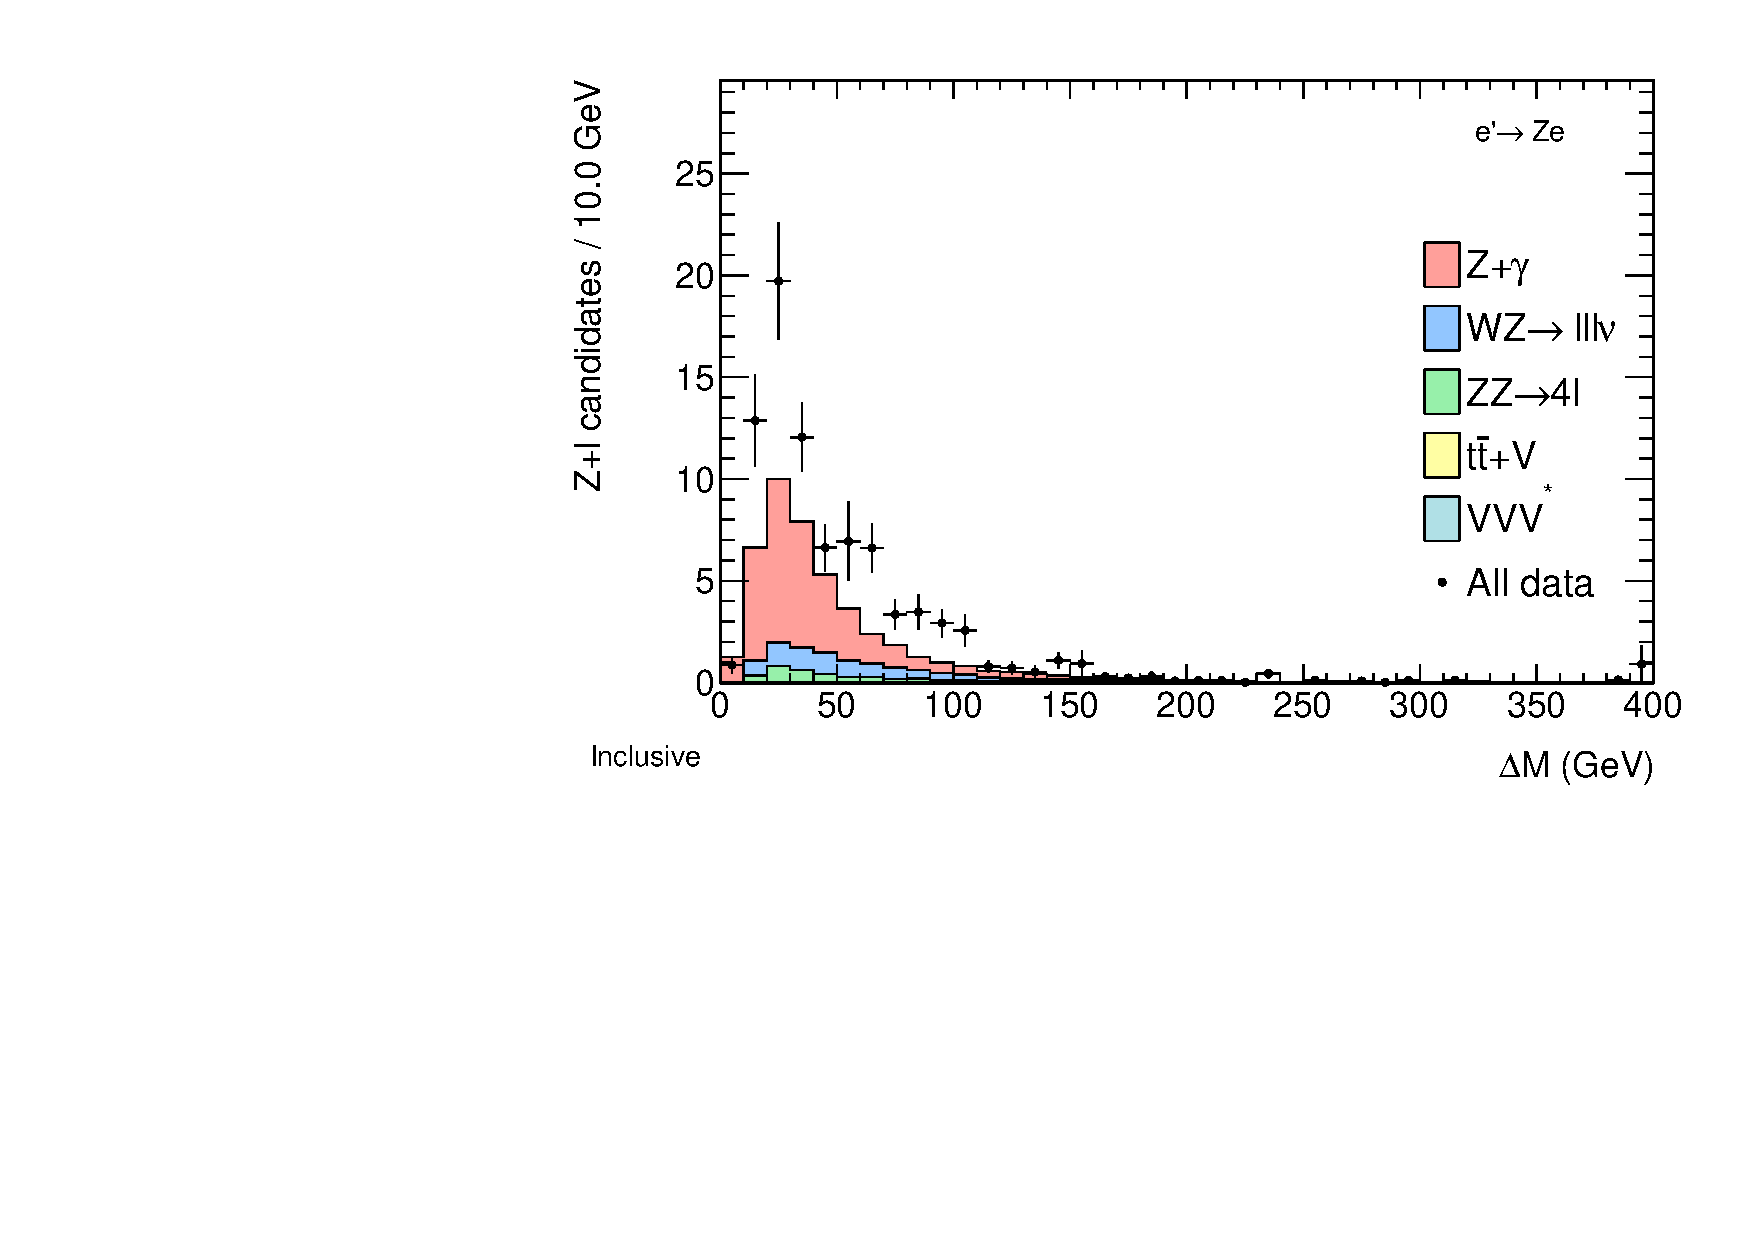
\includegraphics{figures/ch5-model-independent/c_output_reducible_DeltaM_Ze_InclusiveNoM3L}}
	}
	\subfloat[ Inclusive SR, $Z+\mu$] {
		\resizebox{3in}{!}{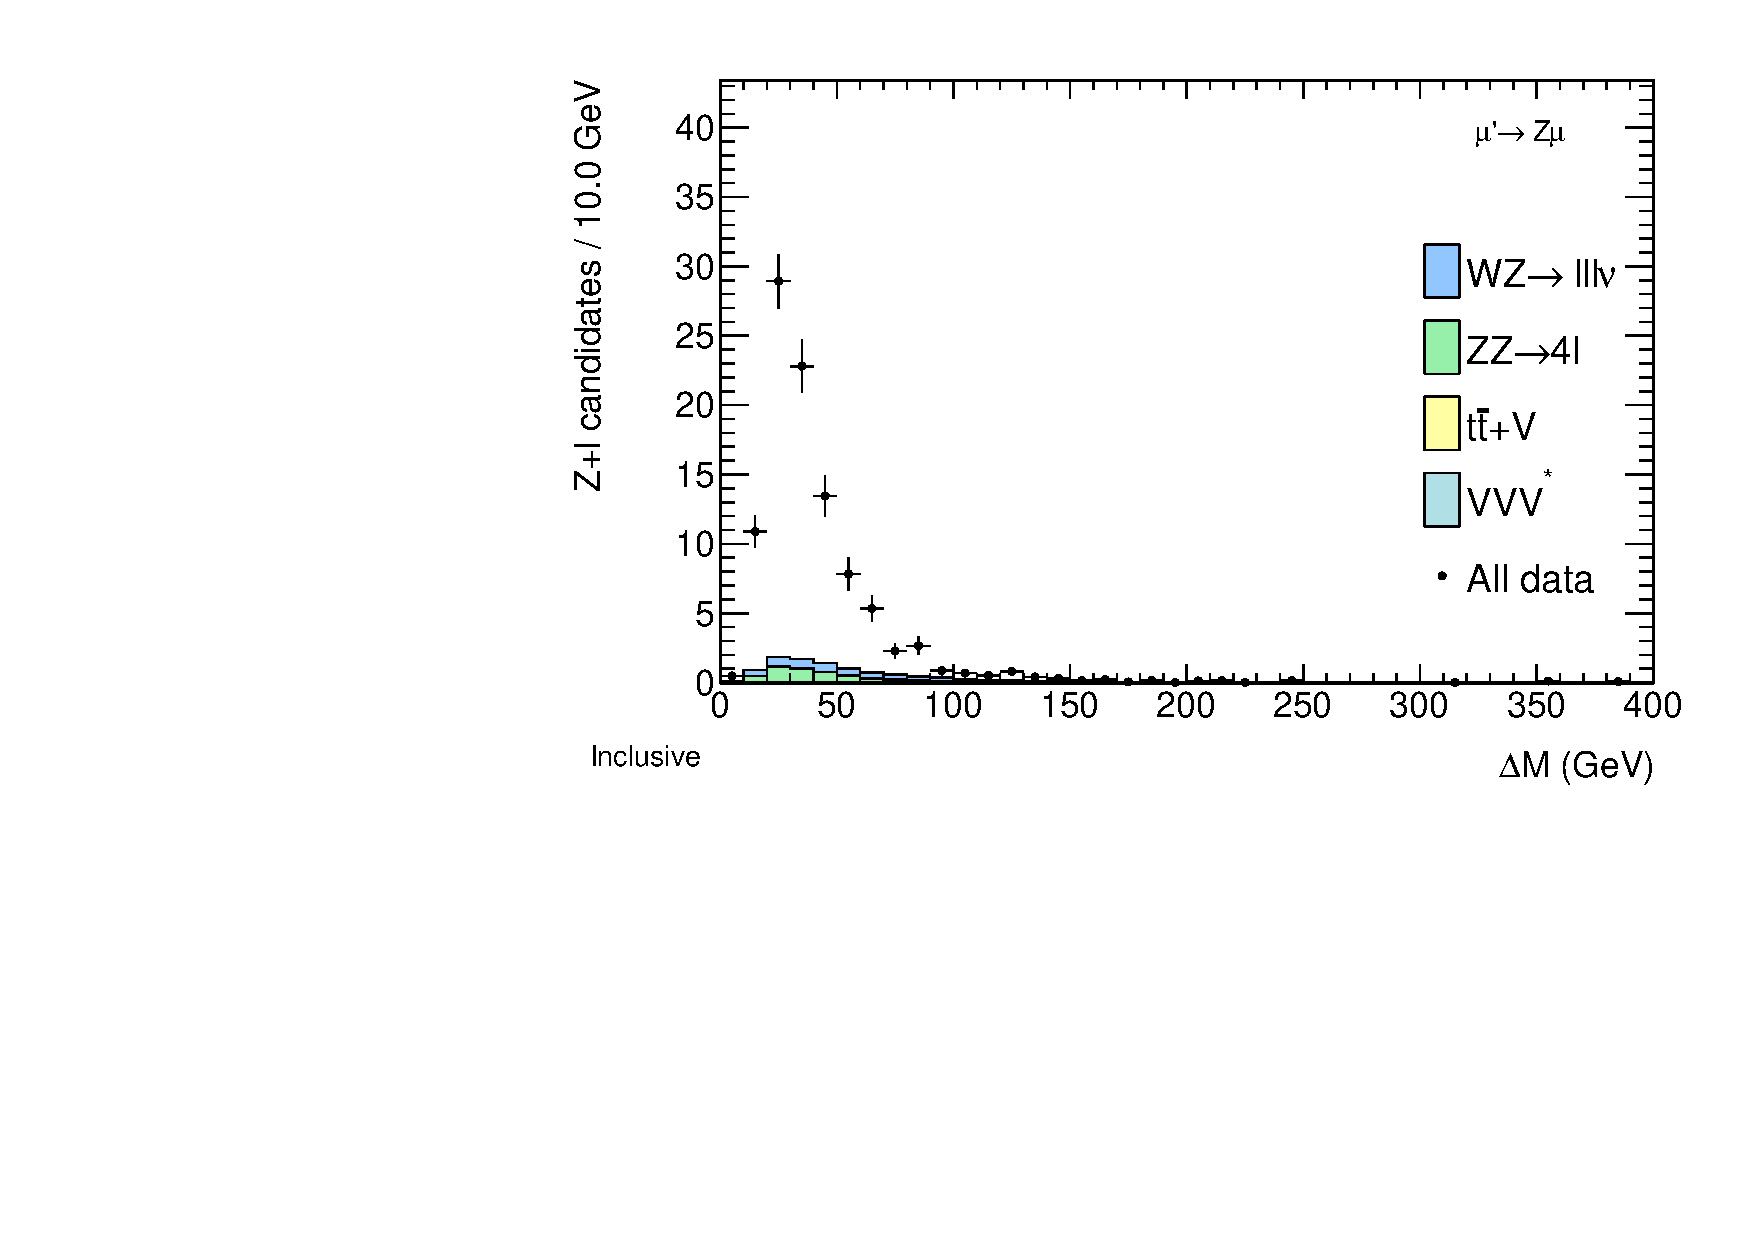
\includegraphics{figures/ch5-model-independent/c_output_reducible_DeltaM_Zmu_InclusiveNoM3L}}
	} \\
	\subfloat[ 4L SR, $Z+e$] {
		\resizebox{3in}{!}{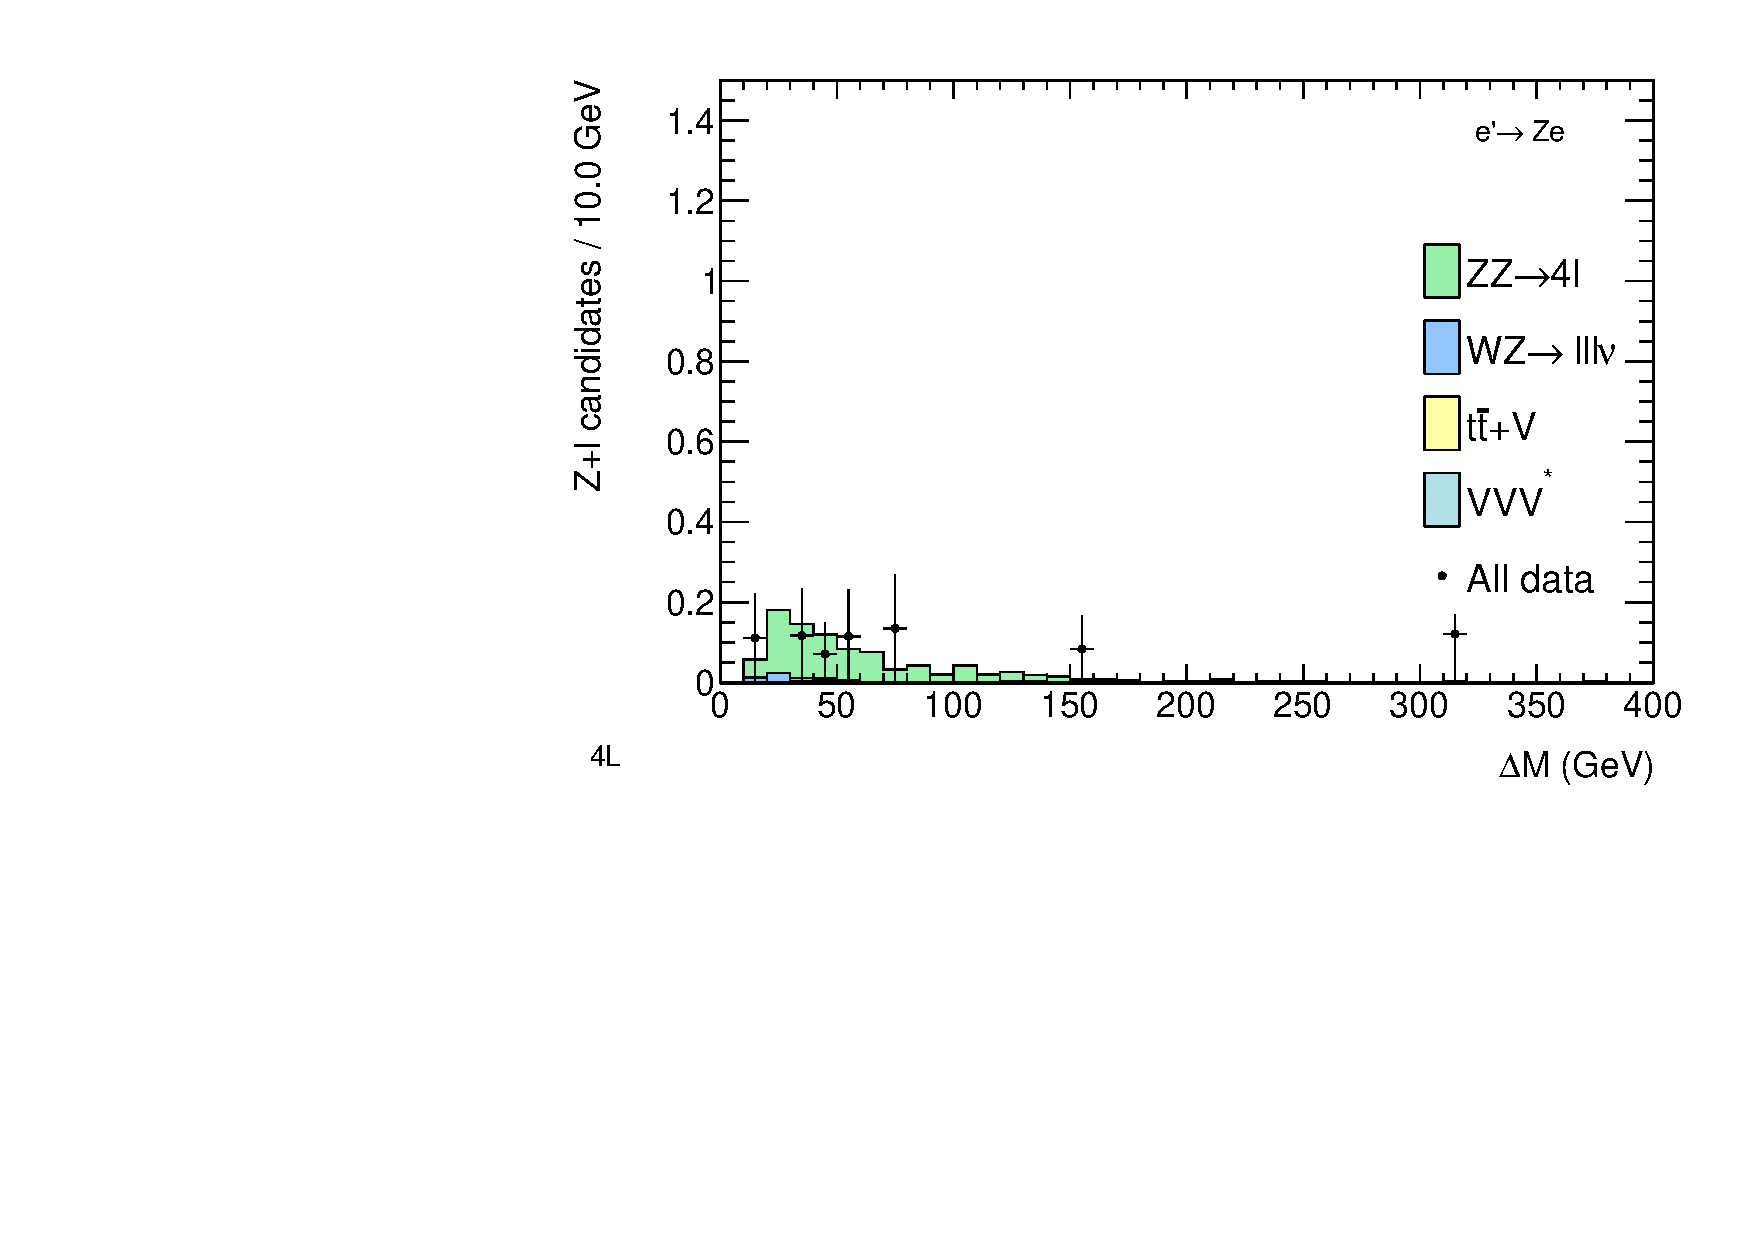
\includegraphics{figures/ch5-model-independent/c_output_reducible_DeltaM_Ze_FourLNoM3L}}
	}
	\subfloat[ 4L SR, $Z+\mu$] {
		\resizebox{3in}{!}{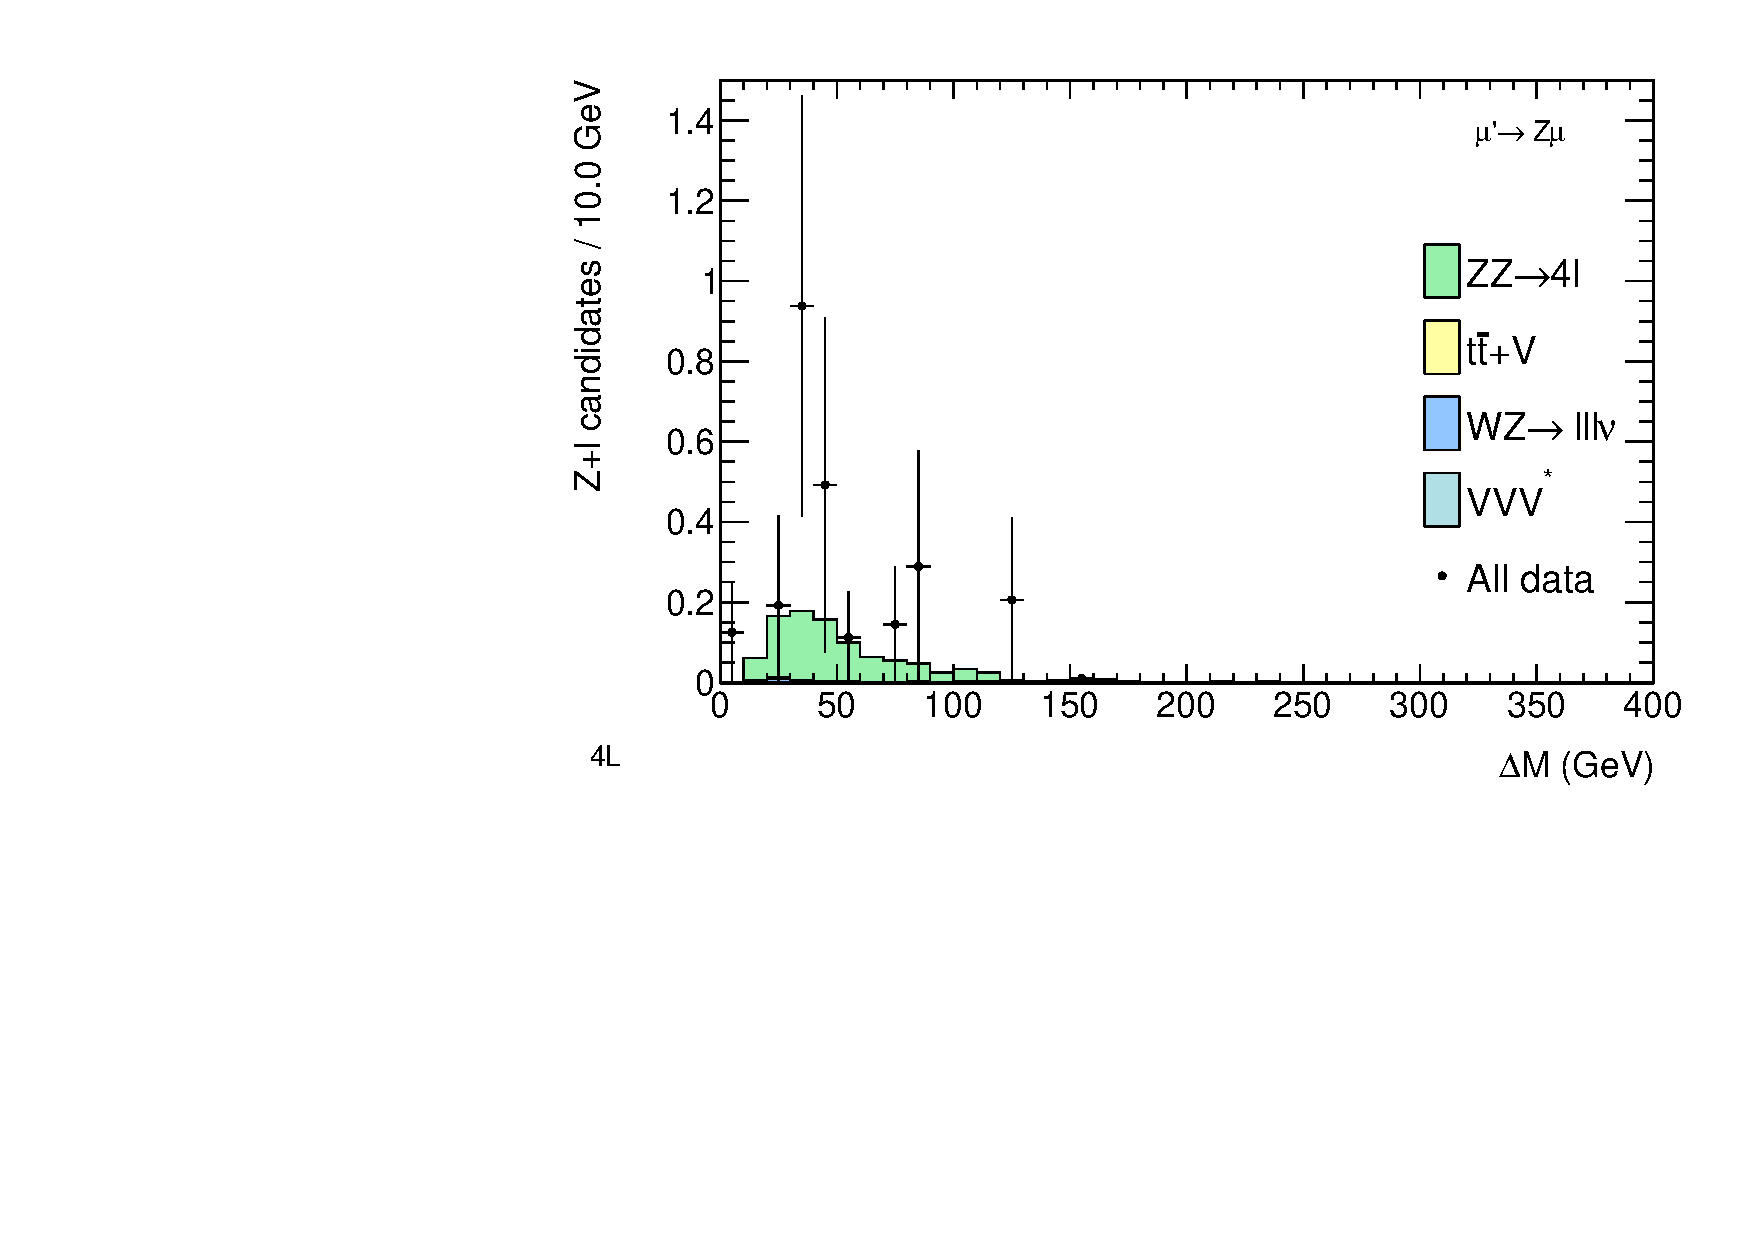
\includegraphics{figures/ch5-model-independent/c_output_reducible_DeltaM_Zmu_FourLNoM3L}}
	} \\
	\subfloat[ 3L+dijet SR, $Z+e$] {
		\resizebox{3in}{!}{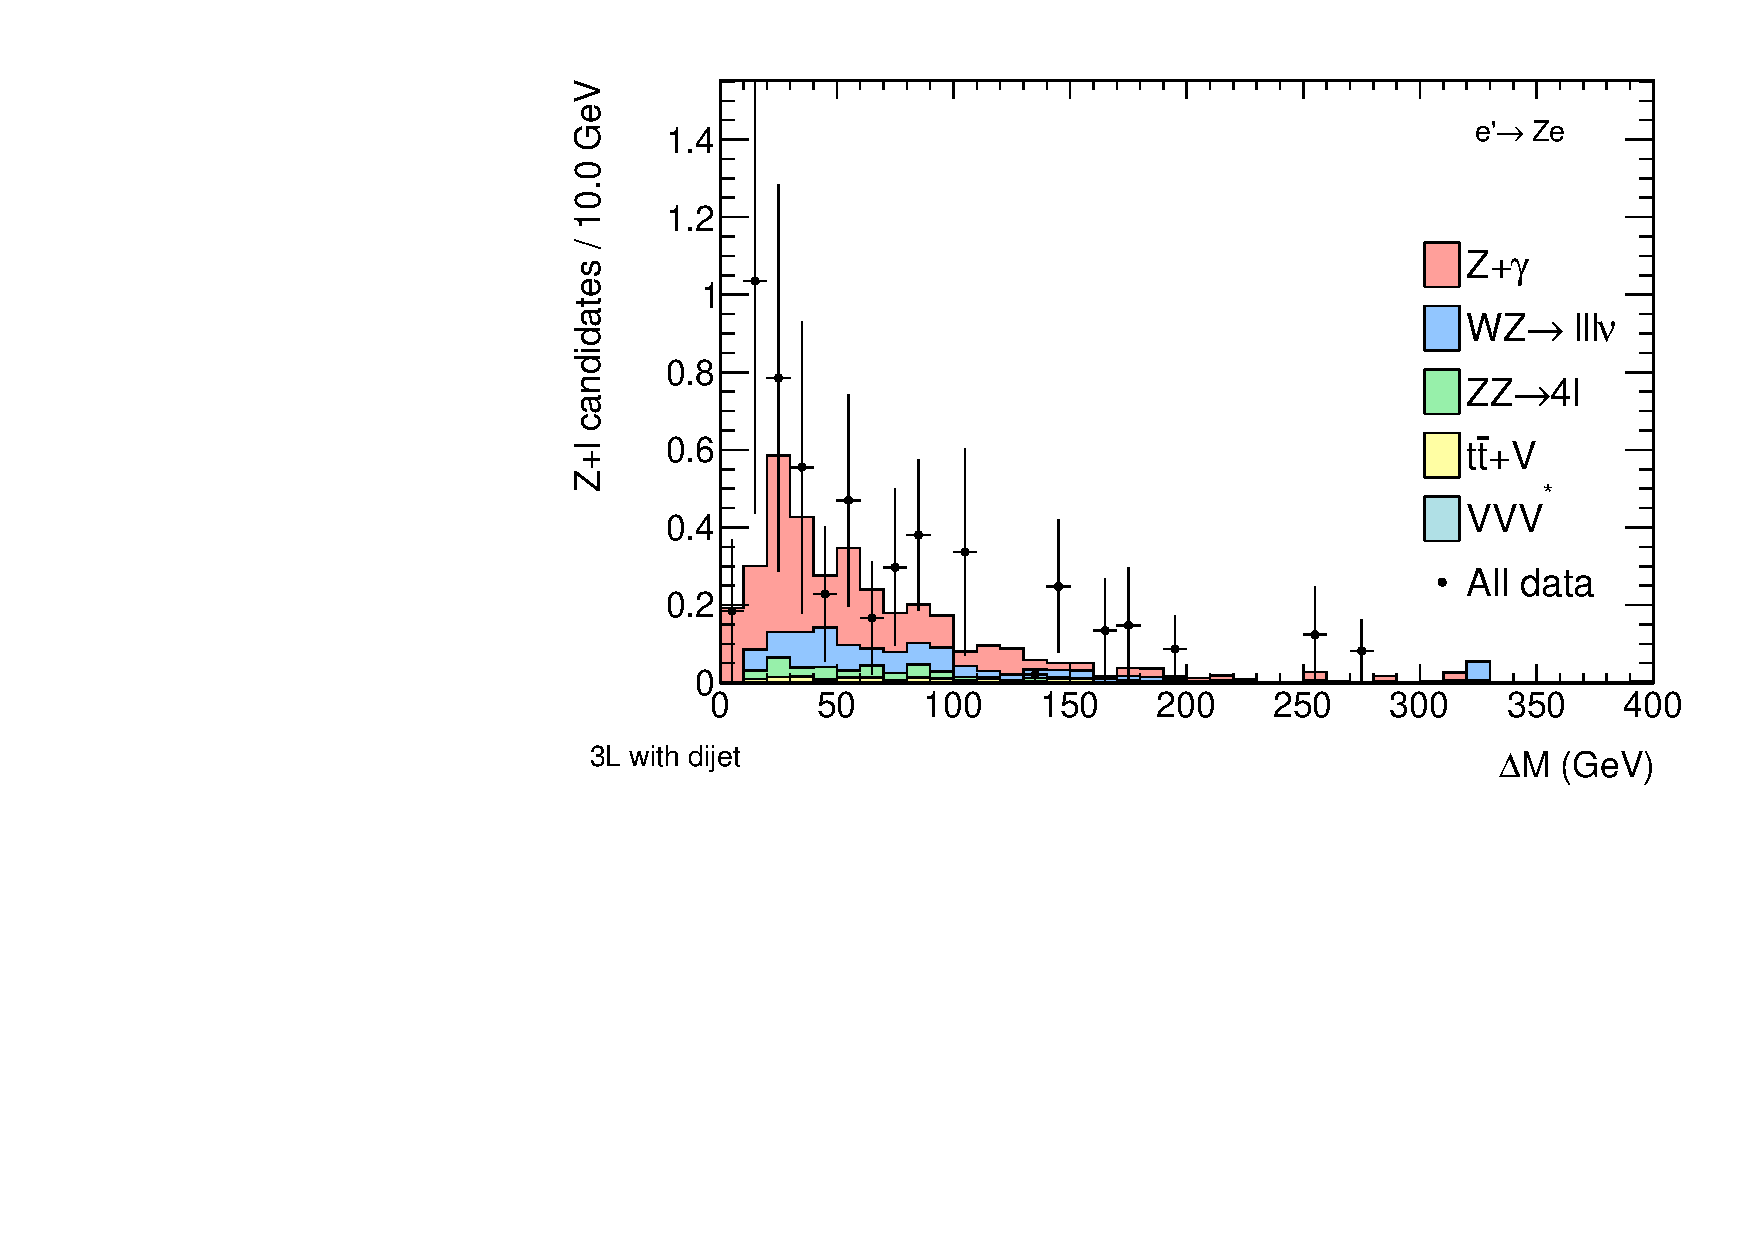
\includegraphics{figures/ch5-model-independent/c_output_reducible_DeltaM_Ze_ThreeLDijetNoM3L}}
	}
	\subfloat[ 3L+dijet SR, $Z+\mu$] {
		\resizebox{3in}{!}{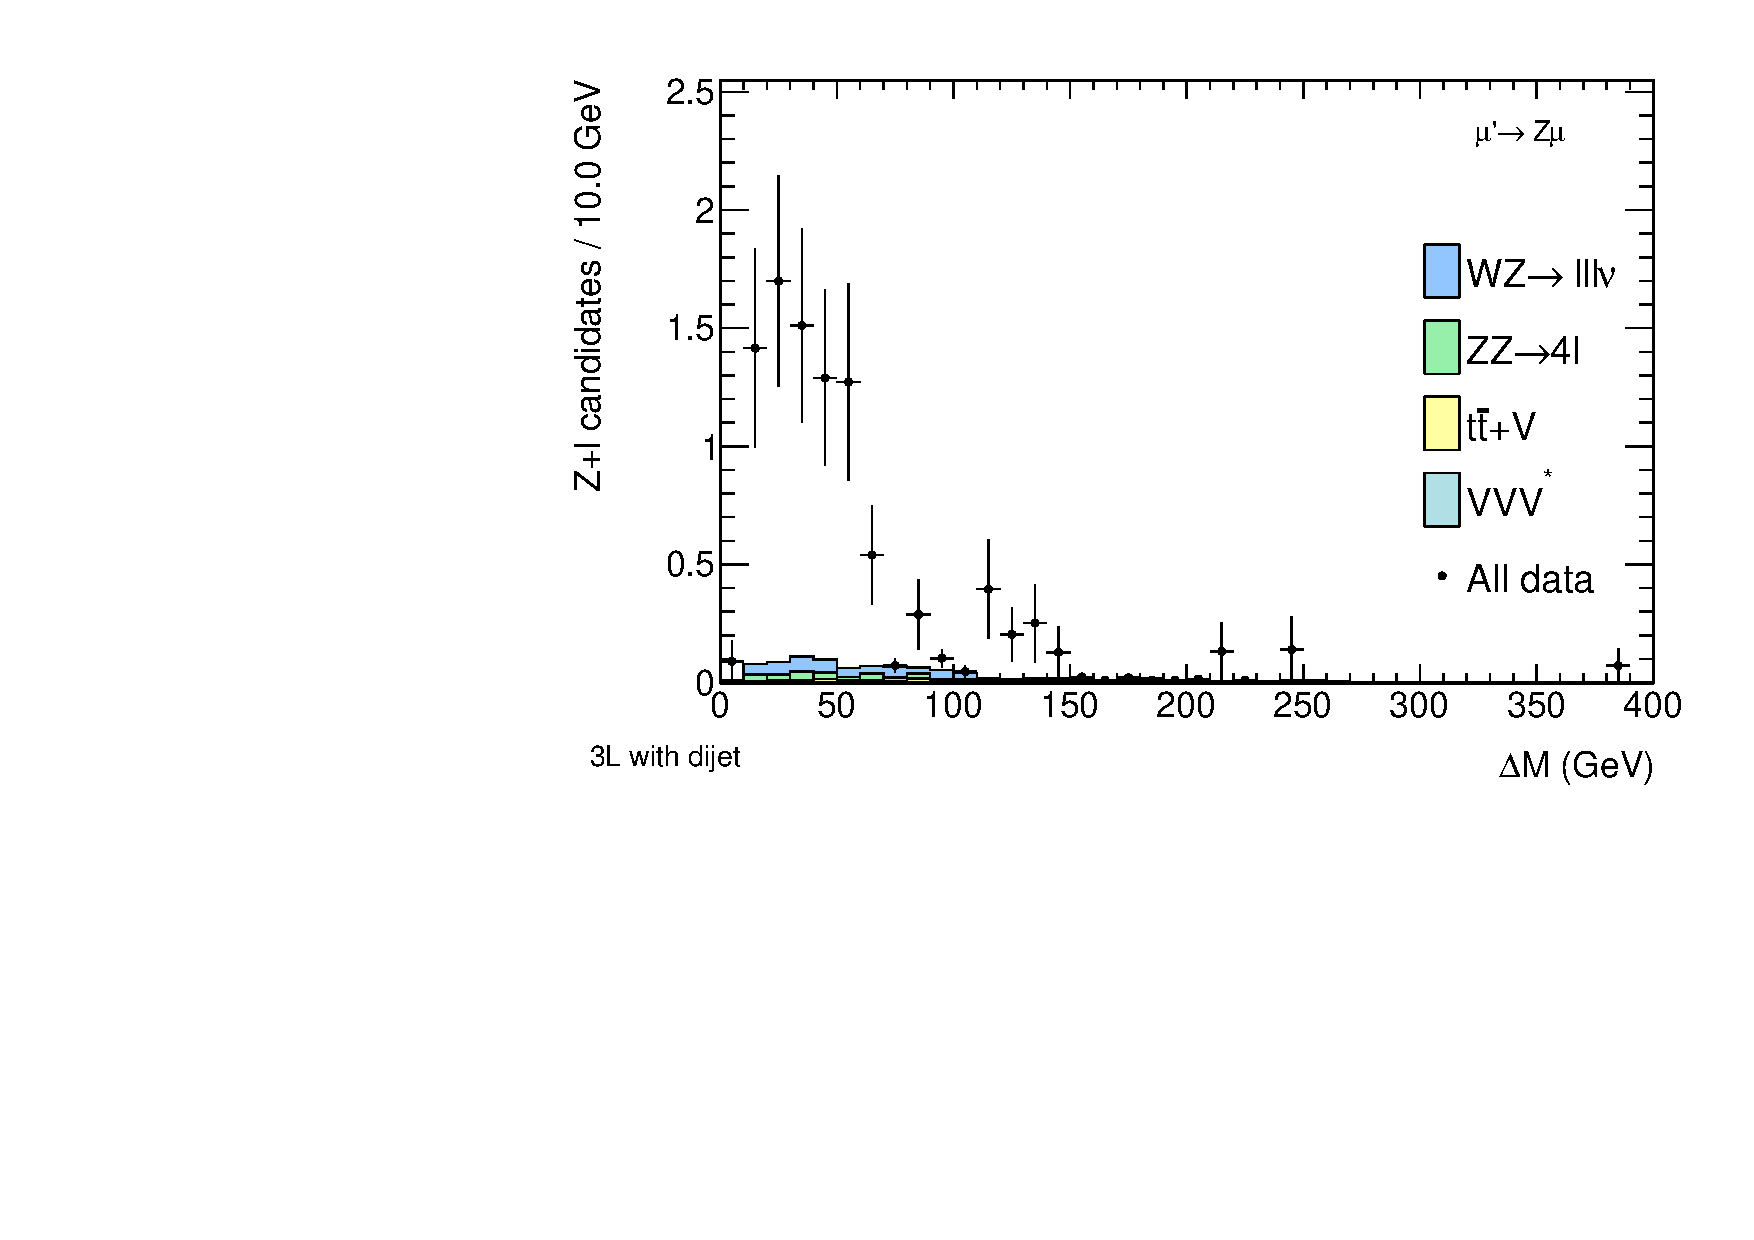
\includegraphics{figures/ch5-model-independent/c_output_reducible_DeltaM_Zmu_ThreeLDijetNoM3L}}
	} \\
	\caption{Fake factor-weighted data events and prompt subtractions. The reducible background prediction is the difference between the data points and the prompt subtraction colored histograms.}
	\label{fig:prompt-subtractions}
\end{figure}

\subsubsection{Tau Lepton Fakes}\label{sec:model-independent-ff-tau}
The detector signature of hadronically decaying tau leptons, consisting of a jet with one or more associated tracks, is not as distinctive as the signature of electrons and muons. Differentiating between jet, which are copiously produced in proton-proton collisions, and hadronically decaying tau leptons is difficult, and accordingly the reducible backgrounds in the 2L$+\tau_{\mathrm{had}}$ categories tend to be much larger than those in the 3L categories. 

\textcolor{red}{Lots of work to do here, to avoid copying and pasting PO's work!}

As taus can decay hadronically, their detector signature is not as distinctive as the one
associated with electrons and muons.  Therefore, jets, which are produced in abundance in
proton-proton collisions, are the main source of tau fakes, leading to large expected
fake-rates.  As the tau identification algorithms use multi-variate discriminants based on
calorimeter shower shapes and tracking information, the fake efficiency is strongly
dependent on the jet fragmentation. This in turn introduces a dependency of the fake-rates
on the parton initiating the jet (gluon, light-quark or heavy-quark).

Consequently, the fake-factors are less sensitive to the jet flavour if a tighter
efficiency working point is chosen for the denominator (as some shower shape requirements
are already applied).  However, it is important to still choose a working point that is
loose enough so that the denominator statistics are sufficiently large. A study of the
flavour-dependency of the fake-factors was performed in simulation samples.  For each jet
faking a $\tau$, the largest $p_{T}$ truth-particle present inside of the $\tau$
reconstruction cone was taken as an estimator of the parton initiating the jet.
Different denominator selections were chosen as a function of the existing loose
identification working point.  Denominators failing the \texttt{BDT-Medium} selection while
having a \texttt{BDTScore} larger than 0.7, 0.8, 0.9 or 1.0 $\times$ \texttt{BDTScore$_{Loose}$}
were all studied (where \texttt{BDTScore$_{Loose}$} is the $p_{T}$ dependent cut on the \texttt{  BDTScore} used by the $\tau$ identification algorithm).  Illustratively, each sequential
cut tightening denominator score reduces the statistics by a factor of roughly 2.  In the
end, the minimal threshold of 0.9 $\times$ \texttt{BDTScore$_{Loose}$} was chosen as it
offered a greatly reduced sensitivity to the flavour of the initiating parton in the jet,
while still offering large enough statistics for the sample. Further tightening of the cut
provided little improvement in flavour dependence. Using a $p_{T}$-dependent denominator
requirement ensures that the prompt efficiency is the same for all denominator taus, while
lowring the fake-factor dependent on $p_{T}$.

%A consequence of this choice of denominator is that the \met\ is incorrectly
%calibrated in events with denominator taus.  This is corrected in the analysis by
%modifying the \verb.RefJet. and \verb.RefTau. terms of \verb.MET_RefFinal. to use the tau
%energy instead of the jet energy.

The fake-factors are nominally parameterized as a function of the $p_{T}$ and $|\eta|$ of the
tau candidate, binned in 2 dimensions to preserve correlations. An additional scaling
correction is applied as a function of the highest \texttt{MV1} $b$-tagging weight of any jet
in the event.  The former two target dependencies associated with the jet shower shapes as a
function of kinematics and detector homogeinity.  The latter is taken to account for the
heavy-flavour component.

\subsubsection{Fake Factor Measurement}\label{sec:model-independent-ff-tau-measurement}

It is also important to measure the fake-factors in a sample which is expected to have a
similar flavour composition as the signal regions used (the majority of trilepton events
with a fake tau are expected to come from electroweak production with an associated jet
faking the tau, for example $Z$ + jets events).  This is particularly important as no
observable can be used to directly and accurately classify each fake taus as potentially
gluon- or quark-initiated.
 
While the tau fake-factors were measured in the past from a $\gamma + $ jets sample, the
approach chosen for this iteration of the analysis is different.  
%Due to the increased
%pile-up conditions of the 2012 run, the purity of the photon sample is greatly
%compromised, leading to a larger contribution from multijet events, which then introduces
%a larger contribution from gluon-initiated jets, biasing the fake-factors.  
%Furthermore,
The low $p_{T}$ photon triggers were heavily prescaled during the 2012 run, limiting the
statistics available to measure fake-factors at low $p_{T}$ values.  Instead, a $W$ + jets
sample is used due to its high statistics and similar final-state kinematics.  A leading
numerator muon is required to be reconstructed as a tag (along with the associated trigger
requirement), and the fake-factors are then measured from the probe tau candidates.  No
other requirements are made on the events.  Alternatively, selection requirements could be
made to reject the main source of $\tau_{\mathrm{had}}$ prompts ($Z\rightarrow
\tau_{\mu}\tau_{\mathrm{had}}$), but such requirements can potentially introduce a bias on
the fake-factors (for example, introducing a same-sign requirement is expected to
drastically reduce the quark-initiated jet contribution).  Instead, the contribution from
prompt $\tau_{\mathrm{had}}$ is subtracted directly from Monte Carlo simulations.  The two
non-negligible contributions come from $Z$ + jets and $t\bar{t}$ events.

\begin{figure}
\centering 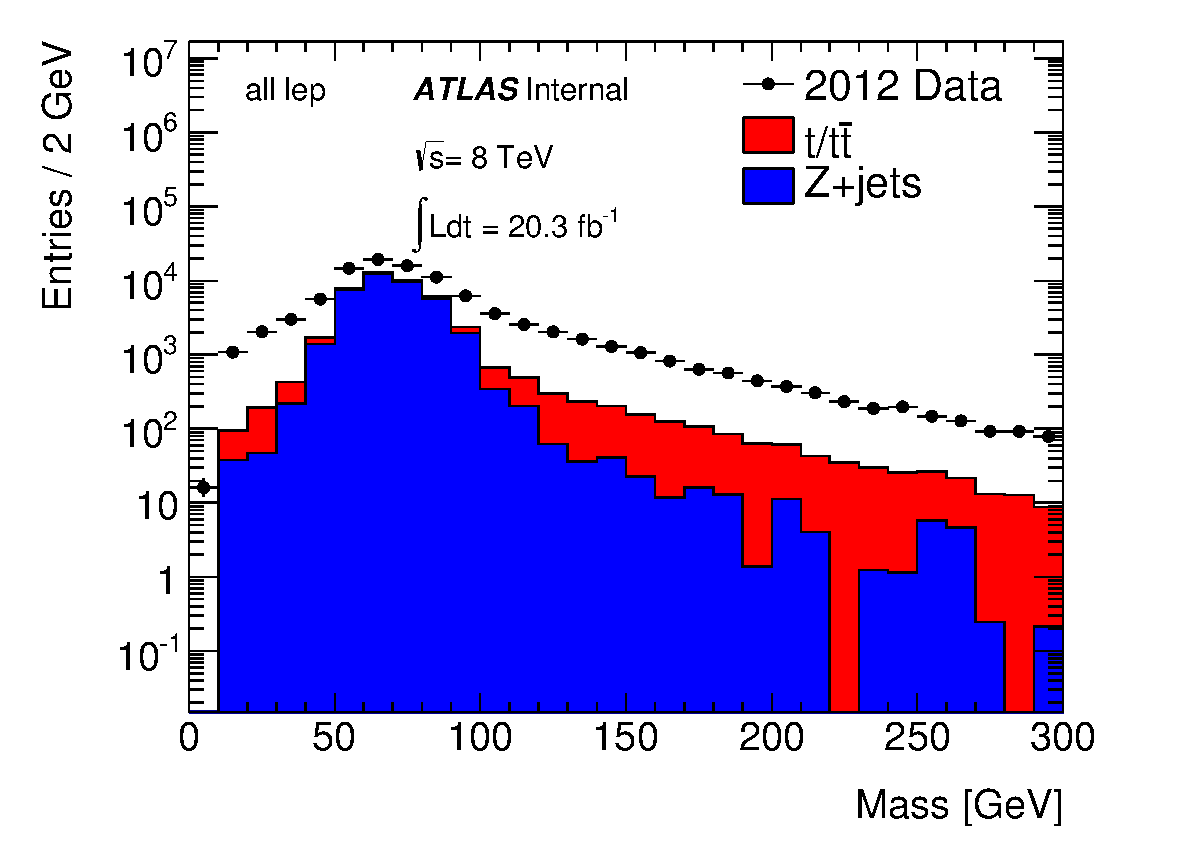
\includegraphics[width=0.48\textwidth]{figures/ch5-model-independent/TauFakes_NumM}
\centering 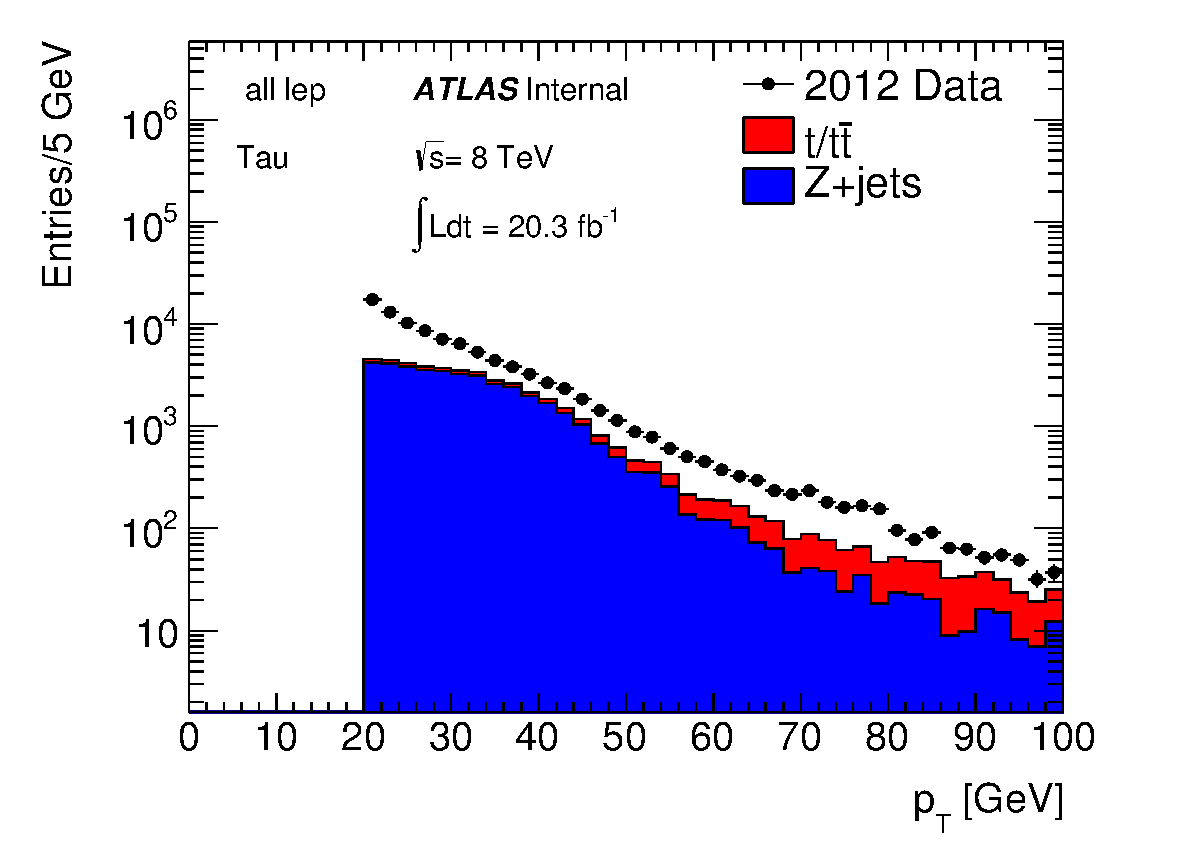
\includegraphics[width=0.48\textwidth]{figures/ch5-model-independent/TauFakes_NumPt}
\centering 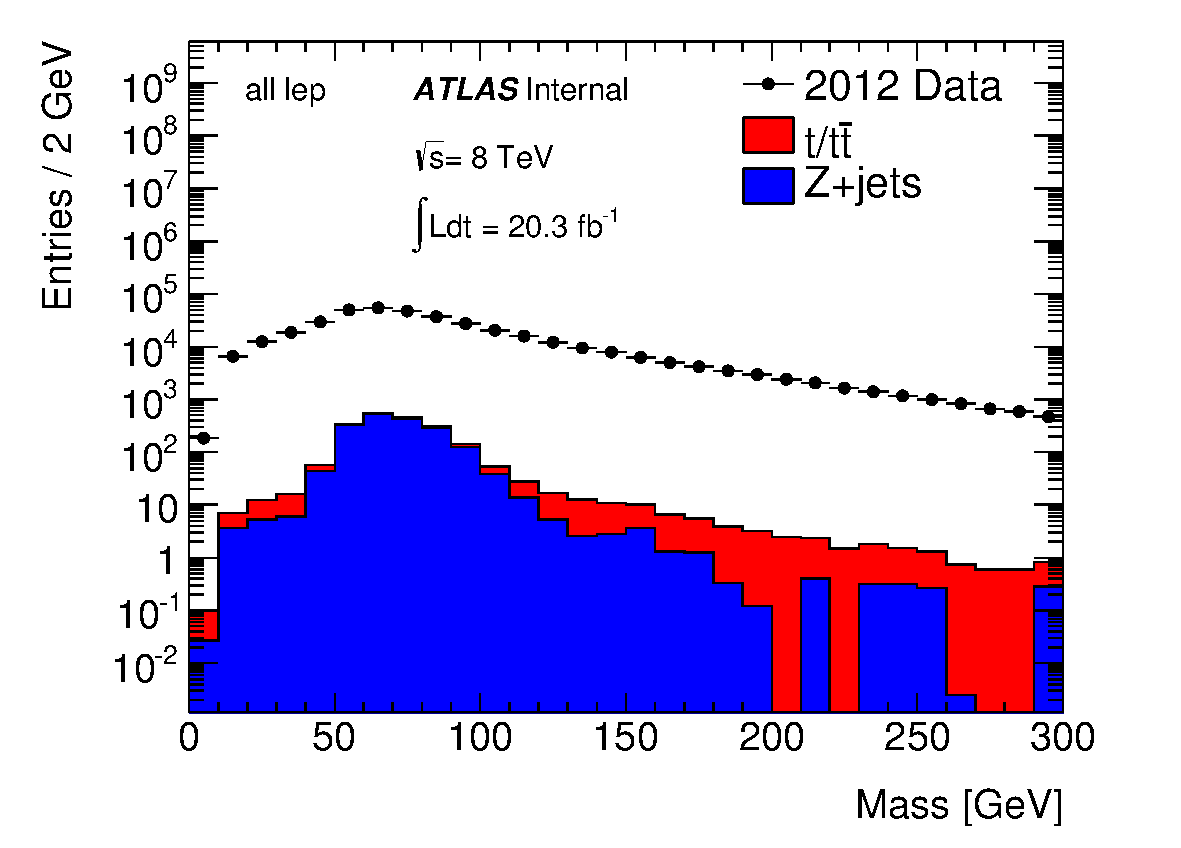
\includegraphics[width=0.48\textwidth]{figures/ch5-model-independent/TauFakes_DenM}
\centering 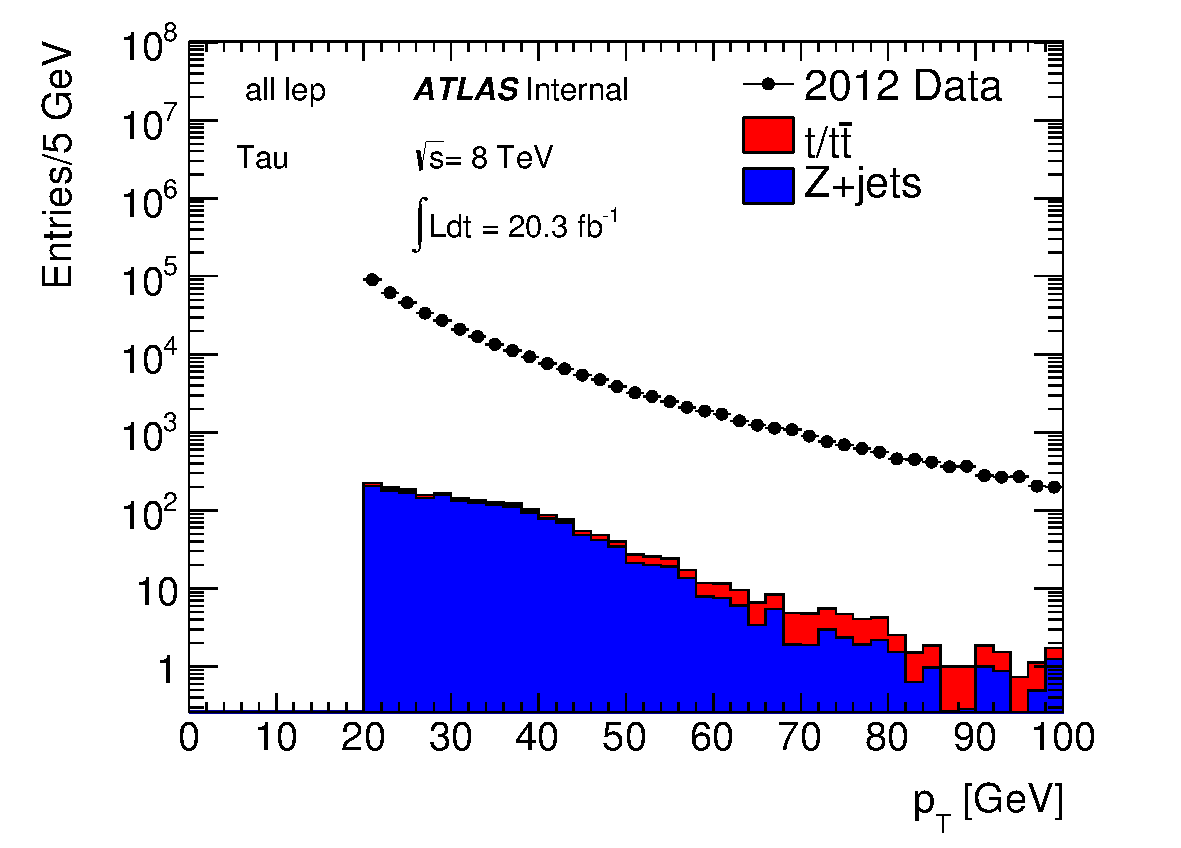
\includegraphics[width=0.48\textwidth]{figures/ch5-model-independent/TauFakes_DenPt}
\caption{\label{fig:taufakeprompt} Invariant mass of the muon and tau pair (left) and
  $p_{T}$ of the tau candidate (right), for the numerator (top) and denominator selections
  (down).  The prompt contribution estimated from MC simulations is shown along with the
  measured data.}
\end{figure}

\begin{figure}
\centering 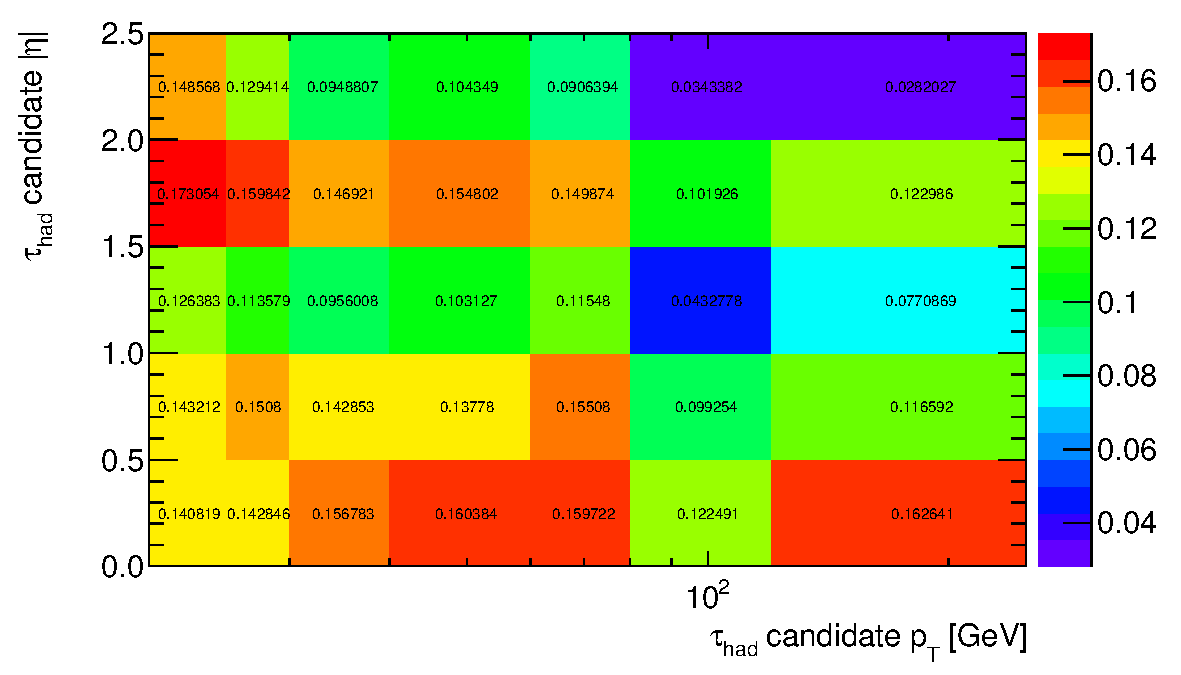
\includegraphics[width=0.48\textwidth]{figures/ch5-model-independent/TauFakes_FFPt}
\centering 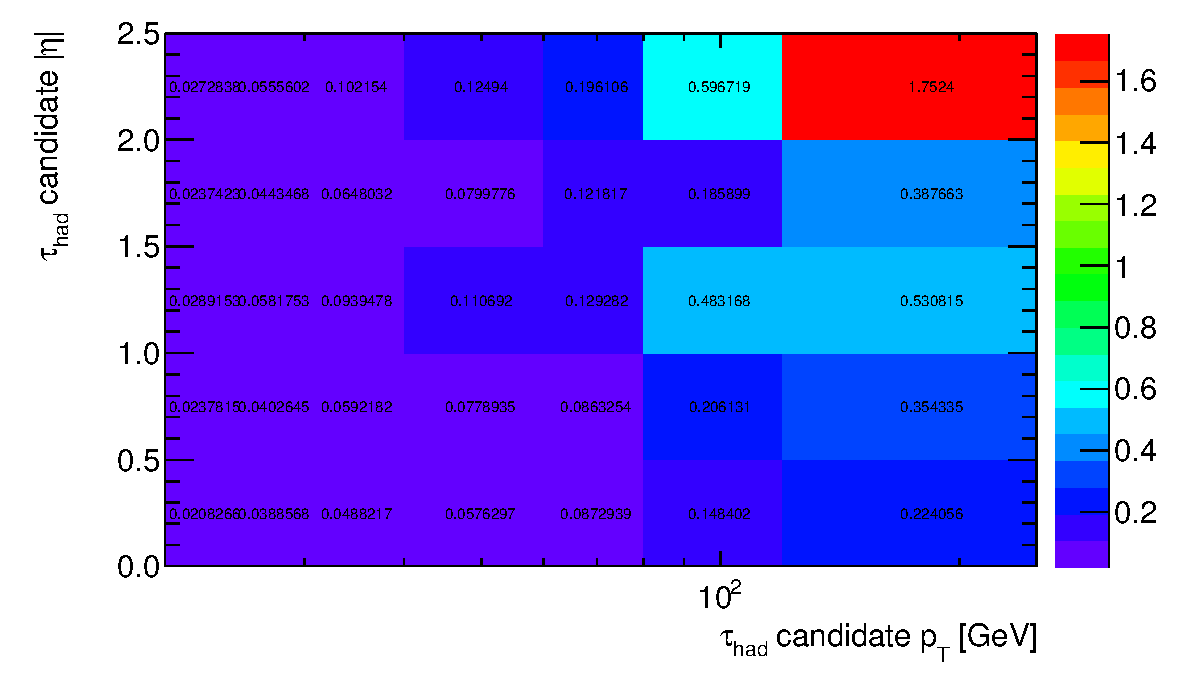
\includegraphics[width=0.48\textwidth]{figures/ch5-model-independent/TauFakes_FFEta}
\centering 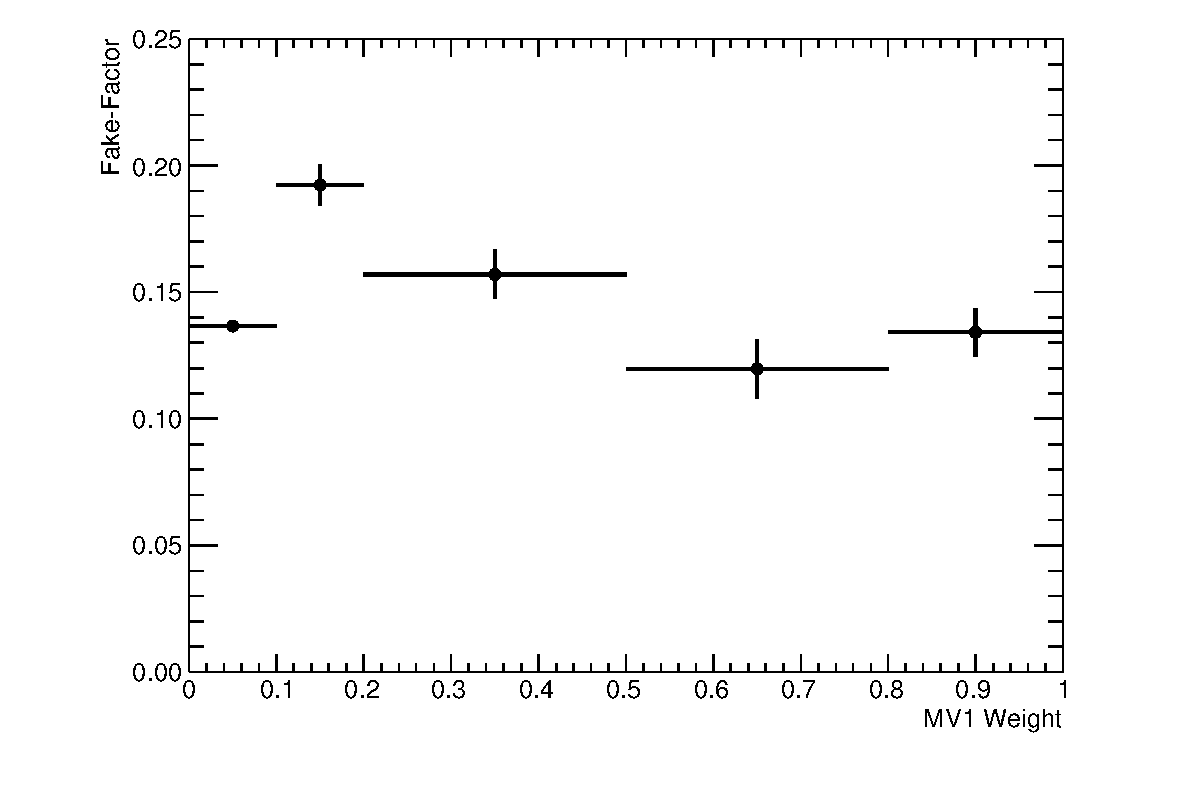
\includegraphics[width=0.48\textwidth]{figures/ch5-model-independent/TauFakes_FFMV1}
\caption{\label{fig:taufakefactors} Fake-factors binned in $p_{T}$ and $|\eta|$ (left) and
  their associated statistical uncertainty (right). The extra scaling as a function of MV1
  weight is also shown (bottom).  These fake-factors were derived in $W$ + jets
  events. The prompt contribution has been subtracted using MC predictions.}
\end{figure}

Figure~\ref{fig:taufakeprompt} shows sample data distributions for the numerator and
denominator tau candidates, along with the prompt contribution which must be subtracted
when calculating the fake-factors. Figure~\ref{fig:taufakefactors} shows the obtained
fake-factors.

\subsubsection{Systematic Uncertainties}\label{sec:model-independent-ff-tau-systematics}

Various studies have been carried out to estimate the systematic uncertainties associated
with the tau fake estimates.  The main considered sources of uncertainties are the following:

\begin{itemize}
\item Uncertainties on the MC prompt estimates
\item Uncertainties associated with the binning choice
%\item Dependency of the fake-factors of the $W$ + jets selection
\item Flavour dependence of the fake-factors (gluon, light-quarks, heavy-quarks)
\end{itemize}

For the prompt estimates, the normalization of the MC samples have been fluctuated by
their associated uncertainties (as listed in~\ref{s:syst}).  This results in variations
between 5\% and 17\%, being the largest in the 30-40 GeV $p_{T}$ range (where the prompt
subtraction is the largest due to the $Z$ sample kinematics).

To estimate the effect of the binning on the fake estimates, a closure test is used.  The
fake-factors are re-applied to the same sample they were derived from.  The results of
this test are shown in figure~\ref{fig:tauclosure}.  Excellent agreement is seen, and a
systematic of 5\% is attributed to this effect.

\begin{figure}
\centering 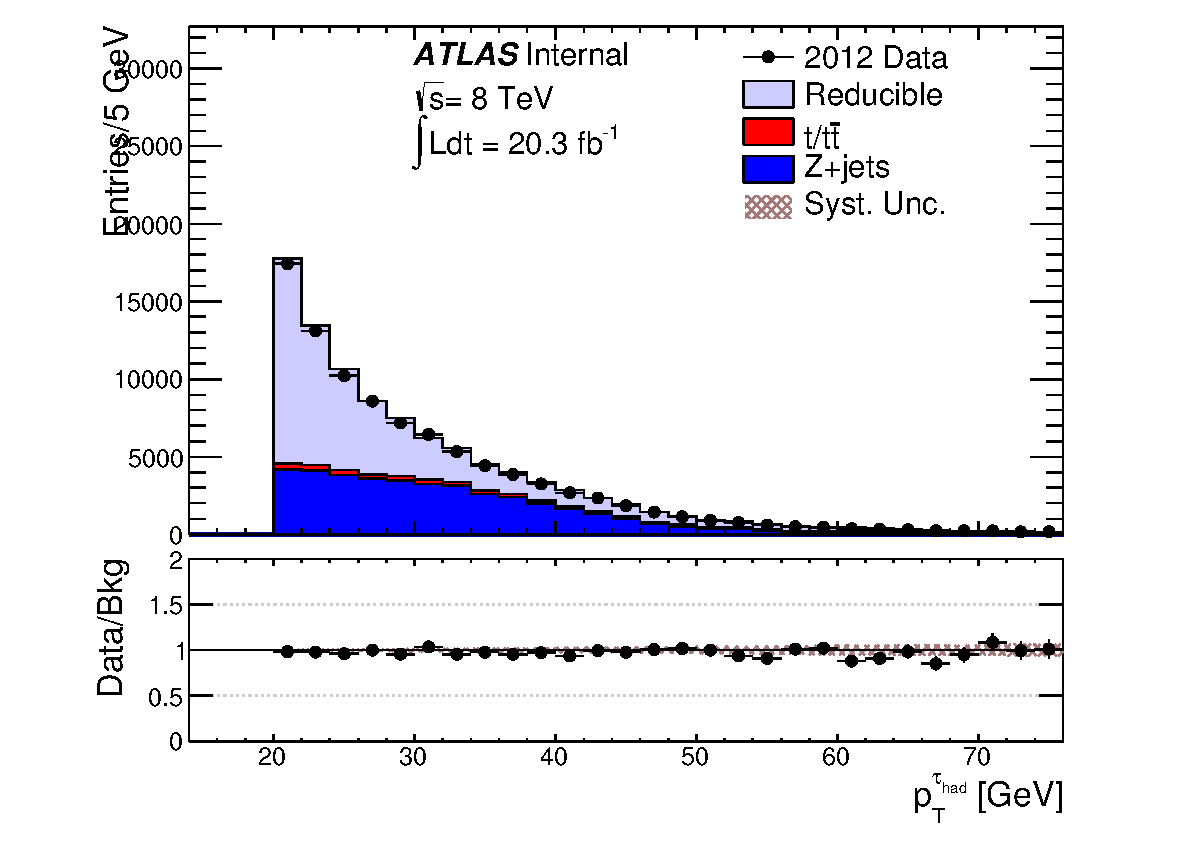
\includegraphics[width=0.48\textwidth]{figures/ch5-model-independent/TauFakes_ClosurePt}
\centering 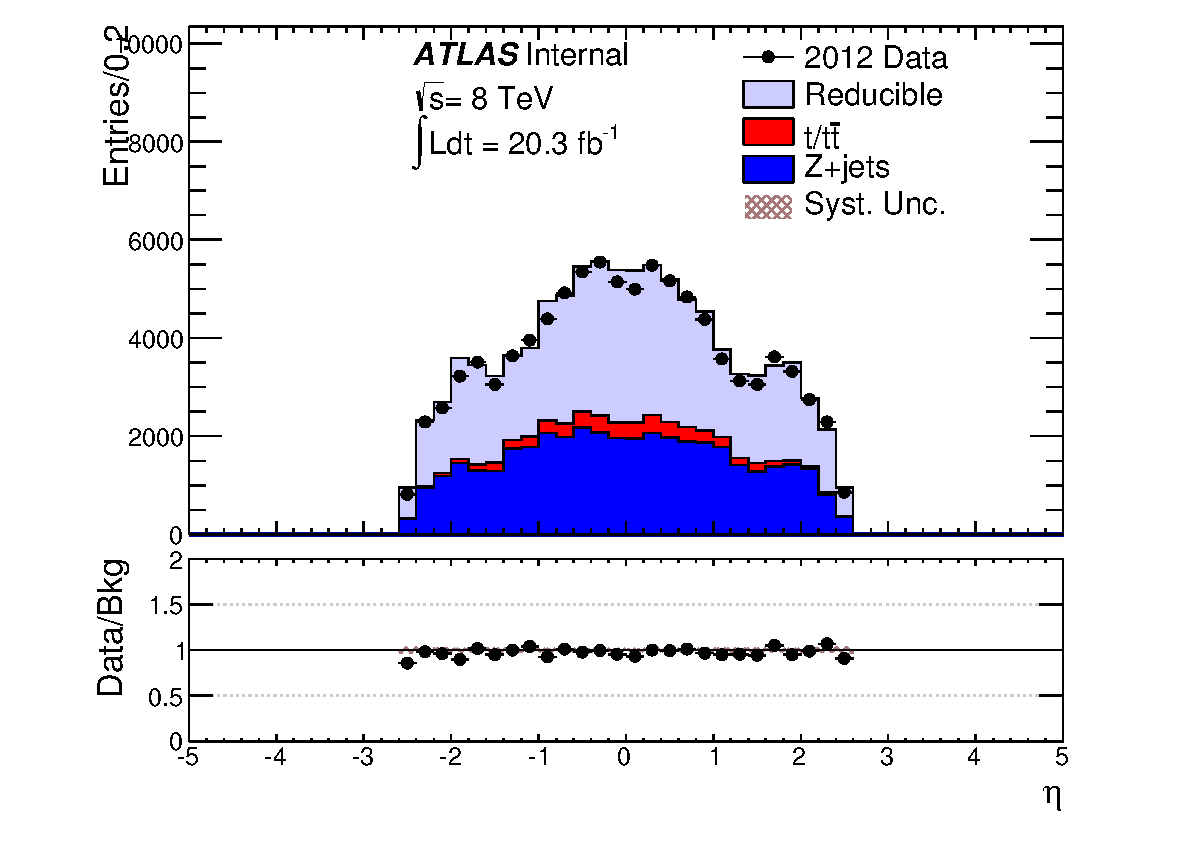
\includegraphics[width=0.48\textwidth]{figures/ch5-model-independent/TauFakes_ClosureEta}
\centering 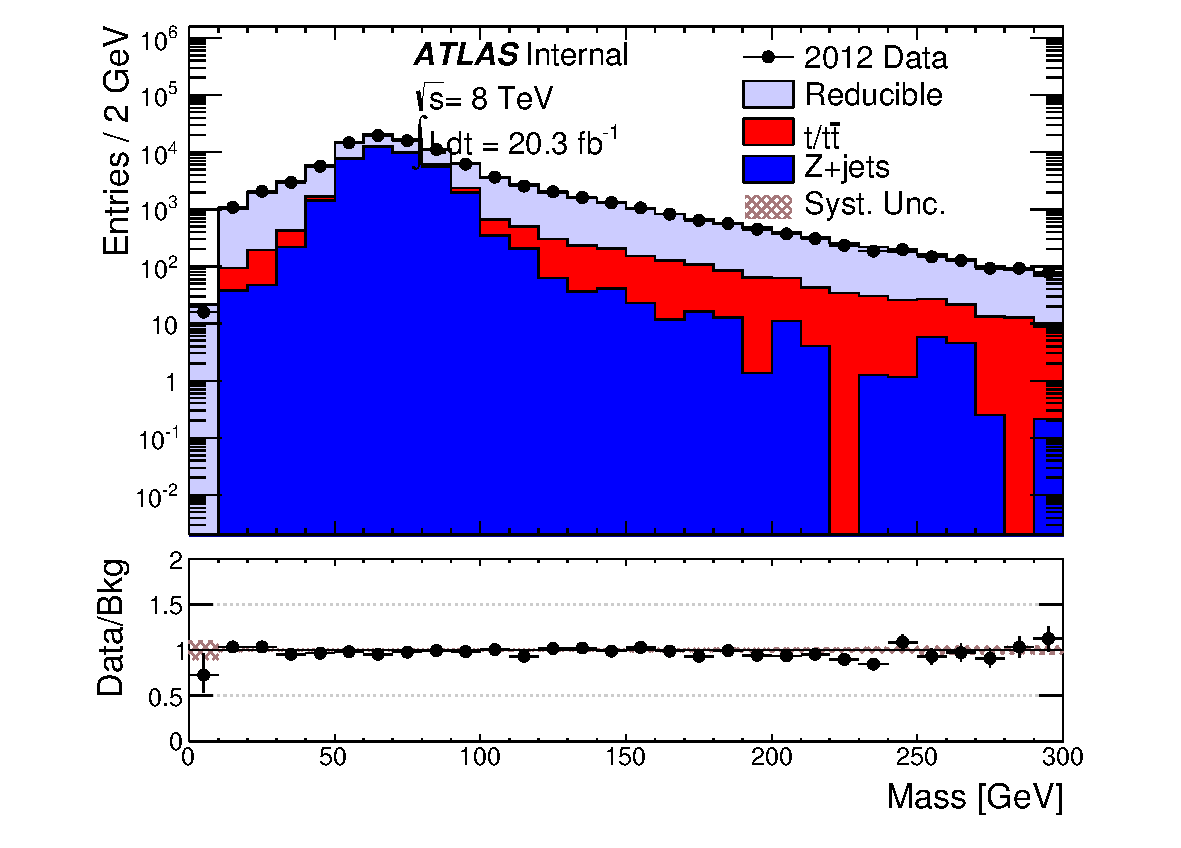
\includegraphics[width=0.48\textwidth]{figures/ch5-model-independent/TauFakes_ClosureMass}
%\centering 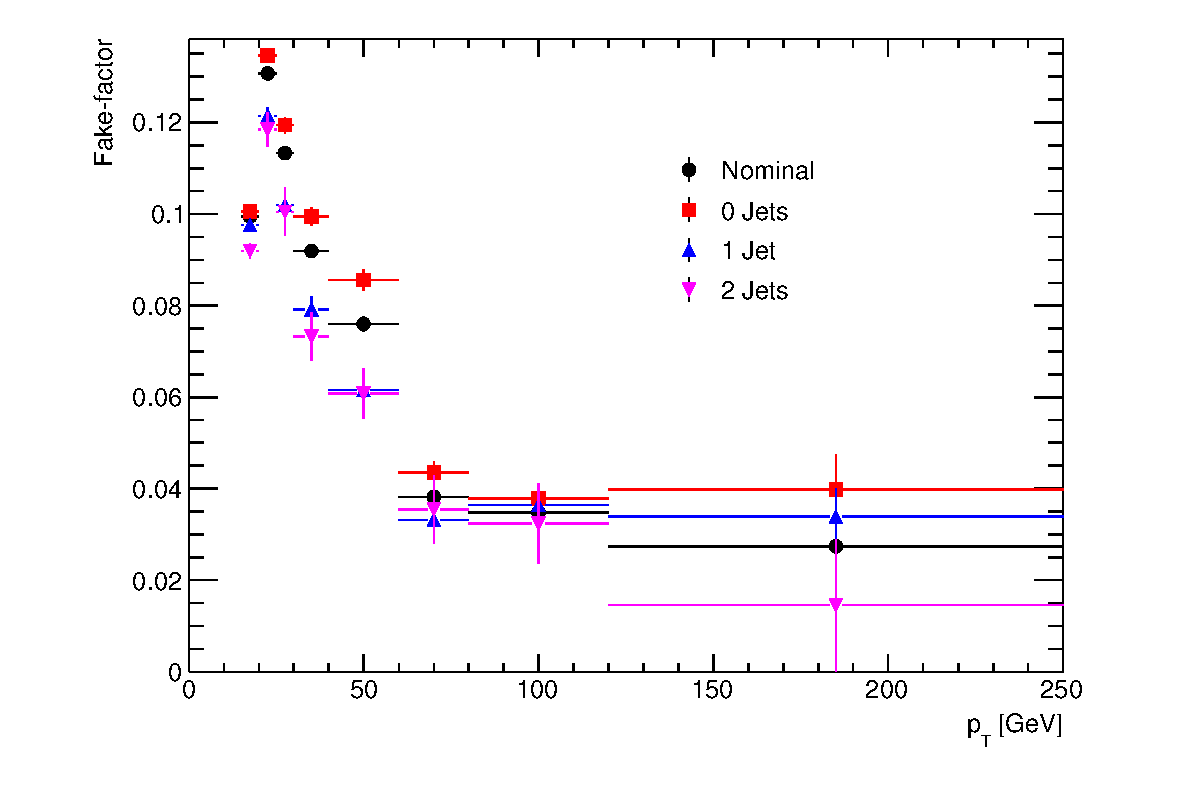
\includegraphics[width=0.48\textwidth]{figures/ch5-model-independent/TauFakes_NJetsDep}
\caption{\label{fig:tauclosure} Distributions of the $\tau$ p$_{T}$ (left), $\tau$ $\eta$
  (right), and invariant mass of the two leptons in the event (bottom).}
\end{figure}

%The uncertainty associated with the assumption that the fake-factors are entirely
%uncorrelated in ($p_{T}$, $\eta$) is evaluated by comparing the fake-factors obtained
%using a 2-D matrix in ($p_{T}$, $\eta$) and the product of the two 1-D fake-factors.  The
%RMS of the distribution is used to estimate the order of this effect, and is approximately
%15\%.

Finally, to estimate the sensitivity of the fake-factors to the flavour composition of the
sample used to derive them, the $t\bar{t}$ validation region described in~\ref{s:CR_Top}
is used. This sample was found in MC studies to have a largely different flavour
composition than the nominal $W$ + jets sample, and can therefore be used to put a
conservative systematic on this effect.  A flat variation of 25\% is found to bracket this
effect conservatively across all observables.

As a cross-check, the same effect can be probed less directly by tuning the requirements
of the $W$ + jets sample. The selection requirements applied to the $W$ + jets sample will
directly affect the kinematics and flavour composition of the sample, and lead to
differences in the derived fake-factors. While there is no direct way to measure how
different the compositions are between the $W$ + jets control sample and the signal
regions, it is possible to approximate how sensitive the fake-factors are to such changes.
Some selection requirements aimed at rejecting $Z$ + jets events are applied to derive
different sets of fake-factors, inspired by~\cite{zttnote,tauidnote}.  The following
requirements are applied separately:

\begin{itemize}
\item $\cos{\Delta\phi(\mu, \met)} + \cos{\Delta\phi(\tau, \met)} <$ -0.15
\item $m_{T}^{\mu} >$ 70 GeV
\item $m_{Z}^{vis.} <$ 42 GeV or $m_{Z}^{vis.} >$ 82 GeV
\item $p_{T}^{\mu} >$ 35 GeV
\end{itemize}

\begin{figure}
\centering 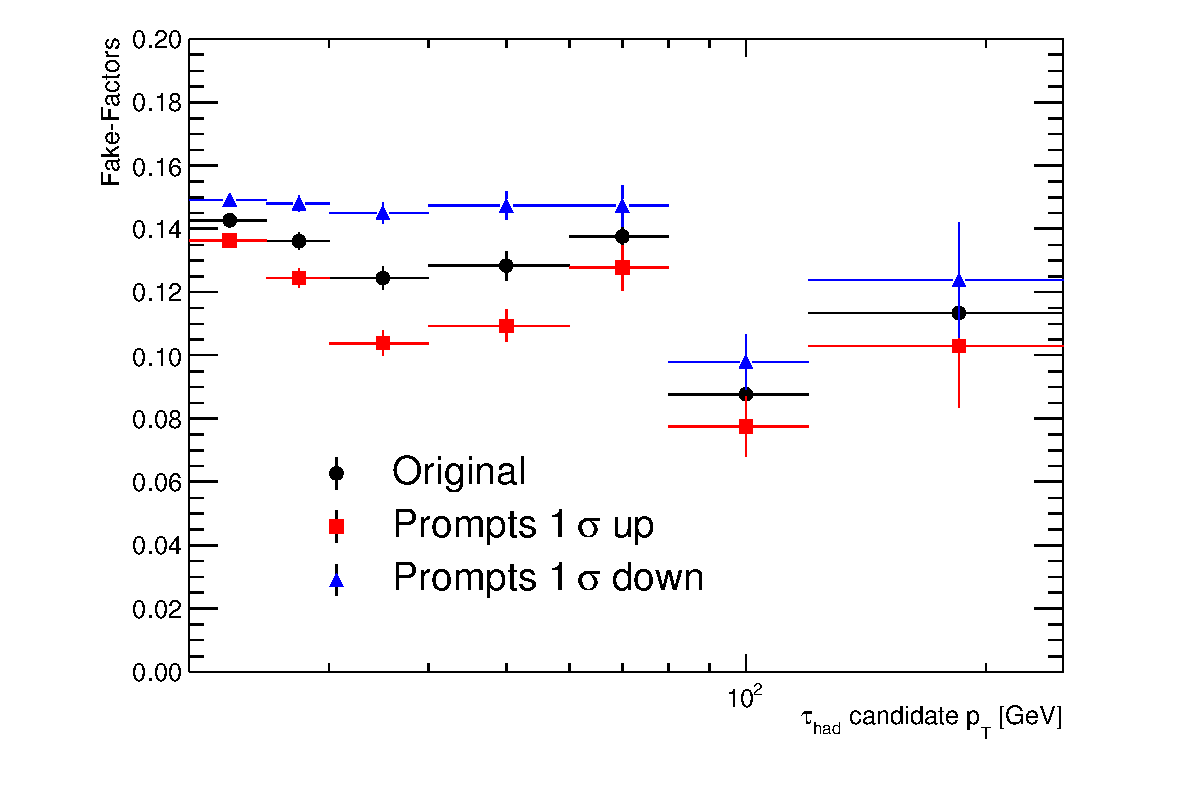
\includegraphics[width=0.48\textwidth]{figures/ch5-model-independent/TauFakes_PromptsDep}
\centering 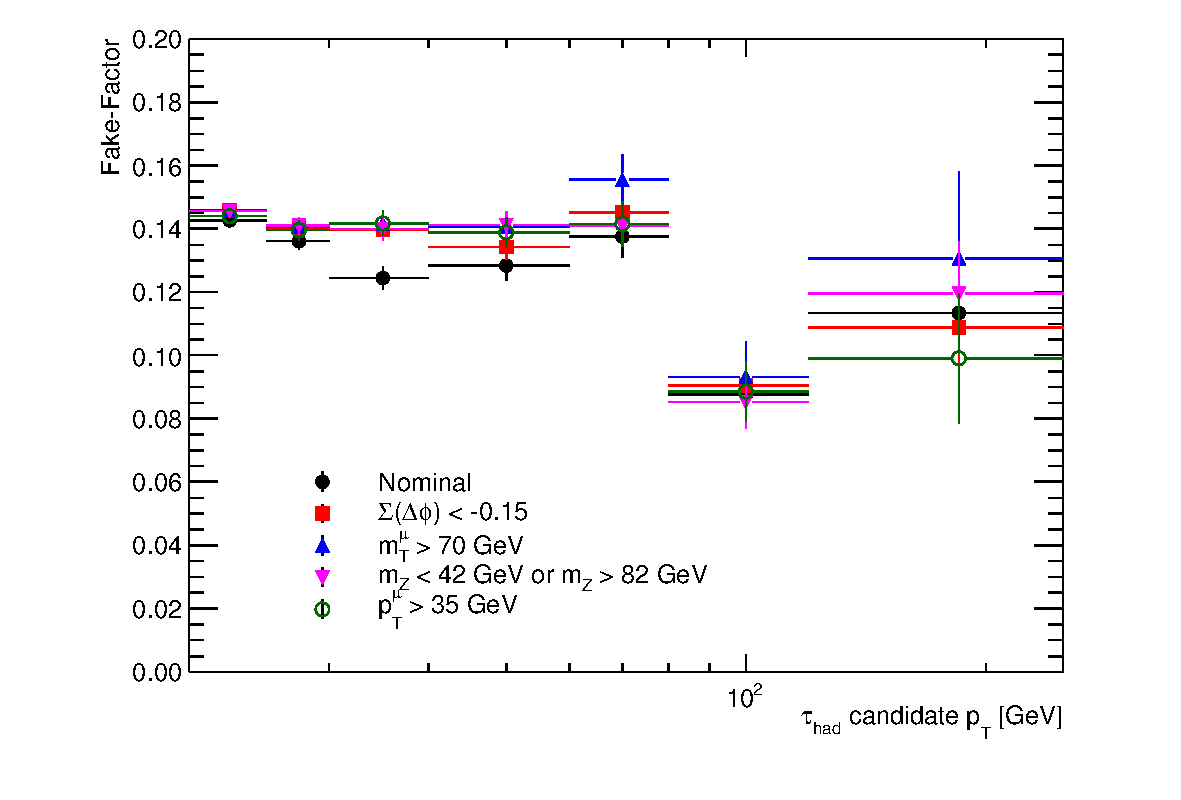
\includegraphics[width=0.48\textwidth]{figures/ch5-model-independent/TauFakes_CutsDep}
%\centering 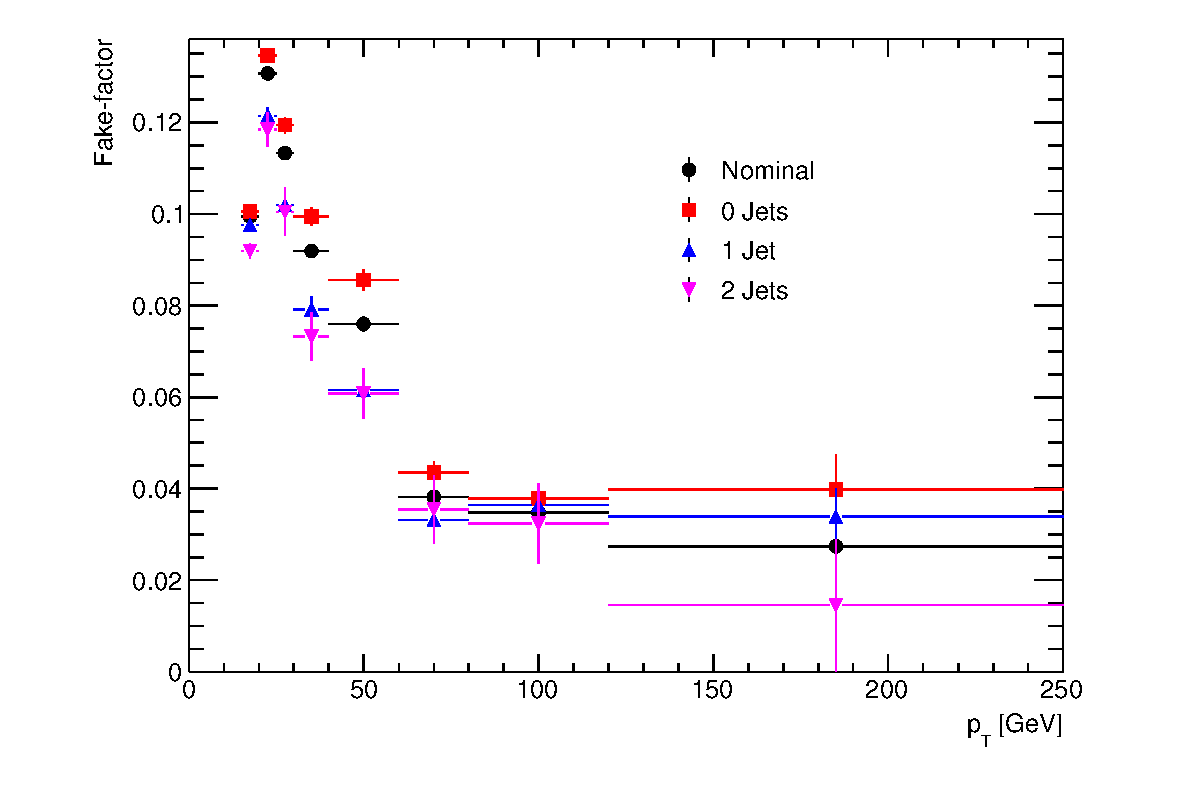
\includegraphics[width=0.48\textwidth]{figures/ch5-model-independent/TauFakes_NJetsDep}
\caption{\label{fig:fakesys} Dependency of the fake-factors on the prompt normalization
  (left) and the $W$ event requirements based on the cuts to reject $Z$ events (right).}
\end{figure}

The resulting sets of fake-factors are shown in figure~\ref{fig:fakesys}.  The variations
are no larger than 12\%, and are therefore bracketed by the 25\% estimate from the
$t\bar{t}$ sample.

In the end, the systematics are found to vary between 25\% and 30\%, being largest where
the prompt subtraction is most significant.


% Alternatively,
%making different requirements on the number of jets produced in association with the $W$
%leads to variations in the flavour composition of the sample. Fake-factors derived with
%different requirements on the number of jets are also shown in figure~\ref{fig:fakesys}.
%The scale of these variations due to different selection requirements on the $W$ + jets
%events is typically in the order of 20\% or less.


%Ultimately, a more direct way to probe how well the fake-factors model the reducible
%backgrounds consists in studying validation regions.  Three different validations regions are
%used, aimed at probing prompt and fake taus in $Z$-like and $t\bar{t}$ dilepton events,
%and in trilepton events where a $Z$ boson is well-reconstructed.  These 3 validation
%regions probe different topologies, and would reveal any mismodeling associated with this
%method.  Using the good degree of agreement found in the validation, and the magnitude of
%the effects studied above, a conservative flat uncertainty of 25\% is used for all $\tau$
%fake estimates.

\section{Systematic Uncertainties}\label{sec:model-independent-systematics}
Systematic uncertainties are assigned to the signal and background predictions to account for possible modelling inaccuracies. The sources of uncertainty considered are:

\begin{itemize}
	\item Uncertainties on the reducible background estimates from the data-driven estimation method, as described in section~\ref{sec:fake-factor-method}. The uncertainties ranges between $20\%$ to $30\%$ for the electron fake factors, $25\%$ to $50\%$ for the muon fake factors, and $25\%$ to $30\%$ for the tau lepton fake factors.

	\item The signal and background samples must be normalized to the integrated luminosity of the data. The weight assigned to each event is:
	\begin{equation}
		w = \frac{\mathcal{L} \sigma_{\mathrm{process}}}{N_{\mathrm{sim}}},
	\end{equation}
	where $\mathcal{L}$ is the integrated luminosity of the data, $\sigma_{\mathrm{process}}$ is the cross section of the simulated process, and $N_{\mathrm{sim}}$ is the number of simulated events. The integrated luminosity carries an uncertainty of $2.8\%$, as described in section~\ref{sec:luminosity-measurement}. The cross sections are taken from calculations with uncertainties due to various sources, including the fixed order of the calculation, the choice of renormalization and factorization scales, and the PDFs. The uncertainties are shown in table~\ref{table:model-independent-cross-section-uncertainties}. 

\begin{table}
  \begin{center}
    \begin{tabular}{c r c}
      \hline
      Sample     &Uncertainty &Reference\\
      \hline
      $Z$+jets   &10\% \\
      $\ttbar+V$ &22\% &\cite{ttV} \\
      $ZZ$       &4.3\% &App.~\ref{app:vbfnlo} \\
      $WZ$       &7.6\% &App.~\ref{app:vbfnlo}\\
      $\ttbar$   &10\% &\cite{TopXS} \\
      single-$t$ &10\% &\cite{atlas_topmc}\\
      \hline
    \end{tabular}
    \caption{Systematic uncertainties used for the MC samples that contribute to the background estimates.}
    \label{tab:modle-independent-cross-section-uncertainties}
  \end{center}
\end{table}


	\item Events are also weighted to account for differences between data and Monte Carlo simulation in the lepton trigger, reconstruction, and identification efficiencies. The scale factors and associated uncertainties are provided by the relevant ATLAS combined performance groups. The electron and muon scale factors are close to unity, with uncertainties in the range $1$-$5\%$. The scale factors for the tau lepton identification efficiency range from $94$-$96\%$ for the \texttt{BDTTight} working point, and carry uncertainties between $2.0$-$2.2\%$~\cite{TauUncertainties}.

	\item The lepton energy scales carry uncertainty which has a small effect on the signal regions due to leptons or events near $\Et$ or $\pt$ thresholds. The uncertainties are also provided by the combined performance groups.

	\item  The jet energies are scaled and smeared according to recommendations from the \texttt{JetEtMiss} combined performance group~\cite{JES,JER}. The uncertainty affects the $\Htjets$ and $\meff$ distributions, and also the lepton-jet overlap removal procedure.

	\item The lepton and jet energy uncertainties are also propagated to the missing transverse energy, $\Etmiss$, using the \texttt{MissingETUtility} package~\cite{METUtility}. 

	\item The efficiencies of the $b$-tagging algorithm carry uncertainties which are parameterized based on matching the identified $b$-jets to truth $b$-jets, as recommended by the \texttt{flavor tagging} combined performance group.

	\item Finally, the Monte Carlo samples carry statistical uncertainty due to simulating a finite number of events. 
\end{itemize}

The dominant sources of uncertainty depend on the signal region, but are generally due to Monte Carlo statistical uncertainties, the fake factor uncertainites, and theoretical cross section uncertainties. 

\section{Background Validation}\label{sec:model-independent-validation-regions}
The background estimates are verified in several dedicated validation regions, which are orthogonal to the signal regions. Events containing two leptons are used to test the selection of prompt leptons and their corresponding scale factors and energy corrections. The reducible backgrounds are tested in $t\overline{t}$ validation regions, where the events are required to have two same-sign leptons to target semileptonic decays where one lepton arises from a reducible process. Finally, the fake factor procedure is validation in events with modified lepton selections, where the signal leptons are ``between'' the numerator and denominator definitions used in the nominal reducible background estimate.

\subsection{Dilepton Validation Regions}\label{sec:model-independent-validation-regions-dilepton}
Three dilepton validation regions target the three flavors of leptons: $ee$, $\mu\mu$, and $\mu\tau_{\mathrm{had}}$. The $ee$ and $\mu\mu$ regions require an opposite-sign lepton pair of the appropriate flavor. The invariant mass distributions of the dilepton system in these regions are shown in figure~\ref{fig:model-independent-VR-dilepton}. Some disagreement is observed in the $ee$ invariant mass distribution; this discrepancy is covered by the electron energy scale systematic uncertainties. 

\begin{figure}[htbp]
  \subfloat[$ee$]{
    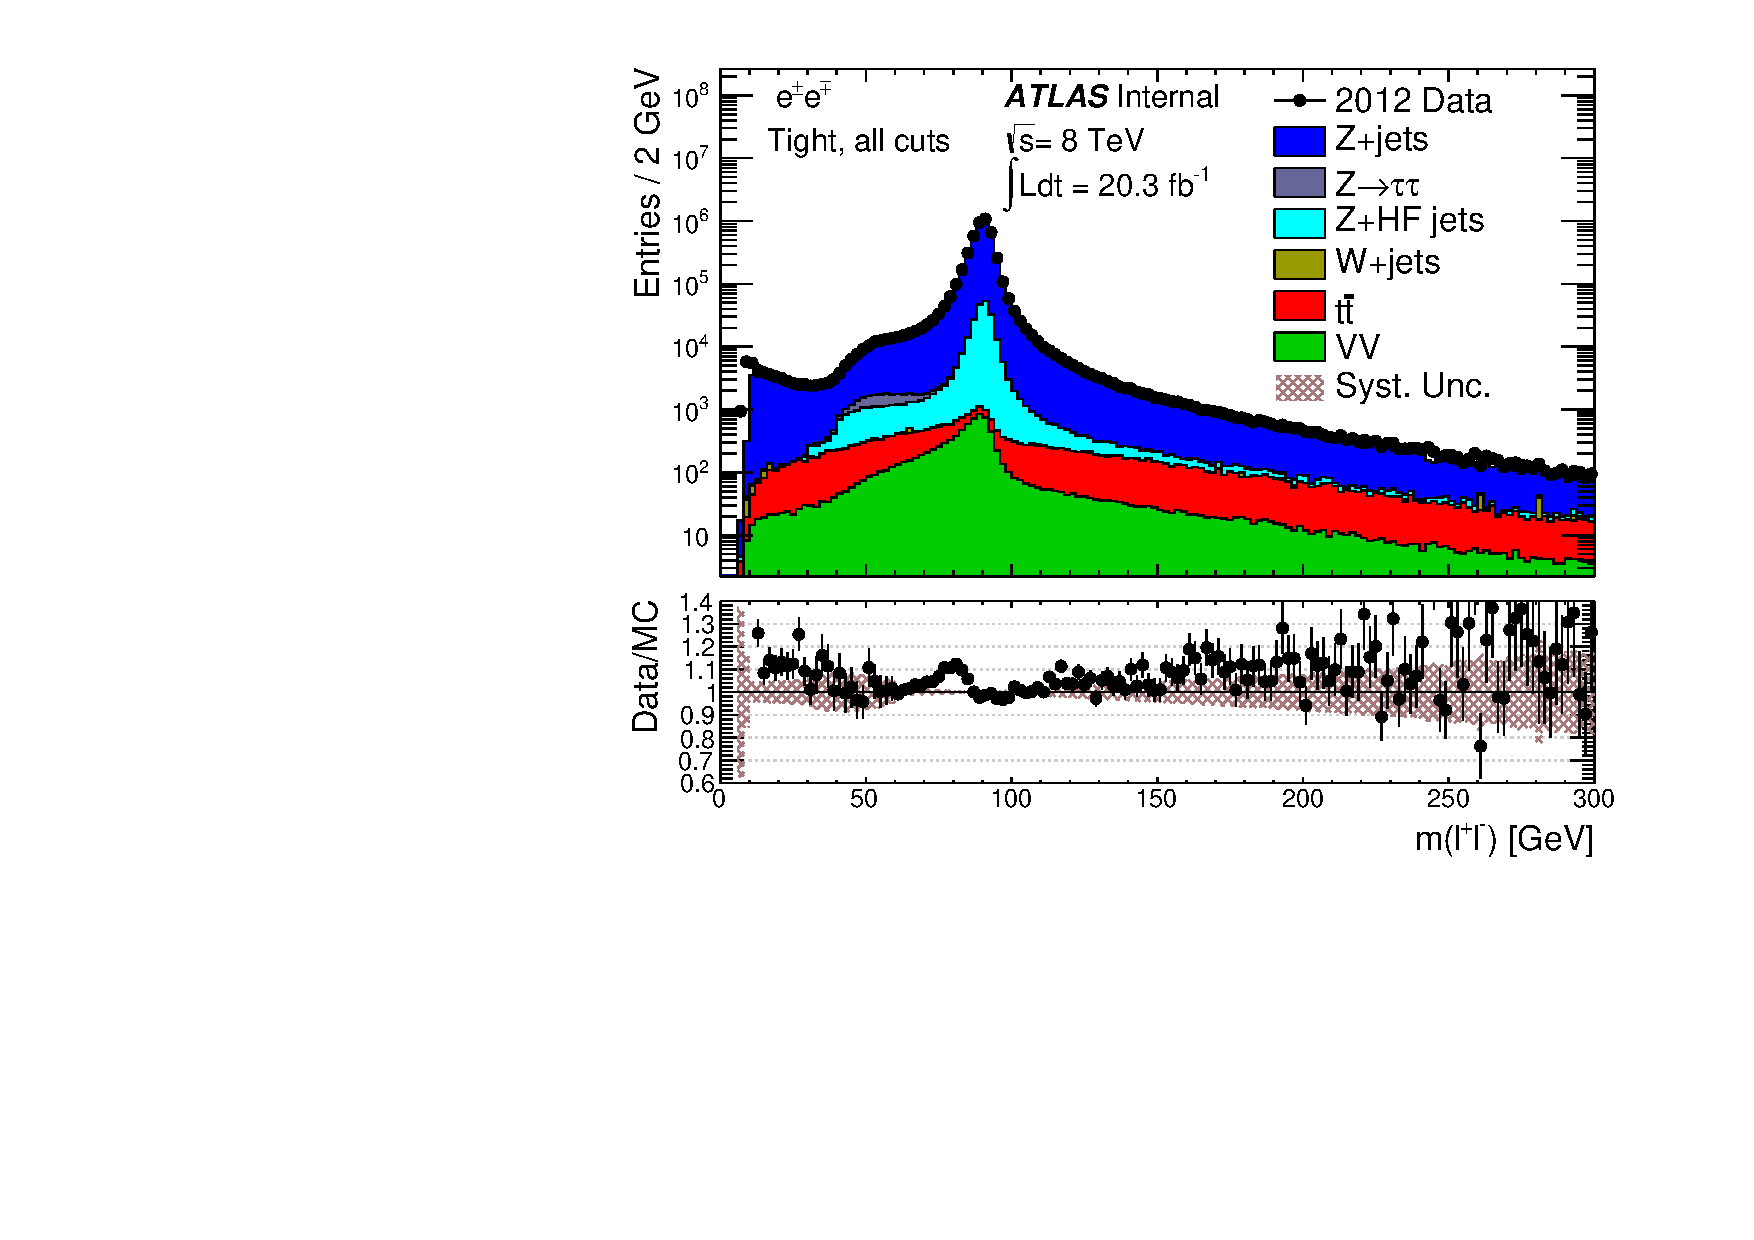
\includegraphics[width=.48\columnwidth]{figures/ch5-model-independent/DYOSee_cut_3f_AllLeptonMass}
  }
  \subfloat[$\mu\mu$]{
    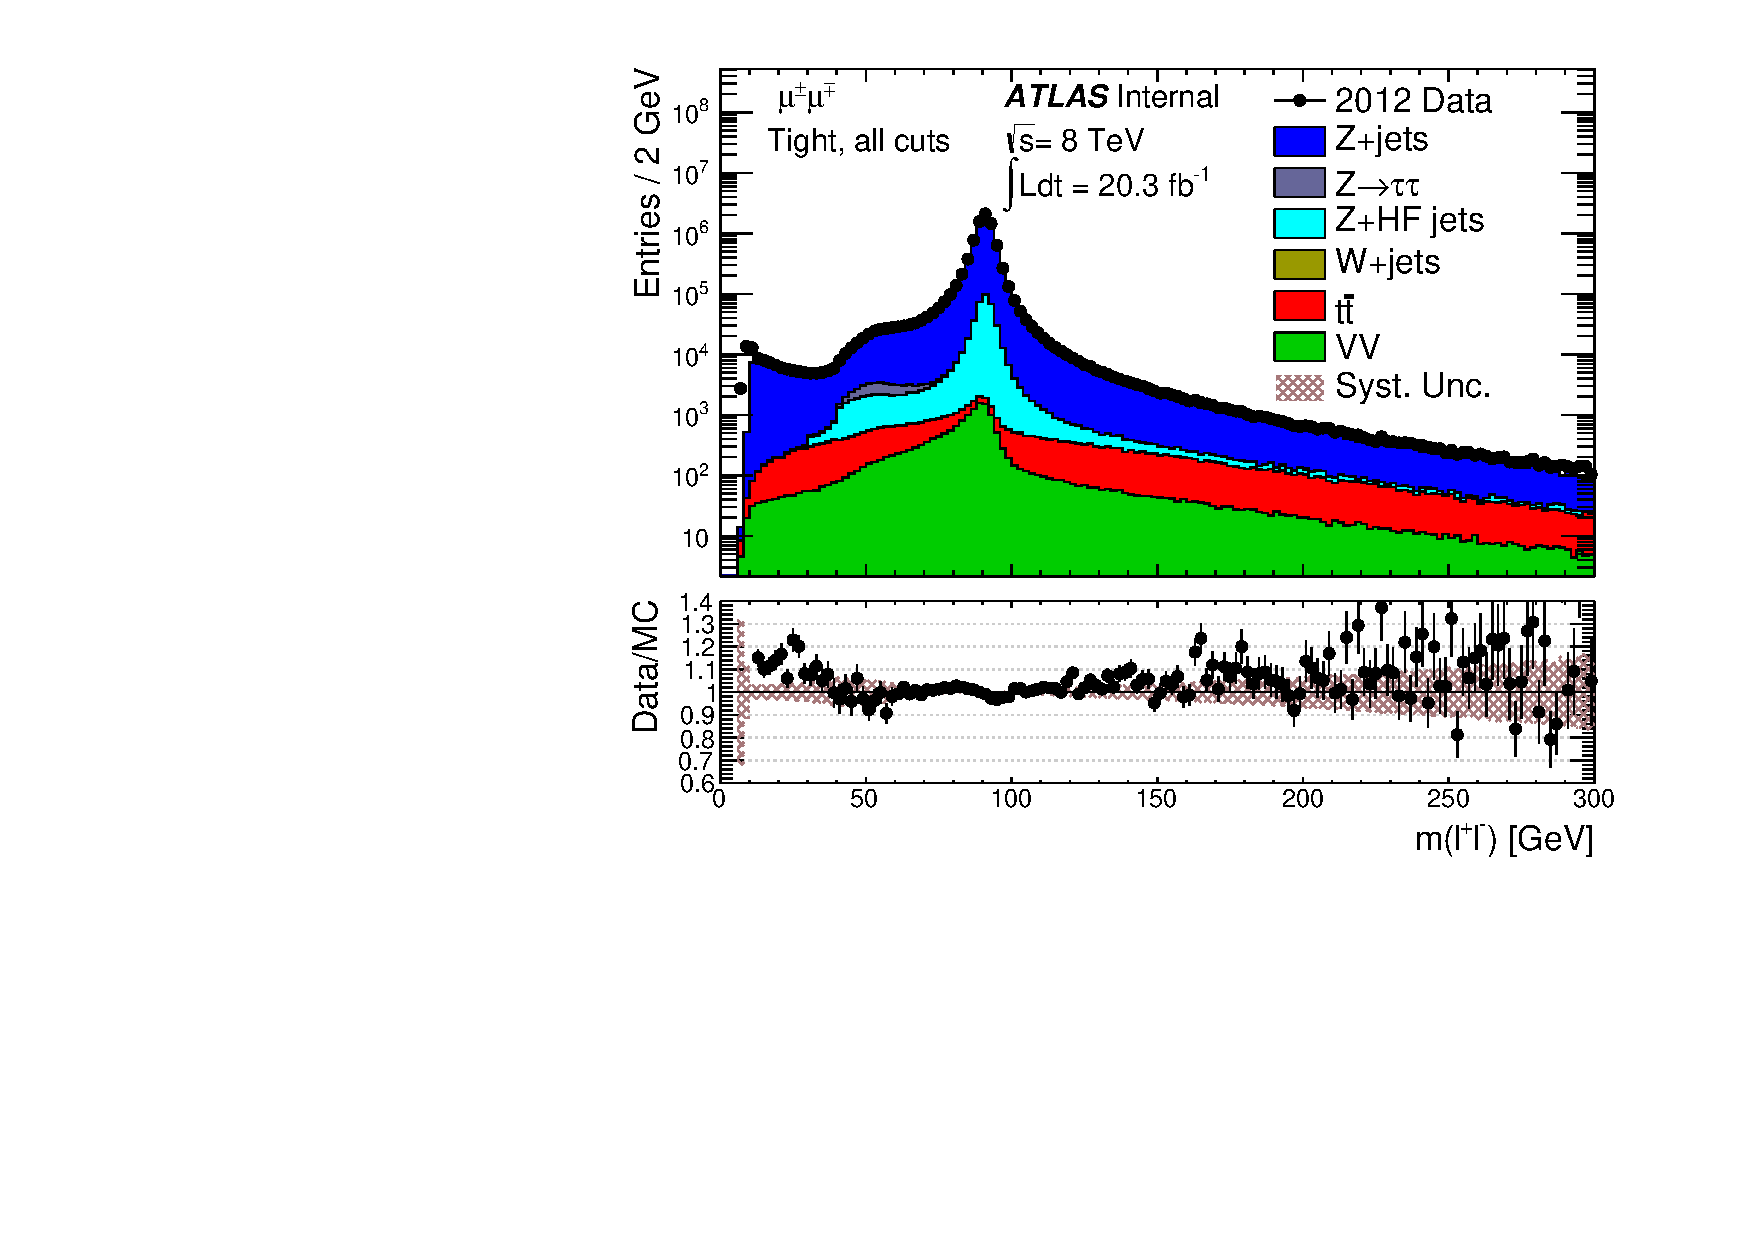
\includegraphics[width=.48\columnwidth]{figures/ch5-model-independent/DYOSmm_cut_3f_AllLeptonMass}
  }
  \caption{Dilepton invariant mass distributions for the $ee$ (left) and $\mu\mu$ (right) validation regions.}
  \label{fig:dilepton_masses}
\end{figure}

The $ee$ and $\mu\mu$ validation regions are also used to generate scale factors to account for efficiency
differences between simulation and data when applying cuts on lepton isolation or impact parameter. The scale factors are computed from events with a dilepton pair with invariant mass within $10 \GeV$ of $m_Z$, and are shown in figure~\ref{fig:model-independent-lepton-SFs}. The scale factors are mostly consistent with unity to within $0.5\%$, except for isolation requirements on the low-$\pt$ leptons, where the scale factors deviate from unity by up to $2\%$. 

\begin{figure}[tbp]
  \subfloat[Electron \pt\ Scale Factors]{
    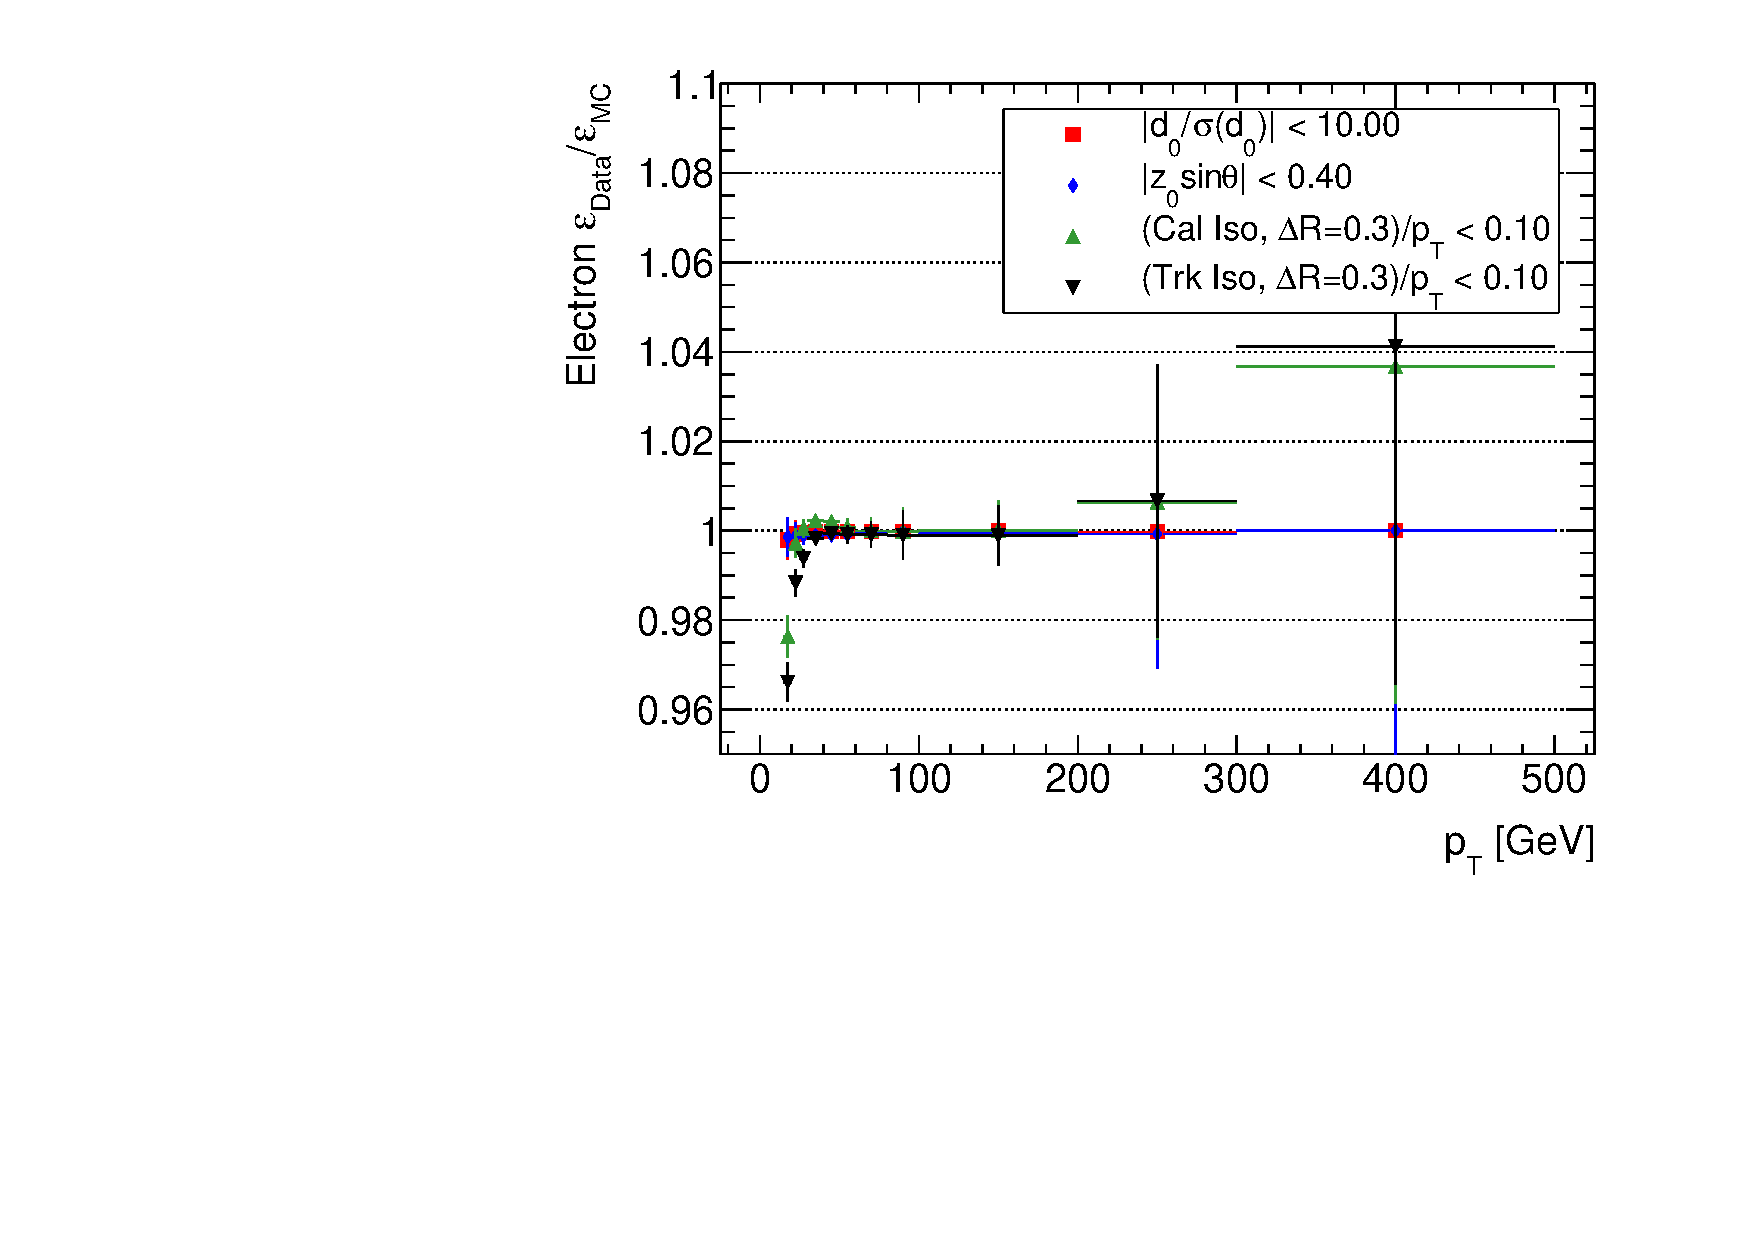
\includegraphics[width=.48\columnwidth]{figures/ch5-model-independent/c_e_pt_allSF}
  }
  \subfloat[Electron $|\eta|$ Scale Factors]{
    \includegraphics[width=.48\columnwidth]{figures/ch5-model-independent/c_e_eta_allSF}
  }
  \subfloat[Muon \pt\ Scale Factors]{
    \includegraphics[width=.48\columnwidth]{figures/ch5-model-independent/c_m_pt_allSF}
  }
  \subfloat[Muon $|\eta|$ Scale Factors]{
    \includegraphics[width=.48\columnwidth]{figures/ch5-model-independent/c_m_eta_allSF}
  }
  \caption{Scale factors for electrons and muons as functions of \pt\ (left) and $|\eta|$ (right).}
  \label{fig:lepton_SFs}
\end{figure}

The $\mu\tau_{\mathrm{had}}$ region applies addition cuts to reduce the large contribution from fake tau leptons in $W$+jets events:

\begin{itemize}
	\item $\cos{\Delta\phi(\mu, \met)} + \cos{\Delta\phi(\tau, \met)} >$ -0.15,
	\item $\Delta\phi(\mu, \tau_{had}) >$ 2.4,
	\item $m_{\mathrm{T}}^{\mu} < 50 \GeV$,
	\item $42< m_{Z}^{vis.} < 82 \GeV$, and
	\item $\pt^{\mu} < 40 \GeV$.
\end{itemize}

The $\pt$ and $\eta$ distributions of the $\mu$ and $\tau_{\mathrm{had}}$ are shown in figure~\ref{fig:model-independent-VR-mutau}.

\begin{figure}[htbp]
	\subfloat[Leading Lepton \pt]
		{\includegraphics[width=.48\columnwidth]{figures/ch5-model-independent/OSZ_LeadingPt}}
	\subfloat[Leading Lepton $|\eta|$]
		{\includegraphics[width=.48\columnwidth]{figures/ch5-model-independent/OSZ_LeadingEta}}
	\subfloat[Subleading Lepton \pt]
		{\includegraphics[width=.48\columnwidth]{figures/ch5-model-independent/OSZ_SubleadPt}}
	\subfloat[Subleading Lepton $|\eta|$]
		{\includegraphics[width=.48\columnwidth]{figures/ch5-model-independent/OSZ_SubleadEta}}
	\caption{$\pt$ and $\eta$ distribution of the muon and the hadronically decaying tau lepton in the $\mu\tau_{\mathrm{had}}$ validation region.}
	\label{fig:model-independent-VR-mutau}
\end{figure}


\subsection{$t\overline{t}$ Validation Regions}\label{sec:model-independent-validation-regions-ttbar}
In signal regions that veto $Z$ bosons and require large $\Htjets$ or $\Etmiss$, a large reducible background component is expected from $t\overline{t}$ events, where both $W$ bosons decay leptonically and a third lepton arises from a misidentified jet or semileptonic heavy flavor decay. This process is tested in the $t\overline{t}$ validation regions, which require at least one $b$-tagged jet with $\pt>30 \GeV$, exactly two electrons or muons with the same charge, and $\Ht<500 \GeV$. The requirement that the leptons have the same sign vetoes dilepton $t\overline{t}$ events with two prompt leptons from $W$ decays, while the $\Ht$ requirement reduces the potential contamination from new BSM phenomena. Note that events containing hadronically decaying tau leptons are used to derive a systematic uncertainty on the tau fake factors due to the flavor composition of the events (section~\ref{sec:model-independent-ff-tau-systematics}), and so are not used as a validation region. 

The $\pt$ and $\eta$ distributions of the leading and subleading leptons are shown in figure~\ref{fig:model-independent-VR-ttbar}.

\begin{figure}[tbp]
  \subfloat[Leading Lepton \pt]{\includegraphics[width=.48\columnwidth]{figures/ch5-model-independent/semileptop_emu_mue_LeadPt}}
  \subfloat[Leading Lepton $|\eta|$]{\includegraphics[width=.48\columnwidth]{figures/ch5-model-independent/semileptop_emu_mue_LeadEta}}
  \subfloat[Subleading Lepton \pt]{\includegraphics[width=.48\columnwidth]{figures/ch5-model-independent/semileptop_emu_mue_SubleadPt}}
  \subfloat[Subleading Lepton $|\eta|$]{\includegraphics[width=.48\columnwidth]{figures/ch5-model-independent/semileptop_emu_mue_SubleadEta}}
  \subfloat[\meff]{\includegraphics[width=.48\columnwidth]{figures/ch5-model-independent/semileptop_emu_mue_ST}}
  \subfloat[\met]{\includegraphics[width=.48\columnwidth]{figures/ch5-model-independent/semileptop_emu_mue_MET}}
  \caption{\ttbar\ validation regions for all flavor ($e, \mu$) combinations.}
  \label{fig:model-independent-VR-ttbar}
\end{figure}

\subsection{Intermediate Fake Factor Validation Regions}\label{sec:model-independent-validation-regions-intermediate-ff}
The fake factor method is further validated in regions containing events with two signal (numerator) leptons and one ``intermediate'' lepton, which fulfills selection criteria looser than the numerator criteria but tighter than the denominator criteria. Separate fake factors are derived for intermediate leptons; these are defined schematically as $\langle$intermediate$\rangle/\langle$denominator$\rangle$, rather than $\langle$numerator$\rangle/\langle$denominator$\rangle$. Specifically, the intermediate leptons satisfy most of the numerator criteria except for:

\begin{itemize}
	\item \textbf{Electrons}: the electron must pass the \texttt{medium++} cuts, but fail the \texttt{tight++} cuts.  
	\item \textbf{Muons}: the candidate must have either its track or calorimeter transverse isolation energy
	satisfy $0.10 < \mathrm{iso}/\pt < 0.15$.
	\item \textbf{Taus}: the tau candidate must pass the \texttt{Medium-BDT} identification requirement, but fail the
	\texttt{tight-BDT} identification requirement.
\end{itemize}

The first two regions, targeting reducible electrons and muons, require an OSSF pair of electrons or muons, plus a third intermediate electron or muon of different flavor. The events are largely due to $Z\rightarrow ee$ or $Z\rightarrow \mu\mu$ events, with an additional lepton that is either prompt and fails the signal lepton criteria, or is due to a reducible process. 

\begin{figure}[tbp]\centering
  \subfloat[Event Composition]{\includegraphics[width=.48\columnwidth]{figures/ch5-model-independent/Z_emu_Zmm_offZe_intelec_Simple3LEventClassification}}
  \subfloat[Electron \pt]{\includegraphics[width=.48\columnwidth]{figures/ch5-model-independent/Z_emu_Zmm_offZe_intelec_OffZPt}}
  \subfloat[Electron $\eta$]{\includegraphics[width=.48\columnwidth]{figures/ch5-model-independent/Z_emu_Zmm_offZe_intelec_OffZEta}}
  \subfloat[Electron \mt]{\includegraphics[width=.48\columnwidth]{figures/ch5-model-independent/Z_emu_Zmm_offZe_intelec_OffZMT}}
  \subfloat[\meff]{\includegraphics[width=.48\columnwidth]{figures/ch5-model-independent/Z_emu_Zmm_offZe_intelec_ST}}
  \subfloat[\met]{\includegraphics[width=.48\columnwidth]{figures/ch5-model-independent/Z_emu_Zmm_offZe_intelec_MET}}
  \caption{Expected backgrounds in the intermediate-electron validation region, using the
    nominal background estimation techniques.}
  \label{fig:model-independent-VR-intermediate-e}
\end{figure}

\begin{figure}[tbp]\centering
  \subfloat[Event Composition]{\includegraphics[width=.48\columnwidth]{figures/ch5-model-independent/Z_emu_Zee_offZmu_intmuon_Simple3LEventClassification}}
  \subfloat[Muon \pt]{\includegraphics[width=.48\columnwidth]{figures/ch5-model-independent/Z_emu_Zee_offZmu_intmuon_OffZPt}}
  \subfloat[Muon $\eta$]{\includegraphics[width=.48\columnwidth]{figures/ch5-model-independent/Z_emu_Zee_offZmu_intmuon_OffZEta}}
  \subfloat[Muon
    \mt]{\includegraphics[width=.48\columnwidth]{figures/ch5-model-independent/Z_emu_Zee_offZmu_intmuon_OffZMT}}
  \subfloat[\meff]{\includegraphics[width=.48\columnwidth]{figures/ch5-model-independent/Z_emu_Zee_offZmu_intmuon_ST}}
  \subfloat[\met]{\includegraphics[width=.48\columnwidth]{figures/ch5-model-independent/Z_emu_Zee_offZmu_intmuon_MET}}
  \caption{Expected backgrounds in the intermediate-muon validation region, using the
    nominal background estimation techniques.}
  \label{fig:model-independent-VR-intermediate-mu}
\end{figure}

The events containing an intermediate $\tau_{\mathrm{had}}$ are much more abundant than intermediate electrons or muons, so three $\tau_{\mathrm{had}}$ validation regions are defined, mirroring the signal region categories. Events are required to contain two electrons or muons plus an intermediate $\tau_{\mathrm{had}}$, and are separated into on-$Z$, off-$Z$/OSSF, and off-$Z$/mixed categories, depending on the two electrons or muons. The $\pt$ and $\eta$ of the intermediate $\tau_{\mathrm{had}}$ is shown for each category in figure~\ref{fig:model-independent-VR-intermediate-tau}.

\begin{figure}[tbp]\centering
  \subfloat[Intermediate $\tau_{\mathrm{had}}$ $p_{T}$, on-$Z$]{\includegraphics[width=.44\columnwidth]{figures/ch5-model-independent/inttau_onZ_DY_TauPt}}
  \subfloat[Intermediate $\tau_{\mathrm{had}}$ $\eta$, on-$Z$]{\includegraphics[width=.44\columnwidth]{figures/ch5-model-independent/inttau_onZ_DY_TauEta}}
  \subfloat[Intermediate $\tau_{\mathrm{had}}$ $p_{T}$, off-$Z$/OSSF]{\includegraphics[width=.44\columnwidth]{figures/ch5-model-independent/inttau_offZ_OSSF_DY_TauPt}}
  \subfloat[Intermediate $\tau_{\mathrm{had}}$ $\eta$, off-$Z$/OSSF]{\includegraphics[width=.44\columnwidth]{figures/ch5-model-independent/inttau_offZ_OSSF_DY_TauEta}}
  \subfloat[Intermediate $\tau_{\mathrm{had}}$ $p_{T}$, off-$Z$/mixed]{\includegraphics[width=.44\columnwidth]{figures/ch5-model-independent/inttau_offZ_mixed_DY_TauPt}}
  \subfloat[Intermediate $\tau_{\mathrm{had}}$ $\eta$, off-$Z$/mixed]{\includegraphics[width=.44\columnwidth]{figures/ch5-model-independent/inttau_offZ_mixed_DY_TauEta}}
  \subfloat[Intermediate tau $m_{T}$]

  \caption{$\pt$ and $\eta$ distributions of the intermediate $\tau_{\mathrm{had}}$ in the on-$Z$, off-$Z$/OSSF, and off-$Z$/mixed intermediate validation regions. }
  \label{fig:model-independent-VR-intermediate-tau}
\end{figure}


\section{Results and Limits}\label{sec:model-independent-results}
The results of the search as organized as follows. For each category, the distributions of the various kinematic variables ($\htlep$, $\htjets$, $\meff$, $\Etmiss$, $\mtw$, $N_{\mathrm{jets}}$, $N_{b-\mathrm{tags}}$, and the $\pt$ of the third lepton) are produced (where applicable). Then, in each of the 138 signal regions, the number of observed and expected events are compared, and, absent any significant deviations, $95\%$ confidence level (CL) upper limits are derived on the number of events from new physics, $N_{95}$, and the corresponding \emph{visible cross section}, $\sigma_{95}^{\mathrm{vis}}$, defined as

\begin{equation}
	\sigma_{95}^{\mathrm{vis}} = \frac{N_{95}}{\mathcal{L}},
\end{equation}

where $\mathcal{L}=20.3~\mbox{fb}^{-1}$ is the integrated luminosity of the data.

The plots for the $\htlep$ signal regions are shown here for demonstrative purposes. The full set of plots is available at~\cite{model-independent-webpage}. The $\htlep$ distributions are shown in figure~\ref{fig:model-independent-htlep}. The observed and expected event counts in the three corresponding signal regions ($\htlep>200 \GeV$, $\htlep>500 \GeV$, and $\htlep>800 \GeV$) are shown in table~\ref{table:model-independent-htlep}. Finally, the upper limits on $\sigma_{95}^{\mathrm{vis}}$ are shown in figure~\ref{fig:model-independent-htlep-sigmavis}. 

The deviations between the observed and expected in all 138 signal regions are shown in figure~\ref{fig:model-independent-summary-sigma}, in units of the total uncertainty on the background expectation. 

\begin{figure}[htbp]
	\centering

	\caption{$\htlep$ distributions in the six categories.}
	\label{fig:model-independent-htlep}
\end{figure}

\begin{table}[htbp]
	\centering

	\caption{Observed and expected event counts in the $\htlep$ signal regions, along with the inclusive counts for the entire category.}
	\label{table:model-independent-htlep}
\end{table}

\begin{figure}
	\centering

	\caption{95\% CL upper limits on the visible cross section of trilepton event production from new physics, $\sigma_{95}^{\mathrm{vis}}$, in each $\htlep$ signal region. }
	\label{fig:model-independent-htlep-sigmavis}
\end{figure}

\begin{figure}
	\centering

	\caption{Deviations between the observed event counts and the background expectations in each signal region, in units of the total uncertainty on the background prediction.}
	\label{fig:model-independent-summary-sigma}
\end{figure}



\section{Interpretations}
The 95\% CL upper limits on trilepton event production from new physics derived in section~\ref{sec:model-independent-results} provide a useful tool with which to confront models of new physics producing trilepton final states. In order to compare the predictions of a model, i.e. a set of simulated events at \textcolor{red}{particle level} from an event generator, per-lepton fiducial efficiencies are provided to quantify approximately the efficiency of reconstructing and selecting fiducial leptons at truth level. The definition of fiducial truth leptons is as follows: 

\begin{itemize}
	\item \underline{\textbf{Transverse momentum}}: Electrons and muons are required to have $\pt>10 \GeV$, while tau leptons are required to have $\pt>15 \GeV$.
	\item \underline{\textbf{Pseudorapidity}}: The same pseudorapidity cuts as the reconstructed signal leptons are applied. Electrons must have $|\eta|<2.47$, excluding the region $1.37<|\eta|<1.52$, and muons and tau leptons must have $|\eta|<2.5$.
	\item \underline{\textbf{Isolation}}: For electrons and muons, the sum of the transverse momenta of all charged particles with $\pt>1 \GeV$ within a cone of radius $\Delta R=0.3$ of the lepton, denoted \texttt{truth\_ptcone30}, must satisfy \texttt{truth\_ptcone30}/$\pt<0.15$. Similarly, the \texttt{truth\_Etcone30}, defined as the sum of all stable, visible particles within a cone of radius $\Delta R=0.3$, is required to satisfy \texttt{truth\_Etcone30}$/\pt<0.15$.
	\item \underline{\textbf{Origin and Decay}}: Leptons must originate from the hard scattering interaction (as opposed to the interaction with the detector as simulated by \geant), and not arise from the decay of a hadron. Electrons and muons are also required to be stable; tau leptons are required to decay hadronically. 
\end{itemize}

The efficiencies are derived from a Monte Carlo simulation sample 

\textcolor{red}{Efficiencies. Doubly charged higgs interpretation?}